% Options for packages loaded elsewhere
\PassOptionsToPackage{unicode}{hyperref}
\PassOptionsToPackage{hyphens}{url}
%
\documentclass[
]{book}
\usepackage{amsmath,amssymb}
\usepackage{lmodern}
\usepackage{ifxetex,ifluatex}
\ifnum 0\ifxetex 1\fi\ifluatex 1\fi=0 % if pdftex
  \usepackage[T1]{fontenc}
  \usepackage[utf8]{inputenc}
  \usepackage{textcomp} % provide euro and other symbols
\else % if luatex or xetex
  \usepackage{unicode-math}
  \defaultfontfeatures{Scale=MatchLowercase}
  \defaultfontfeatures[\rmfamily]{Ligatures=TeX,Scale=1}
\fi
% Use upquote if available, for straight quotes in verbatim environments
\IfFileExists{upquote.sty}{\usepackage{upquote}}{}
\IfFileExists{microtype.sty}{% use microtype if available
  \usepackage[]{microtype}
  \UseMicrotypeSet[protrusion]{basicmath} % disable protrusion for tt fonts
}{}
\makeatletter
\@ifundefined{KOMAClassName}{% if non-KOMA class
  \IfFileExists{parskip.sty}{%
    \usepackage{parskip}
  }{% else
    \setlength{\parindent}{0pt}
    \setlength{\parskip}{6pt plus 2pt minus 1pt}}
}{% if KOMA class
  \KOMAoptions{parskip=half}}
\makeatother
\usepackage{xcolor}
\IfFileExists{xurl.sty}{\usepackage{xurl}}{} % add URL line breaks if available
\IfFileExists{bookmark.sty}{\usepackage{bookmark}}{\usepackage{hyperref}}
\hypersetup{
  pdftitle={Analyse og visualisering af biologiske datasæt - 2022},
  pdfauthor={Sarah Rennie},
  hidelinks,
  pdfcreator={LaTeX via pandoc}}
\urlstyle{same} % disable monospaced font for URLs
\usepackage{color}
\usepackage{fancyvrb}
\newcommand{\VerbBar}{|}
\newcommand{\VERB}{\Verb[commandchars=\\\{\}]}
\DefineVerbatimEnvironment{Highlighting}{Verbatim}{commandchars=\\\{\}}
% Add ',fontsize=\small' for more characters per line
\usepackage{framed}
\definecolor{shadecolor}{RGB}{248,248,248}
\newenvironment{Shaded}{\begin{snugshade}}{\end{snugshade}}
\newcommand{\AlertTok}[1]{\textcolor[rgb]{0.94,0.16,0.16}{#1}}
\newcommand{\AnnotationTok}[1]{\textcolor[rgb]{0.56,0.35,0.01}{\textbf{\textit{#1}}}}
\newcommand{\AttributeTok}[1]{\textcolor[rgb]{0.77,0.63,0.00}{#1}}
\newcommand{\BaseNTok}[1]{\textcolor[rgb]{0.00,0.00,0.81}{#1}}
\newcommand{\BuiltInTok}[1]{#1}
\newcommand{\CharTok}[1]{\textcolor[rgb]{0.31,0.60,0.02}{#1}}
\newcommand{\CommentTok}[1]{\textcolor[rgb]{0.56,0.35,0.01}{\textit{#1}}}
\newcommand{\CommentVarTok}[1]{\textcolor[rgb]{0.56,0.35,0.01}{\textbf{\textit{#1}}}}
\newcommand{\ConstantTok}[1]{\textcolor[rgb]{0.00,0.00,0.00}{#1}}
\newcommand{\ControlFlowTok}[1]{\textcolor[rgb]{0.13,0.29,0.53}{\textbf{#1}}}
\newcommand{\DataTypeTok}[1]{\textcolor[rgb]{0.13,0.29,0.53}{#1}}
\newcommand{\DecValTok}[1]{\textcolor[rgb]{0.00,0.00,0.81}{#1}}
\newcommand{\DocumentationTok}[1]{\textcolor[rgb]{0.56,0.35,0.01}{\textbf{\textit{#1}}}}
\newcommand{\ErrorTok}[1]{\textcolor[rgb]{0.64,0.00,0.00}{\textbf{#1}}}
\newcommand{\ExtensionTok}[1]{#1}
\newcommand{\FloatTok}[1]{\textcolor[rgb]{0.00,0.00,0.81}{#1}}
\newcommand{\FunctionTok}[1]{\textcolor[rgb]{0.00,0.00,0.00}{#1}}
\newcommand{\ImportTok}[1]{#1}
\newcommand{\InformationTok}[1]{\textcolor[rgb]{0.56,0.35,0.01}{\textbf{\textit{#1}}}}
\newcommand{\KeywordTok}[1]{\textcolor[rgb]{0.13,0.29,0.53}{\textbf{#1}}}
\newcommand{\NormalTok}[1]{#1}
\newcommand{\OperatorTok}[1]{\textcolor[rgb]{0.81,0.36,0.00}{\textbf{#1}}}
\newcommand{\OtherTok}[1]{\textcolor[rgb]{0.56,0.35,0.01}{#1}}
\newcommand{\PreprocessorTok}[1]{\textcolor[rgb]{0.56,0.35,0.01}{\textit{#1}}}
\newcommand{\RegionMarkerTok}[1]{#1}
\newcommand{\SpecialCharTok}[1]{\textcolor[rgb]{0.00,0.00,0.00}{#1}}
\newcommand{\SpecialStringTok}[1]{\textcolor[rgb]{0.31,0.60,0.02}{#1}}
\newcommand{\StringTok}[1]{\textcolor[rgb]{0.31,0.60,0.02}{#1}}
\newcommand{\VariableTok}[1]{\textcolor[rgb]{0.00,0.00,0.00}{#1}}
\newcommand{\VerbatimStringTok}[1]{\textcolor[rgb]{0.31,0.60,0.02}{#1}}
\newcommand{\WarningTok}[1]{\textcolor[rgb]{0.56,0.35,0.01}{\textbf{\textit{#1}}}}
\usepackage{longtable,booktabs,array}
\usepackage{calc} % for calculating minipage widths
% Correct order of tables after \paragraph or \subparagraph
\usepackage{etoolbox}
\makeatletter
\patchcmd\longtable{\par}{\if@noskipsec\mbox{}\fi\par}{}{}
\makeatother
% Allow footnotes in longtable head/foot
\IfFileExists{footnotehyper.sty}{\usepackage{footnotehyper}}{\usepackage{footnote}}
\makesavenoteenv{longtable}
\usepackage{graphicx}
\makeatletter
\def\maxwidth{\ifdim\Gin@nat@width>\linewidth\linewidth\else\Gin@nat@width\fi}
\def\maxheight{\ifdim\Gin@nat@height>\textheight\textheight\else\Gin@nat@height\fi}
\makeatother
% Scale images if necessary, so that they will not overflow the page
% margins by default, and it is still possible to overwrite the defaults
% using explicit options in \includegraphics[width, height, ...]{}
\setkeys{Gin}{width=\maxwidth,height=\maxheight,keepaspectratio}
% Set default figure placement to htbp
\makeatletter
\def\fps@figure{htbp}
\makeatother
\setlength{\emergencystretch}{3em} % prevent overfull lines
\providecommand{\tightlist}{%
  \setlength{\itemsep}{0pt}\setlength{\parskip}{0pt}}
\setcounter{secnumdepth}{5}
\usepackage{booktabs}
\ifluatex
  \usepackage{selnolig}  % disable illegal ligatures
\fi
\usepackage[]{natbib}
\bibliographystyle{apalike}

\title{Analyse og visualisering af biologiske datasæt - 2022}
\author{Sarah Rennie}
\date{Last updated: 2022-05-05}

\begin{document}
\maketitle

{
\setcounter{tocdepth}{1}
\tableofcontents
}
\hypertarget{baser}{%
\chapter{Grundlæggende R}\label{baser}}

\hypertarget{inledning-til-kapitel}{%
\section{Inledning til kapitel}\label{inledning-til-kapitel}}

Her opsummerer jeg nogle grundlæggende R og statistik, der betragtes som forudsætninger i det nuværende kursus. Selvom vi i kurset skifter hurtigt over til den tidyverse-pakke løsning, som erstatter meget af funktionaliteten fra base-R, er det stadig vigtigt at have et grundlæggende kendskab til hvordan tingene fungerer i base-R - derfor hvis du har meget lidt erfaring med base-R anbefaler jeg, at du også bruger noget ekstra tid udover den første mødegange til at komme op på niveauet.

For at bestå kurset er det ikke forventningen, at du kender til alle detaljer og teori bag de statistiske metoder, men at du kan anvende dem hensigtsmæssigt i praksis i R, samt fortolke resultaterne. Jeg giver masser af muligheder for at øve dig med at lave statistik hele vejen gennem kurset, og i selve eksamen stiller jeg ikke spørgsmål om metoder, der ikke bliver dækkede blandt de forskellige øvelser (herunder workshop opgaver). Jeg kommer også ind på lineær regression igen senere gennem forelæsningerne så vær ikke bekymret hvis du ikke har set det hele før.

Se gerne også ``Quiz - grundlæggende'' på Absalon for at tjekke din forståelse og udfylde eventuelle huller i din viden (OBS: Quizzen er tilgængelig lidt inden starten af kurset).

\hypertarget{rstudio}{%
\section{RStudio}\label{rstudio}}

Vi kommer fremadrettet til at være afhængig af RStudio til at lave blandt andet R Markdown dokumenter. Kendskab til R Markdown er emnet i vores næste lektion og jeg antager, at du ikke har benyttet det før.

Det allerførste du skulle gør, hvis du ikke har installeret RStudio på din computer, er at downloade det gratis på nettet:

\url{https://www.rstudio.com/products/rstudio/download/\#download}

Følg venligst RStudios egne anvisninger til at få det installeret. Bemærk, at installering af RStudio er ikke den samme som at have R installeret på din computer - man skal installere dem begge to (man kan bruge R uden RStudio men ikke omvendt.

\hypertarget{de-forskellige-vinduer-i-rstudio}{%
\subsection{De forskellige vinduer i RStudio}\label{de-forskellige-vinduer-i-rstudio}}

Du kan læse følgende for at lære de fire forskellige vinduer i RStudio at kende:

\url{https://bookdown.org/ndphillips/YaRrr/the-four-rstudio-windows.html}

Her er et kort oversigt:

\begin{itemize}
\tightlist
\item
  Man skriver kode i \textbf{Source} (øverst til venstre)
\item
  Man kører kode ved at tryk CMD+ENTER (eller WIN-KEY+ENTER)
\item
  Koder køres ind i \textbf{Console} (som plejer at være nederst til venstre, selvom det er øverst til højere i billedet). Man kan også skrive koder direkte i Console, men det ikke anbefales generelt, når koden ikke bliver gemt.
\item
  \textbf{Environment} - her kan man se blandt andet, alle objekter i Workspace.
\end{itemize}

\hypertarget{working-directory}{%
\section{Working directory}\label{working-directory}}

Når man arbejder på et projekt, er det ofte nyttigt at vide, den \emph{working directory} som R arbejder fra - det er den mappe, hvor R forsøger at åbne eller gemme filer fra, medmindre man angiver et andet sted.

\begin{Shaded}
\begin{Highlighting}[]
\FunctionTok{getwd}\NormalTok{() }\CommentTok{\#se nuværende working directory}
\FunctionTok{list.dirs}\NormalTok{(}\AttributeTok{path =} \StringTok{"."}\NormalTok{, }\AttributeTok{recursive =} \ConstantTok{FALSE}\NormalTok{) }\CommentTok{\#se mappe indenfor working directory}
\FunctionTok{setwd}\NormalTok{(}\StringTok{"\textasciitilde{}/Documents/"}\NormalTok{) }\CommentTok{\#sætte en ny working directory (C:/Users/myname/Documents hvis man bruger Windows)}
\end{Highlighting}
\end{Shaded}

Hvis man bruger Windows, husk at man kan skrive en path på følgende måde:

\begin{Shaded}
\begin{Highlighting}[]
\CommentTok{\#notrun}
\FunctionTok{setwd}\NormalTok{(}\StringTok{"C:/Users/myname/Documents"}\NormalTok{) }\CommentTok{\#enten med /}
\FunctionTok{setwd}\NormalTok{(}\StringTok{"C:}\SpecialCharTok{\textbackslash{}\textbackslash{}}\StringTok{Users}\SpecialCharTok{\textbackslash{}\textbackslash{}}\StringTok{myname}\SpecialCharTok{\textbackslash{}\textbackslash{}}\StringTok{Documents"}\NormalTok{) }\CommentTok{\#eller med \textbackslash{}\textbackslash{}}
\end{Highlighting}
\end{Shaded}

\textbf{OBS}: jeg bruger Mac, så hvis der er et vigtigt ting at man skal huske hvis man bruger en Windows computer, kan jeg også tilføje det her. Bemærk dog, at de allerfleste ting ved R programmering og tidyverse er ens uanset om man bruger Windows eller Mac.

\hypertarget{r-pakker}{%
\section{R pakker}\label{r-pakker}}

R pakker er simpelthen en samling af funktioner (eller datasæt i nogle tilfælde), der udvider hvad er tilgængelige i base-R (den R man få, uden at indlæse en pakke). I R er der mange tusind R pakker (op mod 100,000), der er tilgængelige på \textbf{CRAN} (\url{https://cran.r-project.org/}). Indenfor det biologiske fag er der også mange flere pakker på \textbf{Bioconductor} (\url{https://www.bioconductor.org/}), og i nogle tilfælde kan R pakker også installeres direkte fra \textbf{Github}.

I dette kursus arbejder vi rigtig meget med en pakke der hedder \textbf{tidyverse}. \textbf{tidyverse} er faktisk en samling af otte R pakker, som indlæses på en gang. Inden du indlæse pakken, skal du først sikre dig, at pakken er installeret på systemet ved følgende kommando:

\begin{Shaded}
\begin{Highlighting}[]
\FunctionTok{install.packages}\NormalTok{(}\StringTok{"tidyverse"}\NormalTok{)}
\end{Highlighting}
\end{Shaded}

Alle pakker på \textbf{CRAN} er installeret på samme måde. Når du faktisk gerne vil bruge en R pakke, skal du først indlæse den ved at bruge \texttt{library()}:

\begin{Shaded}
\begin{Highlighting}[]
\FunctionTok{library}\NormalTok{(tidyverse)}
\end{Highlighting}
\end{Shaded}

\begin{verbatim}
## -- Attaching packages --------------------------------------- tidyverse 1.3.1 --
\end{verbatim}

\begin{verbatim}
## v ggplot2 3.3.5     v purrr   0.3.4
## v tibble  3.1.6     v dplyr   1.0.8
## v tidyr   1.2.0     v stringr 1.4.0
## v readr   2.1.2     v forcats 0.5.1
\end{verbatim}

\begin{verbatim}
## -- Conflicts ------------------------------------------ tidyverse_conflicts() --
## x dplyr::filter() masks stats::filter()
## x dplyr::lag()    masks stats::lag()
\end{verbatim}

Vi kommer til at arbejde med \textbf{tidyverse} pakker fra kapitel tre (vi starter med \textbf{ggplot2} og så nogle af de andre pakke fra \textbf{tidyverse} fra kapitel fire), \textbf{så det er en god idé at har tidyverse installeret allerede nu}, når det nogle gange kan tage lidt tid til at installere eller opdatere de mange andre mulige pakker, der \textbf{tidyverse} er afhængig af.

Vær opmærksom på, at der nogle gange opstår konflikter når det samme funktionnavn findes i flere pakker - for eksempel, funktionen \texttt{filter()} findes indenfor to forskellige pakker, nemlig \texttt{dplyr} og \texttt{stats}. Når du skriver \texttt{filter()} så ved R ikke, hvilke pakker du mener. I dette tilfælde kan du være gennemskueligt overfor den pakke, du gerne vil bruge ved at skrive \texttt{dplyr::filter()} eller \texttt{stats:filter()} i stedet for bare \texttt{filter()}.

Som sidste kommentar, er det god praksis at indlæse alle pakker, der du benytter sig af, på toppen af din script, så at du hurtigt kan få overblik over, hvilke pakker, der skal indlæses til at få dine koder til at fungere.

\hypertarget{hvor-kommer-vores-data-fra}{%
\section{Hvor kommer vores data fra?}\label{hvor-kommer-vores-data-fra}}

De forskellige datasæt, vi kommer til at arbejde med i kurset stammer fra mange forskellige steder.

\hypertarget{indbyggede-datasuxe6t}{%
\subsection{Indbyggede datasæt}\label{indbyggede-datasuxe6t}}

I R er der mange indbygget datasæt som er meget brugbart for at vise koncepter, hvilket gøre dem især populært i undervisningsmateriale. Indbyggede datasæt er ofte tilgængligt indenfor mange pakker, men \texttt{library(datasets)} er den mest brugt (der er også mange indenfor \texttt{library(ggplot2)}. For eksempel, for at indlæse datasættet, der hedder `iris', kan man bruge \texttt{data()}:

\begin{Shaded}
\begin{Highlighting}[]
\FunctionTok{library}\NormalTok{(datasets)}
\FunctionTok{data}\NormalTok{(iris)}
\end{Highlighting}
\end{Shaded}

Så er en \emph{dataframe}, der hedder `iris' tilgængelige som en \emph{objekt} i \emph{workspacen} - se den ``Environment'' fane på højere side i RStudio, eller indtaste \texttt{ls()}, så bør du kunne se et objekt med navnet `iris'. Man kan kun arbejde med objekter som er en del af workspacen.

\hypertarget{importering-af-data-fra-.txt-fil}{%
\subsection{Importering af data fra .txt fil}\label{importering-af-data-fra-.txt-fil}}

Det er meget hyppigt, at man har sin data i formen af en .txt fil eller .xlsx fil på sin computer. Den nemmeste måde at få åbnet en .txt fil er ved at bruge \texttt{read.table()}, som i nedenstående:

\begin{Shaded}
\begin{Highlighting}[]
\NormalTok{data }\OtherTok{\textless{}{-}} \FunctionTok{read.table}\NormalTok{(}\StringTok{"mydata.txt"}\NormalTok{) }\CommentTok{\#indlæse data filen mydata.txt som er i working directory}
\FunctionTok{head}\NormalTok{(data)}
\end{Highlighting}
\end{Shaded}

Hvis datasættet har kolonner navne, der er skrevet ind i filen, så skal man huske at bruge \texttt{header=T} for at undgå, at den første række i datasættet bliver disse tekste i stedet for virkelige observationer.

\begin{Shaded}
\begin{Highlighting}[]
\NormalTok{data }\OtherTok{\textless{}{-}} \FunctionTok{read.table}\NormalTok{(}\StringTok{"mydata.txt"}\NormalTok{,}\AttributeTok{header=}\NormalTok{T) }\CommentTok{\#indlæse data filen mydata.txt som er i working directory}
\FunctionTok{head}\NormalTok{(data)}
\end{Highlighting}
\end{Shaded}

\hypertarget{importering-af-data-fra-excel}{%
\subsection{Importering af data fra Excel}\label{importering-af-data-fra-excel}}

Der findes også en hjælpsom pakke, som hedder \textbf{readxl}, der kan indlæse Excel-ark direkte ind i R:

\begin{Shaded}
\begin{Highlighting}[]
\FunctionTok{library}\NormalTok{(readxl)}
\NormalTok{data }\OtherTok{\textless{}{-}} \FunctionTok{read\_excel}\NormalTok{(}\StringTok{"data.xlsx"}\NormalTok{)}
\NormalTok{data}
\end{Highlighting}
\end{Shaded}

\hypertarget{kaggle}{%
\subsection{Kaggle}\label{kaggle}}

Hvis du gerne vil øve dig med statistike analyser (udover nuværende kursus), er Kaggle en fantastisk ressource til at finde forskellige datasæt. I rigtige mange tilfælde kan man også finde analyser some andre har lavet I R (også Python), hvilket kan inspirere jeres egen læring.

Link hvis interesseret: \url{https://www.kaggle.com/}

\hypertarget{beregninger-i-r}{%
\section{Beregninger i R}\label{beregninger-i-r}}

Her er nogle helt grundlæggende koncepter når man arbejder med R. Du må selvfølgelige gerne springe sektionen over, hvis du allerede har meget erfaring med base R, men det kan være værd at tjekke, om der noget ting, der lige skal gennemgås. En god tilgang er bare at arbejde gennem problemstillingerne nedenfor, og bruger følgende notater som en reference.

\hypertarget{vectorer}{%
\subsection{Vectorer}\label{vectorer}}

I R laver man en vector med \texttt{c()}, hvor man adskiller de forskellige elementer med en komma, som i nedenstående eksempel:

\begin{Shaded}
\begin{Highlighting}[]
\NormalTok{a }\OtherTok{\textless{}{-}} \FunctionTok{c}\NormalTok{(}\DecValTok{1}\NormalTok{,}\DecValTok{2}\NormalTok{,}\DecValTok{3}\NormalTok{,}\DecValTok{4}\NormalTok{,}\DecValTok{5}\NormalTok{) }\CommentTok{\#sæt objektet \textquotesingle{}a\textquotesingle{} til at være en vector af tal }
\NormalTok{a}
\end{Highlighting}
\end{Shaded}

\begin{verbatim}
## [1] 1 2 3 4 5
\end{verbatim}

Man er ikke begrænset til tal:

\begin{Shaded}
\begin{Highlighting}[]
\NormalTok{c }\OtherTok{\textless{}{-}} \FunctionTok{c}\NormalTok{(}\StringTok{"cat"}\NormalTok{,}\StringTok{"mouse"}\NormalTok{,}\StringTok{"horse"}\NormalTok{,}\StringTok{"sheep"}\NormalTok{,}\StringTok{"dog"}\NormalTok{)}
\NormalTok{c}
\end{Highlighting}
\end{Shaded}

\begin{verbatim}
## [1] "cat"   "mouse" "horse" "sheep" "dog"
\end{verbatim}

\hypertarget{datatyper}{%
\subsection{datatyper}\label{datatyper}}

Nar vi kommer til at arbejde med visualiseringer og data beardejdning er det vigtigt at have styr på datatyper i datasættet. For eksempel har vectoren \texttt{c} ovenpå typen \texttt{character} (forkortet \texttt{chr}) og ikke \texttt{numeric} (forkortet \texttt{num}):

\begin{Shaded}
\begin{Highlighting}[]
\FunctionTok{is.numeric}\NormalTok{(c)}
\DocumentationTok{\#\# [1] FALSE}
\FunctionTok{is.character}\NormalTok{(c)}
\DocumentationTok{\#\# [1] TRUE}
\end{Highlighting}
\end{Shaded}

Her er en list overfor nogle af de vigtigste datatyper:

\begin{longtable}[]{@{}
  >{\raggedright\arraybackslash}p{(\columnwidth - 4\tabcolsep) * \real{0.33}}
  >{\raggedright\arraybackslash}p{(\columnwidth - 4\tabcolsep) * \real{0.42}}
  >{\raggedright\arraybackslash}p{(\columnwidth - 4\tabcolsep) * \real{0.25}}@{}}
\toprule
Datatype & Navn & Beskrivelse \\
\midrule
\endhead
\texttt{int} & integer & kun hel tal \texttt{c(-1,0,1,2,3)} \\
\texttt{lgl} & logical & \texttt{TRUE\ TRUE\ FALSE\ TRUE\ FALSE} \\
\texttt{chr} & character & \texttt{c("Bob","Sally","Brian",...)} \\
\texttt{fct} & factor & bestemte niveauer e.g.~\texttt{Species}: \texttt{c("setosa","versicola")} \\
\texttt{dbl} & double & Tal fk. c(\texttt{4.3902}, \texttt{3.12}, \texttt{4.5}) \\
\texttt{lst} & list & blande forskellige data typer og specificere elementer med \texttt{{[}{[}i{]}{]}} \texttt{{[}{[}1{]}{]}\ {[}1{]}\ c("red","blue")} \texttt{{[}{[}2{]}{]}\ {[}1{]}\ TRUE} \texttt{{[}{[}3{]}{]}\ {[}1{]}\ c(3,2.3,1.459)} \\
\bottomrule
\end{longtable}

En datatype, der bør få særlig opmærksomhed er \texttt{fct} (factor). I følgende vector \texttt{tea\_coffee} har vi tekst, men blandt de fem elementer er der kun to bestemte niveauer (nemlig ``tea'' og ``coffee'').

\begin{Shaded}
\begin{Highlighting}[]
\NormalTok{tea\_coffee }\OtherTok{\textless{}{-}} \FunctionTok{c}\NormalTok{(}\StringTok{"tea"}\NormalTok{,}\StringTok{"tea"}\NormalTok{,}\StringTok{"coffee"}\NormalTok{,}\StringTok{"coffee"}\NormalTok{,}\StringTok{"tea"}\NormalTok{)}
\FunctionTok{is.factor}\NormalTok{(tea\_coffee)}
\DocumentationTok{\#\# [1] FALSE}
\NormalTok{tea\_coffee}
\DocumentationTok{\#\# [1] "tea"    "tea"    "coffee" "coffee" "tea"}
\end{Highlighting}
\end{Shaded}

Vi vil derfor gerne fortælle R, at \texttt{tea\_coffee} er ikke bare nogle tilfældig tekst men at der er en struktur med, så vi bruger funktionen \texttt{as.factor} for at lave den om til datatypen \texttt{fct}.

\begin{Shaded}
\begin{Highlighting}[]
\NormalTok{tea\_coffee }\OtherTok{\textless{}{-}} \FunctionTok{as.factor}\NormalTok{(tea\_coffee)}
\FunctionTok{is.factor}\NormalTok{(tea\_coffee)}
\DocumentationTok{\#\# [1] TRUE}
\NormalTok{tea\_coffee}
\DocumentationTok{\#\# [1] tea    tea    coffee coffee tea   }
\DocumentationTok{\#\# Levels: coffee tea}
\end{Highlighting}
\end{Shaded}

Den `ekstra' oplysninger man har ved at sige, at en variabel betragtes som factor bliver vigtigt når man arbejder med visualiseringer - for eksempel, hvis vi gerne vil lave et barplot hvor man gerne vil adskille søjlerne efter de to niveauer ``tea'' og ``coffee'' (visualiseringer er emnet fra kapitel 3).

\hypertarget{dataframes}{%
\section{Dataframes}\label{dataframes}}

\url{http://www.r-tutor.com/r-introduction/data-frame}

Mange af de ting, som vi laver i R tager udgangspunkten i dataframes (eller datarammer).

\begin{Shaded}
\begin{Highlighting}[]
\NormalTok{mydf }\OtherTok{\textless{}{-}} \FunctionTok{data.frame}\NormalTok{(}\StringTok{"personID"}\OtherTok{=}\DecValTok{1}\SpecialCharTok{:}\DecValTok{5}\NormalTok{, }\StringTok{"height"}\OtherTok{=}\FunctionTok{c}\NormalTok{(}\DecValTok{140}\NormalTok{,}\DecValTok{187}\NormalTok{,}\DecValTok{154}\NormalTok{,}\DecValTok{132}\NormalTok{,}\DecValTok{165}\NormalTok{), }\StringTok{"age"}\OtherTok{=}\FunctionTok{c}\NormalTok{(}\DecValTok{34}\NormalTok{,}\DecValTok{31}\NormalTok{,}\DecValTok{25}\NormalTok{,}\DecValTok{43}\NormalTok{,}\DecValTok{29}\NormalTok{))}
\NormalTok{mydf}
\end{Highlighting}
\end{Shaded}

\begin{verbatim}
##   personID height age
## 1        1    140  34
## 2        2    187  31
## 3        3    154  25
## 4        4    132  43
## 5        5    165  29
\end{verbatim}

Man kan fa adgang til variabler i en dataframe ved at bruge det dollar tegn \texttt{\$}. For eksempel giver følgende variablen \texttt{personID} fra dataframen \texttt{mydf}:

\begin{Shaded}
\begin{Highlighting}[]
\NormalTok{mydf}\SpecialCharTok{$}\NormalTok{personID}
\end{Highlighting}
\end{Shaded}

\begin{verbatim}
## [1] 1 2 3 4 5
\end{verbatim}

Husk, at vores dataframe, ligesom et matrix (i R: \texttt{matrix()}) har to dimensioner - række og kolonner Forskellen mellem en matrix og en dataramme er, at datarammer kan indeholde mange forskellige data typer (herunder numeriske, faktorer, karakterer osv.), men matrix indeholder kun numeriske data. For eksempel i tilfældet af ovenstående dataframen er alle variabler numeriske, men vi kan godt tilføje en variabel som er ikke-numeriske:

\begin{Shaded}
\begin{Highlighting}[]
\NormalTok{mydf}\SpecialCharTok{$}\NormalTok{colour }\OtherTok{\textless{}{-}} \FunctionTok{c}\NormalTok{(}\StringTok{"red"}\NormalTok{,}\StringTok{"blue"}\NormalTok{,}\StringTok{"green"}\NormalTok{,}\StringTok{"orange"}\NormalTok{,}\StringTok{"purple"}\NormalTok{) }\CommentTok{\#make new variable which is non{-}numeric}
\NormalTok{mydf}
\end{Highlighting}
\end{Shaded}

\begin{verbatim}
##   personID height age colour
## 1        1    140  34    red
## 2        2    187  31   blue
## 3        3    154  25  green
## 4        4    132  43 orange
## 5        5    165  29 purple
\end{verbatim}

Nu er \texttt{mydf} er en dataframe, der blander forskellige datatyper, men følgende er en matrix

\begin{Shaded}
\begin{Highlighting}[]
\FunctionTok{matrix}\NormalTok{(}\FunctionTok{c}\NormalTok{(}\DecValTok{1}\NormalTok{, }\DecValTok{2}\NormalTok{, }\DecValTok{3}\NormalTok{, }\DecValTok{4}\NormalTok{, }\DecValTok{5}\NormalTok{, }\DecValTok{6}\NormalTok{), }
    \AttributeTok{nrow=}\DecValTok{3}\NormalTok{,}
    \AttributeTok{ncol=}\DecValTok{2}\NormalTok{)}
\end{Highlighting}
\end{Shaded}

\begin{verbatim}
##      [,1] [,2]
## [1,]    1    4
## [2,]    2    5
## [3,]    3    6
\end{verbatim}

og kan kun indeholde numeriske data, som kan bruges til at lave matematik operationer (matrix multiplikation osv.). I dette kursus beskæftiger os primært med dataframes (som bliver kaldt for tibbles i \textbf{tidyverse}).

\hypertarget{delmuxe6gder-af-dataframes}{%
\subsection{Delmægder af dataframes}\label{delmuxe6gder-af-dataframes}}

Selvom vi kommer til at redefinere hvordan man laver delmængde når vi kommer til at arbejde med pakken \textbf{tidyverse}, er det alligevel vigtigt at forstå, hvordan man laver en delmængde i base-R, og det er et område, der ofte skaber forvirring blandt de uerfarne.

Når man vil gerne har en bestemt delmængde af en vector, bruger man firkantet paranteser \texttt{{[}\ {]}}. Følgende kode giver mig de første to værdier fra vectoren \texttt{a}:

\begin{Shaded}
\begin{Highlighting}[]
\NormalTok{a[}\DecValTok{1}\SpecialCharTok{:}\DecValTok{2}\NormalTok{]}
\end{Highlighting}
\end{Shaded}

\begin{verbatim}
## [1] 1 2
\end{verbatim}

Bemærk, at mens vectorer har kun en dimension, \textbf{har dataframes to dimensioner}. Når man skal lave en delmægde af en dataframe, skal man derfor fortælle R, hvilke række og hvilke kolonner skal være med.

\begin{Shaded}
\begin{Highlighting}[]
\NormalTok{mydf[række indekser, kolonner indekser]  }\CommentTok{\#not run}
\end{Highlighting}
\end{Shaded}

For eksempel, hvis vi gerne vil have den første to observationer med, samt kun den anden variabel, skriver man følgende:

\begin{Shaded}
\begin{Highlighting}[]
\NormalTok{mydf[}\DecValTok{1}\SpecialCharTok{:}\DecValTok{2}\NormalTok{, }\DecValTok{2}\NormalTok{]  }\CommentTok{\#first two rows (observations), second column (variable) only}
\end{Highlighting}
\end{Shaded}

\begin{verbatim}
## [1] 140 187
\end{verbatim}

Hvis vi vil beholde den første to observationer og samtlige variabler, kan den anden plads være tom:

\begin{Shaded}
\begin{Highlighting}[]
\NormalTok{mydf[}\DecValTok{1}\SpecialCharTok{:}\DecValTok{2}\NormalTok{, ]  }\CommentTok{\#first two rows, all columns}
\end{Highlighting}
\end{Shaded}

\begin{verbatim}
##   personID height age colour
## 1        1    140  34    red
## 2        2    187  31   blue
\end{verbatim}

Jeg kan også angive et variabelnavn direkte:

\begin{Shaded}
\begin{Highlighting}[]
\NormalTok{mydf[}\DecValTok{1}\SpecialCharTok{:}\DecValTok{2}\NormalTok{,}\StringTok{"height"}\NormalTok{]}
\end{Highlighting}
\end{Shaded}

\begin{verbatim}
## [1] 140 187
\end{verbatim}

Man kan kigge på en subset af rækkerne i de data ved at

\begin{Shaded}
\begin{Highlighting}[]
\NormalTok{mydf[mydf}\SpecialCharTok{$}\NormalTok{height}\SpecialCharTok{\textgreater{}=}\DecValTok{165}\NormalTok{,] }\CommentTok{\#alle rækker i datarammen med height = 165 eller over}
\end{Highlighting}
\end{Shaded}

\begin{verbatim}
##   personID height age colour
## 2        2    187  31   blue
## 5        5    165  29 purple
\end{verbatim}

Her er en tabel af comparitiver, og jeg gengiver samme tabel når I kommer til at lave delmængde i \textbf{tidyverse}:

\begin{longtable}[]{@{}ll@{}}
\toprule
comparitiv & beskrivelse \\
\midrule
\endhead
\texttt{\textless{}} & less than \\
\texttt{\textgreater{}} & greater than \\
\texttt{\textless{}=} & less than or equal to \\
\texttt{\textgreater{}=} & greater than or equal to \\
\texttt{==} & equal to \\
\texttt{!=} & not equal to \\
\texttt{\&} & and \\
\texttt{\%in\%} & in \\
\texttt{\textbar{}} & or \\
\texttt{!} & not \\
\bottomrule
\end{longtable}

Jeg mener, at \texttt{\%in\%} er særlig brugbart og er værd at lære:

\begin{Shaded}
\begin{Highlighting}[]
\NormalTok{mydf[mydf}\SpecialCharTok{$}\NormalTok{personID }\SpecialCharTok{\%in\%} \FunctionTok{c}\NormalTok{(}\DecValTok{1}\NormalTok{,}\DecValTok{3}\NormalTok{,}\DecValTok{5}\NormalTok{),] }\CommentTok{\#alle personer med personID 1,3 eller 5 }
\end{Highlighting}
\end{Shaded}

\begin{verbatim}
##   personID height age colour
## 1        1    140  34    red
## 3        3    154  25  green
## 5        5    165  29 purple
\end{verbatim}

Her er et eksempel på, hvordan man bruger udråbstegnet: personer med personID, der ikke er 1,3 eller 5:

\begin{Shaded}
\begin{Highlighting}[]
\NormalTok{mydf[}\SpecialCharTok{!}\NormalTok{(mydf}\SpecialCharTok{$}\NormalTok{personID }\SpecialCharTok{\%in\%} \FunctionTok{c}\NormalTok{(}\DecValTok{1}\NormalTok{,}\DecValTok{3}\NormalTok{,}\DecValTok{5}\NormalTok{)),] }\CommentTok{\#alle personer med personID 2 eller 4}
\end{Highlighting}
\end{Shaded}

\begin{verbatim}
##   personID height age colour
## 2        2    187  31   blue
## 4        4    132  43 orange
\end{verbatim}

\hypertarget{descriptive-statistics}{%
\section{Descriptive statistics}\label{descriptive-statistics}}

\hypertarget{simulere-data-fra-den-normale-fordeling}{%
\subsection{Simulere data fra den normale fordeling}\label{simulere-data-fra-den-normale-fordeling}}

Hvis du har bruge for at vide mere om den normale fordeling: \url{http://www.r-tutor.com/elementary-statistics/probability-distributions/normal-distribution}

Man kan nemt lave sin egne `fake' data ved at simulere det fra en fordeling, der vil typiske være den normale fordeling, idet den normale fordeling opstår mest hyppigt i den virkelige verden (husk den klassiske klokke-form). I R kan man bruge funktionen \texttt{rnorm} til at simulere data - først angiver man, hvor mange observationer man vil have, og dernæst den mean og standard deviation (sd), som er de to nødvendige parametre for at beskrive en normal fordeling

\begin{Shaded}
\begin{Highlighting}[]
\NormalTok{x }\OtherTok{\textless{}{-}} \FunctionTok{rnorm}\NormalTok{(}\DecValTok{25}\NormalTok{,}\AttributeTok{mean=}\DecValTok{0}\NormalTok{,}\AttributeTok{sd=}\DecValTok{1}\NormalTok{) }\CommentTok{\#standard normal distribution}
\NormalTok{x }\CommentTok{\#så har vi 25 værdier fra en normal distribution med mean=0 og standard deviation=1.}
\end{Highlighting}
\end{Shaded}

\begin{verbatim}
##  [1] -0.82910847 -0.53386831 -0.39172072  0.25524155 -1.57954187  1.10612929
##  [7] -1.11505846  1.75967233 -1.10299604  0.29157814  0.05729913  1.08137189
## [13]  0.92700681 -0.09588220  0.42006834 -1.40514758 -0.29402623 -0.24631446
## [19] -0.40340367  0.80977580  0.13030977 -0.75231152 -0.98618900 -1.26485511
## [25] -1.25762302
\end{verbatim}

I stedet for at kigge på alle værdier på én gang, vil vi måske hellere kigge kun på de første (eller sidste) værdier:

\begin{Shaded}
\begin{Highlighting}[]
\FunctionTok{head}\NormalTok{(x) }\CommentTok{\#første 6}
\DocumentationTok{\#\# [1] {-}0.8291085 {-}0.5338683 {-}0.3917207  0.2552416 {-}1.5795419  1.1061293}
\FunctionTok{tail}\NormalTok{(x) }\CommentTok{\#sidste 6}
\DocumentationTok{\#\# [1]  0.8097758  0.1303098 {-}0.7523115 {-}0.9861890 {-}1.2648551 {-}1.2576230}
\NormalTok{x[}\DecValTok{1}\NormalTok{] }\CommentTok{\#første værdi}
\DocumentationTok{\#\# [1] {-}0.8291085}
\NormalTok{x[}\FunctionTok{length}\NormalTok{(x)] }\CommentTok{\#sidste data point}
\DocumentationTok{\#\# [1] {-}1.257623}
\end{Highlighting}
\end{Shaded}

Bemærk, at til forskellen af Python og mange andre programmering sprog, R bruger 1-baserende indicer - det betyder, at den første værdi er \texttt{x{[}1{]}} og \textbf{ikke} \texttt{x{[}0{]}} som i Python.

\hypertarget{measures-of-central-tendency}{%
\subsection{Measures of central tendency}\label{measures-of-central-tendency}}

\begin{longtable}[]{@{}ll@{}}
\toprule
function & Description \\
\midrule
\endhead
\texttt{mean()} & mean \(\bar{x}_{i} = \frac{1}{n}\sum_{i=1}^{n} x_{i}\) \\
\texttt{median()} & median value \\
\texttt{max()} & maximum value \\
\texttt{min()} & minimum value \\
\texttt{var()} & variance \(s^2 = \frac{1}{n-1}\sum_{i=1}^{n} (x_{i} - \bar{x}_{i})^2\) \\
\texttt{sd()} & standard deviation \(s\) \\
\bottomrule
\end{longtable}

Lad os afprøve dem på vores simulerede data:

\begin{Shaded}
\begin{Highlighting}[]
\NormalTok{my\_mean }\OtherTok{\textless{}{-}} \FunctionTok{mean}\NormalTok{(x)}
\NormalTok{my\_median }\OtherTok{\textless{}{-}} \FunctionTok{median}\NormalTok{(x)}
\NormalTok{my\_max }\OtherTok{\textless{}{-}} \FunctionTok{max}\NormalTok{(x)}
\NormalTok{my\_min }\OtherTok{\textless{}{-}} \FunctionTok{min}\NormalTok{(x)}
\NormalTok{my\_var }\OtherTok{\textless{}{-}} \FunctionTok{var}\NormalTok{(x)}
\NormalTok{my\_sd }\OtherTok{\textless{}{-}} \FunctionTok{sd}\NormalTok{(x)}
\FunctionTok{c}\NormalTok{(my\_mean,my\_median,my\_max,my\_min,my\_var,my\_sd) }\CommentTok{\#print results}
\end{Highlighting}
\end{Shaded}

\begin{verbatim}
## [1] -0.2167837 -0.2940262  1.7596723 -1.5795419  0.8029464  0.8960728
\end{verbatim}

Man kan også lave et summary af dataen, som bestå af mange af de statistiker navnt ovenpå:

\begin{Shaded}
\begin{Highlighting}[]
\FunctionTok{summary}\NormalTok{(x)}
\end{Highlighting}
\end{Shaded}

\begin{verbatim}
##    Min. 1st Qu.  Median    Mean 3rd Qu.    Max. 
## -1.5795 -0.9862 -0.2940 -0.2168  0.2916  1.7597
\end{verbatim}

\hypertarget{tapply}{%
\subsection{\texorpdfstring{\texttt{tapply()}}{tapply()}}\label{tapply}}

En meget brugbar funktion, som er værd at vide, er \texttt{tapply()}.

\begin{Shaded}
\begin{Highlighting}[]
\FunctionTok{data}\NormalTok{(iris)}
\FunctionTok{tapply}\NormalTok{(iris}\SpecialCharTok{$}\NormalTok{Sepal.Length,iris}\SpecialCharTok{$}\NormalTok{Species,mean) }\CommentTok{\# ovenstående i kun en linje}
\end{Highlighting}
\end{Shaded}

\begin{verbatim}
##     setosa versicolor  virginica 
##      5.006      5.936      6.588
\end{verbatim}

Her tager vi en variabel der hedder \texttt{Sepal.Length}, opdeler den efter \texttt{Species}, og beregner \texttt{mean} for enhver af de tre arter i \texttt{Species} (setosa, versicolor og virginica). Man kan opnå det samme resultat ved at beregne \texttt{mean} for de tre \texttt{Species} hver for sig (en tilgang, der ikke opskaleres særlig godt!):

\begin{Shaded}
\begin{Highlighting}[]
\CommentTok{\# gennemsnit Sepal Length for Species setosa}
\NormalTok{mean\_setosa }\OtherTok{\textless{}{-}} \FunctionTok{mean}\NormalTok{(iris}\SpecialCharTok{$}\NormalTok{Sepal.Length[iris}\SpecialCharTok{$}\NormalTok{Species}\SpecialCharTok{==}\StringTok{"setosa"}\NormalTok{])}

\CommentTok{\# gennemsnit Sepal Length for Species versicolor}
\NormalTok{mean\_versi }\OtherTok{\textless{}{-}} \FunctionTok{mean}\NormalTok{(iris}\SpecialCharTok{$}\NormalTok{Sepal.Length[iris}\SpecialCharTok{$}\NormalTok{Species}\SpecialCharTok{==}\StringTok{"versicolor"}\NormalTok{]) }

\CommentTok{\# gennemsnit Sepal Length for Species virginica}
\NormalTok{mean\_virgin }\OtherTok{\textless{}{-}} \FunctionTok{mean}\NormalTok{(iris}\SpecialCharTok{$}\NormalTok{Sepal.Length[iris}\SpecialCharTok{$}\NormalTok{Species}\SpecialCharTok{==}\StringTok{"virginica"}\NormalTok{])}

\FunctionTok{c}\NormalTok{(mean\_setosa,mean\_versi,mean\_virgin)}
\end{Highlighting}
\end{Shaded}

\begin{verbatim}
## [1] 5.006 5.936 6.588
\end{verbatim}

Det er også værd at ved koncepten, fordi vi kommer til lære en lignende koncept i \textbf{tidyverse} (med \texttt{group\_by} og \texttt{summarise}).

\hypertarget{statistike-tester}{%
\section{Statistike tester}\label{statistike-tester}}

Her giver jeg et oversigt over nogle af de baserende tests man kan lave på data i R - det giver noget, du kan referere til senere hvis der er brug for det. Jeg går ikke i detaljer eller teorien af testerne (se dit tidligere kursus), men jeg forventer at I er i stand til at bruge dem på en hensigtsmæssigt måde i R, og fortolker resultaterne. Vær ikke bekymret hvis du ikke har set de hele før, jeg giver masser a muligheder for at øve statistik gennem forløbet.

\hypertarget{korrelation}{%
\subsection{Korrelation}\label{korrelation}}

Måler sammenhængen mellem to normalfordelte variabler:

\begin{itemize}
\tightlist
\item
  \(>0\) betyder, at der er en postiv sammenhæng
\item
  \(<0\) betyder, at der er en negativ sammenhæng
\item
  \(=0\) betyder, at der er ingen sammenhængen mellem de to variabler
\end{itemize}

\begin{Shaded}
\begin{Highlighting}[]
\FunctionTok{data}\NormalTok{(cars)}
\FunctionTok{cor}\NormalTok{(cars}\SpecialCharTok{$}\NormalTok{speed, cars}\SpecialCharTok{$}\NormalTok{dist) }
\end{Highlighting}
\end{Shaded}

\begin{verbatim}
## [1] 0.8068949
\end{verbatim}

Man kan teste om korrelationen er signifikant ved at bruge \texttt{cor.test()}

\begin{Shaded}
\begin{Highlighting}[]
\FunctionTok{cor.test}\NormalTok{(cars}\SpecialCharTok{$}\NormalTok{speed, cars}\SpecialCharTok{$}\NormalTok{dist) }
\end{Highlighting}
\end{Shaded}

\begin{verbatim}
## 
##  Pearson's product-moment correlation
## 
## data:  cars$speed and cars$dist
## t = 9.464, df = 48, p-value = 1.49e-12
## alternative hypothesis: true correlation is not equal to 0
## 95 percent confidence interval:
##  0.6816422 0.8862036
## sample estimates:
##       cor 
## 0.8068949
\end{verbatim}

Så kan man se, at p-værdien er 0, der er under 0.05, så konkludere man, at der er en signifikant korrelation mellem de to variabler.

\hypertarget{test-for-uafhuxe6ngighed-chi-sq-test}{%
\subsection{Test for uafhængighed (chi-sq test)}\label{test-for-uafhuxe6ngighed-chi-sq-test}}

Her undersøger man, om der er en sammenhæng mellem antal observationer i to forskellige kategorier. Se for eksempel følgende tabel, der viser antal kopi af en gen variant og to forskellige farver som phenotype (farve på en type blomst):

\begin{longtable}[]{@{}lccc@{}}
\toprule
& 0 & 1 & 2 \\
\midrule
\endhead
red & 29 & 31 & 16 \\
pink & 11 & 16 & 24 \\
\bottomrule
\end{longtable}

Vi vil gerne vide, om phenotype er afhængig af genotype:

\begin{itemize}
\tightlist
\item
  \(H_{0}:\) antal gen copi og phenotype er uafhængie af hinanden VS
\item
  \(H_{1}:\) antal gen copi og phenotype er afhængie af hinanden
\end{itemize}

Testen går ud på, at man beregner forventede værdier (baserende på de totals under nullhypotesen af de er uafængige) og sammenligne forventede værdier med observerede værdier. Man laver testen i R ved at benytte funktionen \texttt{chisq.test}:

\begin{Shaded}
\begin{Highlighting}[]
\FunctionTok{chisq.test}\NormalTok{(dat)}
\end{Highlighting}
\end{Shaded}

\begin{verbatim}
## 
##  Pearson's Chi-squared test
## 
## data:  dat
## X-squared = 9.9516, df = 2, p-value = 0.006903
\end{verbatim}

Her er p-værdien = 0.006903 \textless{} 0.05, så vi forkaster nulhypotesen og konkluderer, at der er en afhængighed mellem de to variabler. Man kan også se fra rådatasættet, at der er langt flere røde blomster, der har ingen kopi af genet end der er røde blomster, der har to kopier af genet, og mønstret er omvendt i tilfældet af de lyserøde blomster.

\hypertarget{sample-t-test}{%
\subsection{1 sample t-test}\label{sample-t-test}}

For at vise en 1-sample t-test, simulerer jeg noget data fra den normal fordeling med \texttt{mean\ =\ 3}.

\begin{Shaded}
\begin{Highlighting}[]
\FunctionTok{set.seed}\NormalTok{(}\DecValTok{290223}\NormalTok{) }\CommentTok{\# bare for at få den samme resultat hver gang}
\NormalTok{x }\OtherTok{\textless{}{-}} \FunctionTok{rnorm}\NormalTok{(}\DecValTok{10}\NormalTok{,}\AttributeTok{mean =} \DecValTok{3}\NormalTok{,}\AttributeTok{sd =} \DecValTok{1}\NormalTok{)}
\end{Highlighting}
\end{Shaded}

Forestil dig, at du ikke helt stoler på funktionen \texttt{rnorm()} og gerne vil teste, om \texttt{x} virkelig kommer fra en normal fordeling med et gennemsnit (\(\mu\)) på tre. Nulhypotesen og alternativ hypotesen (2-sidet test) er således:

\begin{itemize}
\tightlist
\item
  \(H_{0}: \mu = 3\), VS
\item
  \(H_{1}: \mu \neq 3\)
\end{itemize}

For at lave testen i R, bruger man funktionen \texttt{t.test()} og angiver \texttt{mu\ =\ 3} for at reflektere vores hypoteser:

\begin{Shaded}
\begin{Highlighting}[]
\FunctionTok{t.test}\NormalTok{(x,}\AttributeTok{mu =} \DecValTok{3}\NormalTok{)}
\end{Highlighting}
\end{Shaded}

\begin{verbatim}
## 
##  One Sample t-test
## 
## data:  x
## t = -1.1448, df = 9, p-value = 0.2818
## alternative hypothesis: true mean is not equal to 3
## 95 percent confidence interval:
##  2.169968 3.272231
## sample estimates:
## mean of x 
##  2.721099
\end{verbatim}

Fra resultatet kan man se, at p-værdien er estimeret som 0.2818, og da den er \textgreater{} 0.05 forkaster vi ikke nulhypotesen, og konkluderer at \(\mu = 3\).

\textbf{Bemærkning}: da vi simulerede vores data fra en normal fordeling med et gennemsnit på tre, vidste vi i forvejen at det korrekte svar er, at beholde nullhypotesen. Havde vi forkastet nullhypotesen, havde vi lavet en \textbf{type I fejl} - det vil sige, at vi forkaster nullhypotesen når det faktisk er sandt.

\hypertarget{sample-t-test-1}{%
\subsection{2-sample t-test}\label{sample-t-test-1}}

Undersøger om der er en forskel i de gennemsnitlige værdier mellem to grupper - kan de to grupper betragtes til at stammer fra den samme normale fordeling? Hypoteserne er således (to-sidet):

\begin{itemize}
\tightlist
\item
  \(H_{0}: \mu_{1} = \mu_{2}\), VS
\item
  \(H_{1}: \mu_{1} \neq \mu_{2}\)
\end{itemize}

I følgende kode simulere jeg to stikprøver, der kommer fra en normal fordeling med forskellige gennemsnitte og bruger funktionen \texttt{t.test}. Man kan angive at de to stikprøver har samme variance ved at skrive \texttt{var.equal\ =\ T} indenfor funktionen \texttt{t.test}:

\begin{Shaded}
\begin{Highlighting}[]
\NormalTok{x }\OtherTok{\textless{}{-}} \FunctionTok{rnorm}\NormalTok{(}\DecValTok{10}\NormalTok{,}\DecValTok{3}\NormalTok{,}\DecValTok{1}\NormalTok{)}
\NormalTok{y }\OtherTok{\textless{}{-}} \FunctionTok{rnorm}\NormalTok{(}\DecValTok{10}\NormalTok{,}\DecValTok{5}\NormalTok{,}\DecValTok{1}\NormalTok{)}

\FunctionTok{t.test}\NormalTok{(x,y,}\AttributeTok{var.equal =}\NormalTok{ T)}
\end{Highlighting}
\end{Shaded}

\begin{verbatim}
## 
##  Two Sample t-test
## 
## data:  x and y
## t = -5.4258, df = 18, p-value = 3.729e-05
## alternative hypothesis: true difference in means is not equal to 0
## 95 percent confidence interval:
##  -2.700858 -1.193081
## sample estimates:
## mean of x mean of y 
##  2.783056  4.730025
\end{verbatim}

Hvis man til gengæld ikke kan antage, at variansen er den samme i de to grupper:

\begin{Shaded}
\begin{Highlighting}[]
\NormalTok{x }\OtherTok{\textless{}{-}} \FunctionTok{rnorm}\NormalTok{(}\DecValTok{10}\NormalTok{,}\DecValTok{3}\NormalTok{,}\DecValTok{1}\NormalTok{)}
\NormalTok{y }\OtherTok{\textless{}{-}} \FunctionTok{rnorm}\NormalTok{(}\DecValTok{10}\NormalTok{,}\DecValTok{5}\NormalTok{,}\DecValTok{3}\NormalTok{) }\CommentTok{\#større variance}

\FunctionTok{t.test}\NormalTok{(x,y,}\AttributeTok{var.equal =}\NormalTok{ F) }\CommentTok{\#var.equal=F er \textquotesingle{}default\textquotesingle{} så man behøver ikke at specifere}
\end{Highlighting}
\end{Shaded}

\begin{verbatim}
## 
##  Welch Two Sample t-test
## 
## data:  x and y
## t = -2.0238, df = 11.77, p-value = 0.0663
## alternative hypothesis: true difference in means is not equal to 0
## 95 percent confidence interval:
##  -3.9077927  0.1483728
## sample estimates:
## mean of x mean of y 
##  2.757436  4.637146
\end{verbatim}

Bemærk at hvis man kan antage at variancen er den samme, så har man mere \textbf{power} (kræft) til at kalde en virkelig forskel for signifikant.

\hypertarget{paired-t-test}{%
\subsection{Paired t-test}\label{paired-t-test}}

En paired t-test bruges når man for eksempel har målinger for den samme sæt personer i hver stikprøve, og man gerne vil teste om forskellen i værdier mellem de to stikprøver er signifikant. For eksempel hvis vi har ``before'' og ``after'' målinger for den samme 10 individer:

\begin{Shaded}
\begin{Highlighting}[]
\FunctionTok{set.seed}\NormalTok{(}\DecValTok{320}\NormalTok{)}
\NormalTok{before }\OtherTok{\textless{}{-}} \FunctionTok{rnorm}\NormalTok{(}\DecValTok{10}\NormalTok{,}\DecValTok{3}\NormalTok{,}\DecValTok{1}\NormalTok{)}
\NormalTok{after }\OtherTok{\textless{}{-}} \FunctionTok{rnorm}\NormalTok{(}\DecValTok{10}\NormalTok{,}\DecValTok{6}\NormalTok{,}\DecValTok{2}\NormalTok{)}

\FunctionTok{t.test}\NormalTok{(before,after,}\AttributeTok{paired=}\NormalTok{T) }\CommentTok{\#specificy paired data}
\end{Highlighting}
\end{Shaded}

\begin{verbatim}
## 
##  Paired t-test
## 
## data:  before and after
## t = -9.3296, df = 9, p-value = 6.356e-06
## alternative hypothesis: true difference in means is not equal to 0
## 95 percent confidence interval:
##  -5.415186 -3.301613
## sample estimates:
## mean of the differences 
##               -4.358399
\end{verbatim}

\begin{Shaded}
\begin{Highlighting}[]
\FunctionTok{t.test}\NormalTok{(before}\SpecialCharTok{{-}}\NormalTok{after,}\AttributeTok{mu=}\DecValTok{0}\NormalTok{) }\CommentTok{\#exactly the same result}
\end{Highlighting}
\end{Shaded}

\begin{verbatim}
## 
##  One Sample t-test
## 
## data:  before - after
## t = -9.3296, df = 9, p-value = 6.356e-06
## alternative hypothesis: true mean is not equal to 0
## 95 percent confidence interval:
##  -5.415186 -3.301613
## sample estimates:
## mean of x 
## -4.358399
\end{verbatim}

\hypertarget{anova-variansanalyse}{%
\subsection{ANOVA (variansanalyse)}\label{anova-variansanalyse}}

Har man flere grupper i stedet for to, kan man bruge ANOVA (analysis of variance eller variansanalyse). For en kategorisk variabel med \(k\) grupper, er nul/alternativhypotesen:

\begin{itemize}
\tightlist
\item
  \(H_{0}: \mu_{1} = \mu_{2} = \ldots = \mu_{k}\)
\item
  \(H_{1}:\) ikke alle middelværdier er enes
\end{itemize}

\begin{Shaded}
\begin{Highlighting}[]
\CommentTok{\#simulere data til 3 forskellige grupper fra den normale fordeling med standard afvigelse af 3}
\NormalTok{group1 }\OtherTok{\textless{}{-}} \FunctionTok{rnorm}\NormalTok{(}\DecValTok{50}\NormalTok{,}\DecValTok{10}\NormalTok{,}\DecValTok{3}\NormalTok{)}
\NormalTok{group2 }\OtherTok{\textless{}{-}} \FunctionTok{rnorm}\NormalTok{(}\DecValTok{55}\NormalTok{,}\DecValTok{10}\NormalTok{,}\DecValTok{3}\NormalTok{)}
\NormalTok{group3 }\OtherTok{\textless{}{-}} \FunctionTok{rnorm}\NormalTok{(}\DecValTok{48}\NormalTok{,}\DecValTok{5}\NormalTok{,}\DecValTok{3}\NormalTok{)}

\CommentTok{\#data må være i en dataramme, med den ene kolon = vores værdier, og den anden kolon = grupper}
\NormalTok{y }\OtherTok{\textless{}{-}} \FunctionTok{c}\NormalTok{(group1,group2,group3)}
\NormalTok{x }\OtherTok{\textless{}{-}} \FunctionTok{c}\NormalTok{(}\FunctionTok{rep}\NormalTok{(}\StringTok{"G1"}\NormalTok{,}\DecValTok{50}\NormalTok{),}\FunctionTok{rep}\NormalTok{(}\StringTok{"G2"}\NormalTok{,}\DecValTok{55}\NormalTok{),}\FunctionTok{rep}\NormalTok{(}\StringTok{"G3"}\NormalTok{,}\DecValTok{48}\NormalTok{))}
\NormalTok{mydf }\OtherTok{\textless{}{-}} \FunctionTok{data.frame}\NormalTok{(}\StringTok{"group"}\OtherTok{=}\NormalTok{x,}\StringTok{"value"}\OtherTok{=}\NormalTok{y)}
\end{Highlighting}
\end{Shaded}

Til at udføre testen bruger man funktionen \texttt{lm}. Det er en forkortelse for ``linear model'' og kan bruges til at bygge op forskellige modeller. Her angiver vi en model, således at hver group (\texttt{G1}, \texttt{G2} og \texttt{G3} fra variablen \texttt{x}) har sin egen middelværdi (variablen \texttt{value}), hvilket er modellen under alternativhypotesen:

\begin{Shaded}
\begin{Highlighting}[]
\NormalTok{mylm }\OtherTok{\textless{}{-}} \FunctionTok{lm}\NormalTok{(value}\SpecialCharTok{\textasciitilde{}}\NormalTok{group,}\AttributeTok{data=}\NormalTok{mydf) }\CommentTok{\#H1 model}
\end{Highlighting}
\end{Shaded}

Under nullhypotesen har alle grupper den samme middelværdi og vi behøver derfor ikke at have variablen \texttt{group} en del af modellen. Vi betegner situationen i modellen ved at skrive \texttt{1}, der betyder at de forventede værdier for den afhængige variabel \texttt{value} er bare dens middelværdi:

\begin{Shaded}
\begin{Highlighting}[]
\NormalTok{mylm\_null }\OtherTok{\textless{}{-}} \FunctionTok{lm}\NormalTok{(value}\SpecialCharTok{\textasciitilde{}}\DecValTok{1}\NormalTok{,}\AttributeTok{data=}\NormalTok{mydf) }\CommentTok{\#H0 model}
\end{Highlighting}
\end{Shaded}

For at sammenligne de to modeller benytter vi funktionen \texttt{anova} (efter analysis of variance):

\begin{Shaded}
\begin{Highlighting}[]
\FunctionTok{anova}\NormalTok{(mylm\_null,mylm)}
\end{Highlighting}
\end{Shaded}

\begin{verbatim}
## Analysis of Variance Table
## 
## Model 1: value ~ 1
## Model 2: value ~ group
##   Res.Df    RSS Df Sum of Sq      F    Pr(>F)    
## 1    152 2215.4                                  
## 2    150 1509.9  2    705.55 35.047 3.245e-13 ***
## ---
## Signif. codes:  0 '***' 0.001 '**' 0.01 '*' 0.05 '.' 0.1 ' ' 1
\end{verbatim}

P-værdien er (\textless0.05), så nulhypotesen er forkastet til fordel af alternativhypotesen, altså modellen, hvor hver gruppe har sin egen middelværdi. Bemærk at det er til trods af, at to af de tre grupper kommer fra en normal fordeling med præcis de samme middelværdier (det er nok, at den trejde gruppe har en ænderledes middelværdi).

\hypertarget{lineuxe6r-regression}{%
\subsection{Lineær regression}\label{lineuxe6r-regression}}

\emph{OBS: se også video i forbindelse med Rmarkdown (næste emne), hvor jeg gennemgå lineær regression med R}

Formål: måler (en retningsbestemt) relation mellem to kontinuerte variabler. I simpel lineær regression svarer det til, at man gerne vil finde den rette linje gennem punkterne, der bedste beskriver relationen.

Eksempel - datasættet \texttt{mtcars}, response (afgængig) variabel er \texttt{mpg} og predictor (uafhængig) variabel er \texttt{wt}.

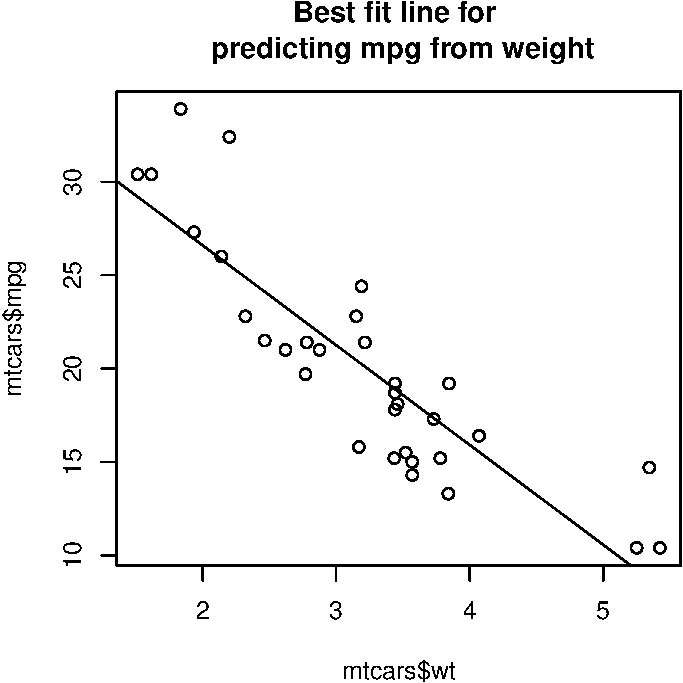
\includegraphics{visualisering_22_files/figure-latex/unnamed-chunk-45-1.pdf}

Man skriver relationen i R som \texttt{mpg\ \textasciitilde{}\ wt} og benytter \texttt{lm()}(\texttt{lm(mpg\textasciitilde{}wt,data=mtcars)}):

\begin{Shaded}
\begin{Highlighting}[]
\NormalTok{mylm }\OtherTok{\textless{}{-}} \FunctionTok{lm}\NormalTok{(mpg }\SpecialCharTok{\textasciitilde{}}\NormalTok{ wt, }\AttributeTok{data=}\NormalTok{mtcars)  }\CommentTok{\# build linear regression model}
\NormalTok{mylm}
\end{Highlighting}
\end{Shaded}

\begin{verbatim}
## 
## Call:
## lm(formula = mpg ~ wt, data = mtcars)
## 
## Coefficients:
## (Intercept)           wt  
##      37.285       -5.344
\end{verbatim}

Vores ``Coefficients'' beskriver den bedste rette linje:

\begin{itemize}
\tightlist
\item
  Skæringen (intercept): 37.285
\item
  Hældningskoefficient (slope): -5.344
\end{itemize}

Det betyder, at hvis vægten \texttt{wt} af en bil stiger med 1, så stiger \texttt{mpg} ved -5.344 (det vil sige at \texttt{mpg} reduceres med 5.344).

\hypertarget{r-squared-coefficient-of-determination}{%
\subsection{R-squared coefficient of determination}\label{r-squared-coefficient-of-determination}}

Den \(R^2\) eller ``forklaringsgraden'' (coefficeint of determination) har til formål at forklare, hvor godt vores lineær model passer til de data. For eksempel hvor meget af variansen i \texttt{mpg} forklares af variablen \texttt{wt}?

\begin{itemize}
\tightlist
\item
  Hvis det er tæt på 1 - så er der en meget tæt relation (hvis man kender vægten, så vide man også \texttt{mpg} med stor sikkerhed)
\item
  Hvis det er tæt på 0 - så er relationen svag - høj sandsynlighed for, at der er andre variabler der bedre kan forklare variansen i \texttt{mpg}.
\end{itemize}

I ovenstående model, kan man se den \(R^2\) værdi med \texttt{summary(mylm)}.

\begin{Shaded}
\begin{Highlighting}[]
\FunctionTok{summary}\NormalTok{(mylm)}
\end{Highlighting}
\end{Shaded}

\begin{verbatim}
## 
## Call:
## lm(formula = mpg ~ wt, data = mtcars)
## 
## Residuals:
##     Min      1Q  Median      3Q     Max 
## -4.5432 -2.3647 -0.1252  1.4096  6.8727 
## 
## Coefficients:
##             Estimate Std. Error t value Pr(>|t|)    
## (Intercept)  37.2851     1.8776  19.858  < 2e-16 ***
## wt           -5.3445     0.5591  -9.559 1.29e-10 ***
## ---
## Signif. codes:  0 '***' 0.001 '**' 0.01 '*' 0.05 '.' 0.1 ' ' 1
## 
## Residual standard error: 3.046 on 30 degrees of freedom
## Multiple R-squared:  0.7528, Adjusted R-squared:  0.7446 
## F-statistic: 91.38 on 1 and 30 DF,  p-value: 1.294e-10
\end{verbatim}

Det fortæller os, at \(R^2\) = 0.7528.

\hypertarget{antagelser---lineuxe6r-regression}{%
\subsection{Antagelser - lineær regression}\label{antagelser---lineuxe6r-regression}}

\begin{itemize}
\tightlist
\item
  Normalfordelte residualer
\item
  Residualer har samme spredning (varianshomogenitet)
\item
  Uafhængighed
\item
  Fit er linæer
\end{itemize}

Koden \texttt{plot(mylm,which=c(1))} angiver residualer vs predikterede (fitted) værdier - de skal være tilfældigt fordelt over plottet og prikkernes varians skal være nogenlunde konstant langt x-aksen (det giver, at den røde linje er flade).

\begin{Shaded}
\begin{Highlighting}[]
\FunctionTok{plot}\NormalTok{(mylm,}\AttributeTok{which=}\FunctionTok{c}\NormalTok{(}\DecValTok{1}\NormalTok{))}
\end{Highlighting}
\end{Shaded}

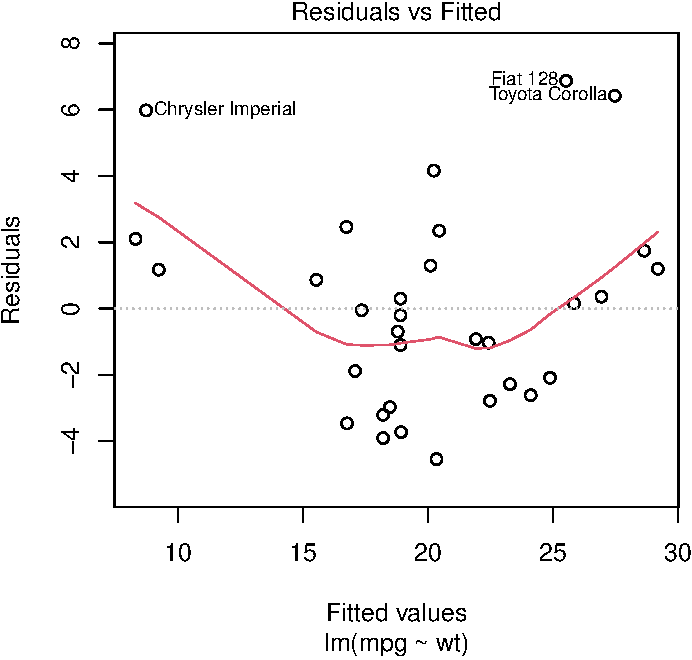
\includegraphics{visualisering_22_files/figure-latex/unnamed-chunk-48-1.pdf}

Med koden \texttt{plot(mylm,which=c(2))} kan man tjekke antagelsen på en normal fordeling. Punkterne skal være nogenlunde tæt på den diagonale linje.

\begin{Shaded}
\begin{Highlighting}[]
\FunctionTok{plot}\NormalTok{(mylm,}\AttributeTok{which=}\FunctionTok{c}\NormalTok{(}\DecValTok{2}\NormalTok{))}
\end{Highlighting}
\end{Shaded}

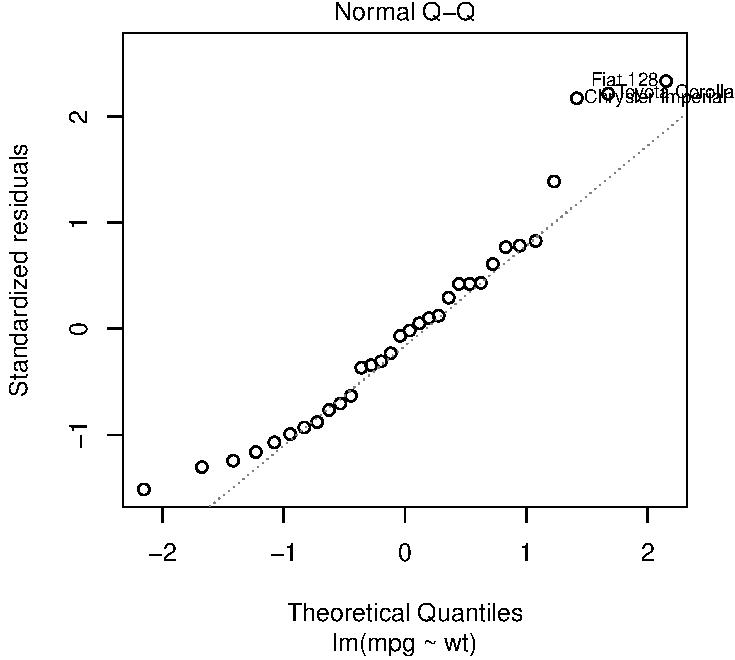
\includegraphics{visualisering_22_files/figure-latex/unnamed-chunk-49-1.pdf}

\hypertarget{multiple-lineuxe6r-regression}{%
\subsection{Multiple lineær regression}\label{multiple-lineuxe6r-regression}}

Her kan man tilføje flere variabler i vores model formel.

\begin{Shaded}
\begin{Highlighting}[]
\NormalTok{mylm\_disp }\OtherTok{\textless{}{-}} \FunctionTok{lm}\NormalTok{(mpg }\SpecialCharTok{\textasciitilde{}}\NormalTok{ wt }\SpecialCharTok{+}\NormalTok{ disp, }\AttributeTok{data=}\NormalTok{mtcars) }\CommentTok{\# build linear regression model}
\FunctionTok{summary}\NormalTok{(mylm\_disp)}
\end{Highlighting}
\end{Shaded}

\begin{verbatim}
## 
## Call:
## lm(formula = mpg ~ wt + disp, data = mtcars)
## 
## Residuals:
##     Min      1Q  Median      3Q     Max 
## -3.4087 -2.3243 -0.7683  1.7721  6.3484 
## 
## Coefficients:
##             Estimate Std. Error t value Pr(>|t|)    
## (Intercept) 34.96055    2.16454  16.151 4.91e-16 ***
## wt          -3.35082    1.16413  -2.878  0.00743 ** 
## disp        -0.01773    0.00919  -1.929  0.06362 .  
## ---
## Signif. codes:  0 '***' 0.001 '**' 0.01 '*' 0.05 '.' 0.1 ' ' 1
## 
## Residual standard error: 2.917 on 29 degrees of freedom
## Multiple R-squared:  0.7809, Adjusted R-squared:  0.7658 
## F-statistic: 51.69 on 2 and 29 DF,  p-value: 2.744e-10
\end{verbatim}

Her kan man se, at med tilføjelsen af variablen \texttt{disp}, er \(R^2\) steget til 0.7809. Bemærk, at jo flere variabler man tilføjer til modellen, jo større bliver \(R^2\)-værdien. Den adjusted \(R^2\) værdi er lavere fordi den prøver at tage højde for kompleksiteten af modellen (hvor mange parametre der er).

Variablen \texttt{disp} er faktisk ikke selv signifikant når der er taget højde for variablen \texttt{wt} (p-værdien 0.0636 - tjek, at du selv kan finde værdien i resultatet).

Hvis en af de uafhængige variabler er kategorisk bruger man funktionen \texttt{anova} til at teste den overordnet effekt af den variabel. For eksempel har variablen \texttt{cyl} 3 mulige værdier (niveauer) - 4, 6 og 8. Vi kan inddrage variablen i vores model: --\textgreater{}

\begin{Shaded}
\begin{Highlighting}[]
\NormalTok{mylm\_cyl }\OtherTok{\textless{}{-}} \FunctionTok{lm}\NormalTok{(mpg }\SpecialCharTok{\textasciitilde{}}\NormalTok{ wt }\SpecialCharTok{+} \FunctionTok{factor}\NormalTok{(cyl), }\AttributeTok{data=}\NormalTok{mtcars) }\CommentTok{\# build linear regression model}
\FunctionTok{summary}\NormalTok{(mylm\_cyl)}
\end{Highlighting}
\end{Shaded}

\begin{verbatim}
## 
## Call:
## lm(formula = mpg ~ wt + factor(cyl), data = mtcars)
## 
## Residuals:
##     Min      1Q  Median      3Q     Max 
## -4.5890 -1.2357 -0.5159  1.3845  5.7915 
## 
## Coefficients:
##              Estimate Std. Error t value Pr(>|t|)    
## (Intercept)   33.9908     1.8878  18.006  < 2e-16 ***
## wt            -3.2056     0.7539  -4.252 0.000213 ***
## factor(cyl)6  -4.2556     1.3861  -3.070 0.004718 ** 
## factor(cyl)8  -6.0709     1.6523  -3.674 0.000999 ***
## ---
## Signif. codes:  0 '***' 0.001 '**' 0.01 '*' 0.05 '.' 0.1 ' ' 1
## 
## Residual standard error: 2.557 on 28 degrees of freedom
## Multiple R-squared:  0.8374, Adjusted R-squared:   0.82 
## F-statistic: 48.08 on 3 and 28 DF,  p-value: 3.594e-11
\end{verbatim}

Man kan ikke se den overordnet effekt af \texttt{cyl} fra den ovenstående \texttt{summary} men man kan teste den med \texttt{anova}:

\begin{Shaded}
\begin{Highlighting}[]
\FunctionTok{anova}\NormalTok{(mylm,mylm\_cyl)}
\end{Highlighting}
\end{Shaded}

\begin{verbatim}
## Analysis of Variance Table
## 
## Model 1: mpg ~ wt
## Model 2: mpg ~ wt + factor(cyl)
##   Res.Df    RSS Df Sum of Sq      F   Pr(>F)   
## 1     30 278.32                                
## 2     28 183.06  2    95.263 7.2856 0.002835 **
## ---
## Signif. codes:  0 '***' 0.001 '**' 0.01 '*' 0.05 '.' 0.1 ' ' 1
\end{verbatim}

Så kan man se, at \texttt{cyl} er signifikant.

\hypertarget{problemstillinger}{%
\section{Problemstillinger}\label{problemstillinger}}

Lav quizzen og ellers vælg øvelser efter egen erfaring:

\begin{itemize}
\tightlist
\item
  2-8 er meget grundlæggende og de fleste kan springer over hvis nogenlunde tryg med base-R
\item
  9-15 anbefaler jeg til alle som en god måde at tjekke viden på
\item
  16-20 øver hvordan man andre statistiske teste i R - regression kommer jeg ind på igen senere men det hjælper hvis du er tryg med brugen af funktionen \texttt{lm} til at lave modeller i ANOVA/simpel lineær regression (se også video og problemstillingerne i morgen).
\end{itemize}

\hypertarget{quiz---basics}{%
\subsection{Quiz - Basics}\label{quiz---basics}}

\textbf{1)} Se quiz i Absalon, der hedder ``Quiz - Basics''.

\hypertarget{grundluxe6ggende-r}{%
\subsection{Grundlæggende R}\label{grundluxe6ggende-r}}

\textbf{2)} (\textbf{helt baserende viden}) Åbn en ny fil i Rstudio ved at trykke på ``File'' \textgreater{} ``New File'' \textgreater{} ``R script''. Køre følgende kode en linje ad gangen og tjek, du kan forstå outputtet.

Husk at den nemmeste måde at køre kode er ved at trykke CMD+ENTER (Mac) eller WIN-KEY+ENTER (Windows).

\begin{Shaded}
\begin{Highlighting}[]
\DecValTok{2}\SpecialCharTok{+}\DecValTok{2}
\DecValTok{2}\SpecialCharTok{*}\DecValTok{2}
\NormalTok{x }\OtherTok{\textless{}{-}} \DecValTok{4}
\NormalTok{x }\OtherTok{\textless{}{-}}\NormalTok{ x}\SpecialCharTok{+}\DecValTok{2}
\FunctionTok{sqrt}\NormalTok{(x)}
\FunctionTok{sqrt}\NormalTok{(x)}\SpecialCharTok{\^{}}\DecValTok{2}
\FunctionTok{rnorm}\NormalTok{(}\DecValTok{10}\NormalTok{,}\DecValTok{2}\NormalTok{,}\DecValTok{2}\NormalTok{)}
\FunctionTok{log10}\NormalTok{(}\DecValTok{100}\NormalTok{)}
\NormalTok{y }\OtherTok{\textless{}{-}}  \FunctionTok{c}\NormalTok{(}\DecValTok{1}\NormalTok{,}\DecValTok{4}\NormalTok{,}\DecValTok{6}\NormalTok{,}\DecValTok{4}\NormalTok{,}\DecValTok{3}\NormalTok{)}
\FunctionTok{class}\NormalTok{(y)}
\FunctionTok{class}\NormalTok{(}\FunctionTok{c}\NormalTok{(}\StringTok{"a"}\NormalTok{,}\StringTok{"b"}\NormalTok{,}\StringTok{"c"}\NormalTok{))}
\FunctionTok{mean}\NormalTok{(y)}
\FunctionTok{sd}\NormalTok{(y)}
\FunctionTok{seq}\NormalTok{(}\DecValTok{1}\NormalTok{,}\DecValTok{13}\NormalTok{,}\AttributeTok{by=}\DecValTok{3}\NormalTok{)}
\end{Highlighting}
\end{Shaded}

\textbf{3)} (\textbf{helt baserende viden}) Køre følgende kode til at åbne nogle af de indbygget datasæt, som vi bruger i kurset.
* Prøve \texttt{head()}, \texttt{nrow()}, \texttt{summary()} osv.
* Prøve også fk. \texttt{?cars} for at se en beskrivelse.

\begin{Shaded}
\begin{Highlighting}[]
\FunctionTok{data}\NormalTok{(iris)}
\FunctionTok{data}\NormalTok{(cars)}
\FunctionTok{data}\NormalTok{(ToothGrowth)}
\FunctionTok{data}\NormalTok{(sleep)}
\FunctionTok{head}\NormalTok{(chickwts)}
\FunctionTok{data}\NormalTok{(trees)}
\CommentTok{\#se her for andre:}
\FunctionTok{library}\NormalTok{(}\AttributeTok{help =} \StringTok{"datasets"}\NormalTok{)}
\end{Highlighting}
\end{Shaded}

\textbf{4)} (\textbf{baserende plots}) Jeg giver nogle muligheder for datasættet ``iris''. Afprøve funktionerne for nogle af de andre ovenstående indbygget datasæt, som du indlæst.

\begin{Shaded}
\begin{Highlighting}[]
\FunctionTok{plot}\NormalTok{(iris}\SpecialCharTok{$}\NormalTok{Sepal.Length,iris}\SpecialCharTok{$}\NormalTok{Sepal.Width)}
\FunctionTok{hist}\NormalTok{(iris}\SpecialCharTok{$}\NormalTok{Sepal.Width)}
\FunctionTok{boxplot}\NormalTok{(iris}\SpecialCharTok{$}\NormalTok{Sepal.Length}\SpecialCharTok{\textasciitilde{}}\NormalTok{iris}\SpecialCharTok{$}\NormalTok{Species)}
\end{Highlighting}
\end{Shaded}

Man kan også gøre plotterne lidt pænere ved at give dem en titel/aksen-navne osv. Prøve \texttt{?plot} for at se nogle muligheder, og tilføje \texttt{ylab}, \texttt{xlab}, \texttt{main} (titel) i én af plotterne. Leg også med \texttt{col} (farver). Bemærk dog, at vi kommer til at ændre måden at lave plotter på når vi starter \texttt{ggplot2}.

\textbf{5)} (\textbf{dataframes}) Brug datasættet \texttt{cars} (\texttt{data(cars)}) til at:

\begin{itemize}
\tightlist
\item
  Lav et scatter plot med speed på x-aksen og dist på y-aksen
\item
  Tilføj en ny kolon med følgende kode:
\end{itemize}

\begin{Shaded}
\begin{Highlighting}[]
\NormalTok{cars}\SpecialCharTok{$}\NormalTok{fast }\OtherTok{\textless{}{-}}\NormalTok{ cars}\SpecialCharTok{$}\NormalTok{speed}\SpecialCharTok{\textgreater{}}\DecValTok{15}
\end{Highlighting}
\end{Shaded}

\begin{itemize}
\tightlist
\item
  Brug \texttt{mean} på den nye variabel til at finde ud af proportionen af biler, der er hurtige
\item
  Beregn gennemsnitsværdien af variablen \texttt{dist} for hurtige biler og ikke-hurtige biler hver for sig (brug funktionen \texttt{tapply}). Gem resultatet med \texttt{\textless{}-}.
\item
  Brug \texttt{barplot} til at lave et plot af den gennemsnitlige \texttt{dist} for hurtige og ikke-hurtige biler.
\end{itemize}

\textbf{6)} (\textbf{dataframes}) Lav en ny dataframe (funktionen \texttt{data.frame()}) med tre kolonner som hedder ``navn'', ``alder'' og ``yndlings\_farve'' (find bare selv på værdierne). Sørge for, at den har 4 rækker.

\begin{Shaded}
\begin{Highlighting}[]
\NormalTok{mydf }\OtherTok{\textless{}{-}} \FunctionTok{data.frame}\NormalTok{(}\StringTok{"navn"}\OtherTok{=} \FunctionTok{c}\NormalTok{(}\StringTok{"alice"}\NormalTok{,}\StringTok{"freddy"}\NormalTok{, ... ), }\StringTok{"alder"} \OtherTok{=} \FunctionTok{c}\NormalTok{(...), ...) }\CommentTok{\#not run, slette "..." og skrive videre}
\FunctionTok{dim}\NormalTok{(mydf) }\CommentTok{\# fire række og tre kolonner}
\NormalTok{mydf}
\end{Highlighting}
\end{Shaded}

\textbf{7)} (\textbf{dataframes}) Tilføj en ny variabel \texttt{random} til ovenstående dataframe, hvor værdierne kommer fra en normal fordeling med et gennemsnit på 5 og sd på 1 (bruge funktionen \texttt{rnorm}).

\begin{Shaded}
\begin{Highlighting}[]
\NormalTok{mydf}\SpecialCharTok{$}\NormalTok{random }\OtherTok{\textless{}{-}} \CommentTok{\#??}
\end{Highlighting}
\end{Shaded}

\textbf{8)} (\textbf{delmængder af dataframes}) Åbn datasættet ``ToothGrowth'' med følgende kode:

\begin{Shaded}
\begin{Highlighting}[]
\FunctionTok{data}\NormalTok{(}\StringTok{"ToothGrowth"}\NormalTok{)}
\NormalTok{?ToothGrowth}
\end{Highlighting}
\end{Shaded}

\begin{itemize}
\tightlist
\item
  Find delmængden af datasættet således at diet (variablen \texttt{supp}) er ``OJ'' og længden (variablen \texttt{len}) er større end 15.
\end{itemize}

\begin{Shaded}
\begin{Highlighting}[]
\NormalTok{newdf }\OtherTok{\textless{}{-}}\NormalTok{ ToothGrowth[}\CommentTok{\#skrive her til at lave subset af observationerne,]}
\end{Highlighting}
\end{Shaded}

\begin{itemize}
\tightlist
\item
  Hvor mange rækker er der i den nye dataframe \texttt{newdf}?
\item
  Hvor mange unikke værdier er der i variablen \texttt{dose} (brug funktionen \texttt{unique}) ?
\item
  Find delmængden af datasættet \texttt{ToothGrowth}, hvor variablen \texttt{dose} er 0.5 eller 1.5 (hint: brug \texttt{\%in\%} eller \texttt{\textbar{}}) og \texttt{supp} er ``VC''.
\item
  Beregn den gennemsnitlige længde for observationerne i delmængden.
\end{itemize}

\hypertarget{kort-analyse-med-reaktionstider}{%
\subsection{Kort analyse med reaktionstider}\label{kort-analyse-med-reaktionstider}}

\textbf{9)} (\textbf{indlæse data}) Åbn en fil, der sidder i Absalon og hedder ``reactions.txt'' ved at bruge funktionen \texttt{read.table()} (kalde det for \texttt{data}). Husk at tjekke, om selve filen har variabelnavne og bruge således \texttt{header=T} hvis nødvendigt.

\begin{Shaded}
\begin{Highlighting}[]
\NormalTok{data }\OtherTok{\textless{}{-}}\NormalTok{ ... }\CommentTok{\#replace ...}
\end{Highlighting}
\end{Shaded}

\textbf{10)} (\textbf{factor variabler}) Variablerne \texttt{subject} og \texttt{time} indlæses som henholdvis data type `int' (heltal) og ``chr'' (character) men de skal hellere være `factor' variabler. Lav dem om til facktor variabler.

\begin{Shaded}
\begin{Highlighting}[]
\CommentTok{\#gør subject til en faktor}
\NormalTok{data}\SpecialCharTok{$}\NormalTok{subject }\OtherTok{\textless{}{-}} \FunctionTok{as.factor}\NormalTok{(data}\SpecialCharTok{$}\NormalTok{subject) }

\DocumentationTok{\#\# gør den samme her for time:}
\end{Highlighting}
\end{Shaded}

\begin{itemize}
\tightlist
\item
  Hvor mange niveauer er der i hver af de to variabler?
\end{itemize}

\textbf{11)} (\textbf{delmængde af dataframe})

Lav to delmængder af ovenstående datasæt -

\begin{itemize}
\tightlist
\item
  én til alle observationer fra tidspunktet ``before'' (brug koden \texttt{data\$time\ =="before"} til at udvælge rækkerne fra dataframe) og
\item
  én til alle observationer fra tidspunktet ``after''.
\end{itemize}

\begin{Shaded}
\begin{Highlighting}[]
\NormalTok{RT\_before }\OtherTok{\textless{}{-}}\NormalTok{ data[}\CommentTok{\#skrive her , ]}
\NormalTok{RT\_after }\OtherTok{\textless{}{-}} \CommentTok{\#skrive her}
\end{Highlighting}
\end{Shaded}

\begin{itemize}
\tightlist
\item
  Brug \texttt{RT\_before} og lav en delmængde der viser alle observationer fra tidspunktet ``before'' med en rekationstid af mindst 800.

  \begin{itemize}
  \tightlist
  \item
    Hvor mange personer opfylder kriteren?
  \end{itemize}
\end{itemize}

\begin{Shaded}
\begin{Highlighting}[]
\NormalTok{RT\_before\_mindst800 }\OtherTok{\textless{}{-}} \CommentTok{\#skrive her}
\end{Highlighting}
\end{Shaded}

\textbf{12)} (\textbf{mean og tapply}) Benyt funktionen \texttt{mean} til at beregne den gennemsnitlige reaktionstid (variablen \texttt{RT}) til ``before'' og ``after'' hver for sig (brug ovenstående delmængder).

\begin{itemize}
\tightlist
\item
  Prøv også at anvende funktionen \texttt{tapply} på det oprindelige datasæt \texttt{data} til at beregene samme middelværdi med mindre kode.
\end{itemize}

\begin{Shaded}
\begin{Highlighting}[]
\FunctionTok{tapply}\NormalTok{(}\CommentTok{\#skrive her,\#skrive her,\#skrive her)}
\end{Highlighting}
\end{Shaded}

\begin{itemize}
\tightlist
\item
  Er reaktionstiderne blevet hurtigere eller langsommere i gennemsnit?
\end{itemize}

\textbf{13)} (\textbf{beregn forskellen og mean})

Bemærk, at datasættet er `paired' - målingerne er lavet på de præcis samme personer både ``before'' og ``after''.

\begin{itemize}
\tightlist
\item
  Opret en vector \texttt{diff}, der er ændringen i reaktionstiderne mellem personerne ``before'' og ``after''.
\item
  Beregn den gennemsnitlige forskel i rekationstiderne.
\end{itemize}

\begin{Shaded}
\begin{Highlighting}[]
\NormalTok{diff }\OtherTok{\textless{}{-}} \CommentTok{\#change in reaction time between before and after}
\FunctionTok{mean}\NormalTok{(diff)}
\end{Highlighting}
\end{Shaded}

\begin{itemize}
\tightlist
\item
  Tjek tegnet stemmer overens med din konklusion fra \textbf{11)} - hvis den er positiv, så betyder det, at reaktionstiderne er blevet langsommere.
\end{itemize}

\textbf{14)} (\textbf{lav t-test i R}) Lav en t-test (funktionen \texttt{t.test}) for at teste hypotesen at den gennemsnitslige forskel i reaktionstiderne mellem ``before'' og ``after'' er anderledes end 0.

\begin{Shaded}
\begin{Highlighting}[]
\FunctionTok{t.test}\NormalTok{(}\CommentTok{\#skrive her..)}
\end{Highlighting}
\end{Shaded}

Find følgende i outputtet fra R:

\begin{itemize}
\tightlist
\item
  Hvor er test-statistik \texttt{t}?
\item
  Hvor er p-værdien?
\item
  Hvad er alternativhypotesen?
\end{itemize}

\textbf{15)} Skriv en kort sætning med din konklusion.

\hypertarget{ekstra-uxf8velser-med-statistik-tests}{%
\subsection{Ekstra øvelser med statistik tests}\label{ekstra-uxf8velser-med-statistik-tests}}

\textbf{16)} (\textbf{Chi-sq}) Kør følgende kode til at få en tabel (selve koden er ikke vigtigt):

\begin{Shaded}
\begin{Highlighting}[]
\NormalTok{mytable }\OtherTok{\textless{}{-}} \FunctionTok{structure}\NormalTok{(}\FunctionTok{c}\NormalTok{(80L, 97L, 372L, 136L, 87L, 119L), }\AttributeTok{.Dim =} \DecValTok{3}\SpecialCharTok{:}\DecValTok{2}\NormalTok{, }\AttributeTok{.Dimnames =} \FunctionTok{structure}\NormalTok{(}\FunctionTok{list}\NormalTok{(}
    \FunctionTok{c}\NormalTok{(}\StringTok{"First"}\NormalTok{, }\StringTok{"Second"}\NormalTok{, }\StringTok{"Third"}\NormalTok{), }\FunctionTok{c}\NormalTok{(}\StringTok{"Died"}\NormalTok{, }\StringTok{"Survived"}\NormalTok{)), }\AttributeTok{.Names =} \FunctionTok{c}\NormalTok{(}\StringTok{"Class"}\NormalTok{, }\StringTok{"Survival"}\NormalTok{)), }\AttributeTok{class =} \StringTok{"table"}\NormalTok{)}

\NormalTok{mytable}
\end{Highlighting}
\end{Shaded}

\begin{verbatim}
##         Survival
## Class    Died Survived
##   First    80      136
##   Second   97       87
##   Third   372      119
\end{verbatim}

Tabellen omhandler personer ombord skibet `Titanic' (der sank den 15. april 1912 efter et sammenstød med et isbjerg 600 km sydøst for Halifax, Nova Scotia i Canada). Tabellen angiver hvor mange passagerer tilhørte de tre klass (førsteklass, andenklass, trejdeklass), delte efter overlevelsesudfald (døde eller overlevede tragedien).

\begin{itemize}
\item
  Benyt funktionen \texttt{chisq.test()} på tabellen.
\item
  Hvad er nulhypotesen?

  \begin{itemize}
  \tightlist
  \item
    Overlevelsesudfald er uafhængig af klass
  \end{itemize}
\item
  Er testen signifikant?

  \begin{itemize}
  \tightlist
  \item
    p-value \textless{} 2.2e-16 - ja
  \end{itemize}
\item
  Er passagerernes klass så uafhængige af deres chance for at overleve tragedien?

  \begin{itemize}
  \tightlist
  \item
    Jeg forkaster nulhypotesen og konkluderer de to variabler afhængige af hinanden
  \end{itemize}
\item
  Hvilken klass havde den bedste chance for at overleve?

  \begin{itemize}
  \tightlist
  \item
    Førsteklass = meget højere chance
  \end{itemize}
\end{itemize}

Vi kommer til at arbejde meget mere med datasættet \texttt{Titanic} i emnet Tidyverse - dag 1!

\textbf{17)} (\textbf{Korrelation analyse}) Åbn datasættet \texttt{trees} og lav et scatter plot med variablen \texttt{Girth} på x-aksen og variablen \texttt{Volume} på y-aksen.

\begin{Shaded}
\begin{Highlighting}[]
\FunctionTok{data}\NormalTok{(trees)}
\FunctionTok{summary}\NormalTok{(trees)}
\end{Highlighting}
\end{Shaded}

\begin{itemize}
\tightlist
\item
  Anvend funktionen \texttt{cor.test} for at teste, om der er en signifikant korrelation mellem de to variabler. Brug \texttt{method\ =\ "pearson"} (det er dog faktisk default)
\end{itemize}

\begin{Shaded}
\begin{Highlighting}[]
\FunctionTok{cor.test}\NormalTok{(???, ???,}\AttributeTok{method=}\StringTok{"pearson"}\NormalTok{)}
\end{Highlighting}
\end{Shaded}

\begin{itemize}
\tightlist
\item
  Hvad er korrelationen mellem \texttt{Girth} og \texttt{Volume}?
\item
  Hvad er p-værdien? Er den signifikant?
\end{itemize}

\textbf{18)} (\textbf{ANOVA}) OBS: hvis du føler dig utryg med funktionen \texttt{lm()} - der kommer en video om det i morgen (i forbindelse med emnet Rmarkdown).

Kør følgende kode til at lave variansanalyse, der tester hulhypotesen hvor den gennemsnitlige værdi af variablen \texttt{Sepal.Width} er ens for hver af de tre arter (variablen \texttt{Species}) fra datasættet \texttt{iris}:

\begin{Shaded}
\begin{Highlighting}[]
\FunctionTok{data}\NormalTok{(iris)}

\CommentTok{\#model under H0: no difference according to group variable Species (1 just means "fit overall mean")}
\NormalTok{model\_h0 }\OtherTok{\textless{}{-}} \FunctionTok{lm}\NormalTok{(Sepal.Width }\SpecialCharTok{\textasciitilde{}} \DecValTok{1}\NormalTok{, }\AttributeTok{data=}\NormalTok{iris) }

\CommentTok{\#model under H1: each level of group variable Species has its own mean}
\NormalTok{model\_h1 }\OtherTok{\textless{}{-}} \FunctionTok{lm}\NormalTok{(Sepal.Width }\SpecialCharTok{\textasciitilde{}}\NormalTok{ Species, }\AttributeTok{data=}\NormalTok{iris) }

\CommentTok{\#compare two models {-} significant p{-}value equates to choosing H1 model}
\FunctionTok{anova}\NormalTok{(model\_h0,model\_h1)}
\end{Highlighting}
\end{Shaded}

\begin{verbatim}
## Analysis of Variance Table
## 
## Model 1: Sepal.Width ~ 1
## Model 2: Sepal.Width ~ Species
##   Res.Df    RSS Df Sum of Sq     F    Pr(>F)    
## 1    149 28.307                                 
## 2    147 16.962  2    11.345 49.16 < 2.2e-16 ***
## ---
## Signif. codes:  0 '***' 0.001 '**' 0.01 '*' 0.05 '.' 0.1 ' ' 1
\end{verbatim}

Kig på outputtet:

\begin{itemize}
\tightlist
\item
  Hvilken model reflekterer nulhypotesen?
\item
  Hvilken model reflekterer alternativhypotesen?
\item
  Hvor er p-værdien?
\item
  Er der en signifikant forskel i den gennemsnitlige \texttt{Sepal.Width} efter de forskellige \texttt{Species}?
\end{itemize}

Brug funktionen \texttt{tapply} for at finde ud af, hvad er den middelværdi \texttt{Sepal.Width} til hver af de tre arter.

\textbf{19)} (\textbf{ANOVA}) Lav en lignende analyse på datasættet \texttt{chickwts} for at svare på spørgsmålet:

\begin{itemize}
\tightlist
\item
  Er der en forskel i den gennemsnitlige vægt (variablen \texttt{weight}) efter fodertypen (variablen \texttt{feed})? Med andre ord er vægt afhængig af fodertypen?
\end{itemize}

\begin{Shaded}
\begin{Highlighting}[]
\FunctionTok{data}\NormalTok{(chickwts)}
\end{Highlighting}
\end{Shaded}

\textbf{Valgfri - vi gennemgår også lineær regression i morgen og du kan altid komme tilbage senere hvis du har bruge for det}

\textbf{20)} (\textbf{Lineær regression})

\begin{itemize}
\tightlist
\item
  Brug \texttt{lm} til at lave en simpel lineær regression, således at respons variablen \texttt{Volume} er afhængig af variablen \texttt{Girth} (datasæstet \texttt{trees}).
\end{itemize}

\begin{Shaded}
\begin{Highlighting}[]
\NormalTok{mylm }\OtherTok{\textless{}{-}} \FunctionTok{lm}\NormalTok{(???, }\AttributeTok{data=}\NormalTok{trees) }
\end{Highlighting}
\end{Shaded}

Brug \texttt{summary} på din model for at finde følgende værdier:

\begin{itemize}
\tightlist
\item
  Hvad er r.squared? (multiple)
\item
  Er variablen \texttt{Girth} signifikant?
\item
  Hvad er ligningen på den bedste rette linje (husk formen y = ax + b)?
\end{itemize}

\textbf{21)} (\textbf{Kort intro til multiple lineær regression}) Tag ovenstående model og tilføj variablen \texttt{Height} som en ekstra prediktær (uafhængig) variabel i modellen med en ``+'' tegn:

\begin{Shaded}
\begin{Highlighting}[]
\NormalTok{mylm\_height }\OtherTok{\textless{}{-}} \FunctionTok{lm}\NormalTok{(??? }\SpecialCharTok{\textasciitilde{}}\NormalTok{ ??? }\SpecialCharTok{+}\NormalTok{ ???, }\AttributeTok{data=}\NormalTok{trees) }
\FunctionTok{summary}\NormalTok{(mylm\_height)}
\end{Highlighting}
\end{Shaded}

\emph{Bemærk at det ikke betyder, at de to variabler skal lægges sammen, men at vi gerne vil have både variablerne i modellen som uafhængig variabler (med andre ord er \texttt{Volume} afhængig af både \texttt{Girth} og \texttt{Height}).}

Benyt \texttt{summary} på modellen og prøv at finde følgende:

\begin{itemize}
\tightlist
\item
  Hvad er den den (multiple) r.squared værdi?
\item
  Hvor meget ændre den (multiple) r.squared værdi i forhold til modellen med kun variablen \texttt{Girth}?
\item
  Er \texttt{Volume} signifikant afhængig af \texttt{Height} (efter at man har taget højde for \texttt{Girth})?
\end{itemize}

Brug funktionen \texttt{anova} til at sammenligne modellen uden \texttt{Height} med modellen med \texttt{Height}

\begin{Shaded}
\begin{Highlighting}[]
\FunctionTok{anova}\NormalTok{(}\CommentTok{\#model without height,\#model with height)}
\end{Highlighting}
\end{Shaded}

Bemærk, at i dette tilfælde er p-værdien fra ANOVA samme p-værdi fra \texttt{summary(mylm\_height)}.

\hypertarget{rmarkdown}{%
\chapter{Introduktion til R Markdown}\label{rmarkdown}}

I dag begynder vi at arbejde med R Markdown. Selve emnet er relativt kort og er designet til, at du kan komme i gang med at bruge R Markdown i praksis, men notaterne referere også til nogle ekstra muligheder så du kan indrette dit dokument efter eget ønske. Der er to videoer - én er en `quick-start guide' for at komme i gang, og den anden viser en simpel lineær regression i R Markdown - har du ikke brug for lidt genopfriskning, kan man også se mere om funktionaliten i R Markdown.

Efter quizzerne og problemstillinger er der en worksheet, hvor du kan øve dig videre med de typer opgaver vi kommer til at se i workshopperne. Fra næste gang (fredag) skifter vi emnet til visualiseringer i \textbf{ggplot2}, og vi arbejder naturligvis i R Markdown fremadrettet.

\hypertarget{hvad-er-r-markdown}{%
\section{Hvad er R Markdown?}\label{hvad-er-r-markdown}}

R Markdown er både en nem og fleksibel måde at arbejde med R til projekter på. Her kan du kombinere din R-kode, output og tekst i samme dokument, og derudover fremviser et pænt HTML dokument fra det, som potentielt kan deles med andre. Jeg anbefaler at du bruger R Markdown til alle opgaverne i kurset og \textbf{ved eksamen forventer jeg at du afleverer et HTML dokument} til mig med din ``knittede'' kode fra din analyse.

\hypertarget{installere-r-markdown}{%
\section{Installere R Markdown}\label{installere-r-markdown}}

R Markdown er, ligesom R, gratis og `open source'. Den fungerer indenfor RStudio and kan installeres ved at bruge den følgende kommando:

\begin{Shaded}
\begin{Highlighting}[]
\FunctionTok{install.packages}\NormalTok{(}\StringTok{"rmarkdown"}\NormalTok{)}
\end{Highlighting}
\end{Shaded}

\hypertarget{videodemonstrationer}{%
\section{Videodemonstrationer}\label{videodemonstrationer}}

Jeg har lavet to videoer som kan ses her:

Video 1:

Jeg viser

\begin{itemize}
\tightlist
\item
  hvordan man laver et nyt dokument i R Markdown
\item
  hvordan man skriver tekst ind i dokumentet
\item
  hvordan man bruger ``knit'' til at lave et HTML-dokument
\item
  hvordan man opretter og kører kode chunks
\end{itemize}

Link her hvis det ikke virker nedenunder: \url{https://vimeo.com/702416505}

Video 2:

Jeg viser en kort lineær regression analyse:

\begin{itemize}
\tightlist
\item
  Indlæse datasæt og lave plot af datasættet
\item
  Lynhurtig gennemgåelse af ligningen for rette linje
\item
  Hvordan man anvender funktionen \texttt{lm()} til at fitte en lineær model
\item
  Fortolkelse af resultaterne
\end{itemize}

Link her hvis det ikke virker nedenunder: \url{https://vimeo.com/701240044}

\hypertarget{oprette-et-nyt-dokument-i-r-markdown}{%
\section{Oprette et nyt dokument i R Markdown}\label{oprette-et-nyt-dokument-i-r-markdown}}

Man åbner et nyt rmarkdown dokument ved at trykke ``New'' \textgreater{} ``New File'' \textgreater{} ``New R Markdown\ldots{}''. Man kan også trykke på ``+'' knappen øverst til venstre hjørne.

\begin{figure}
\centering
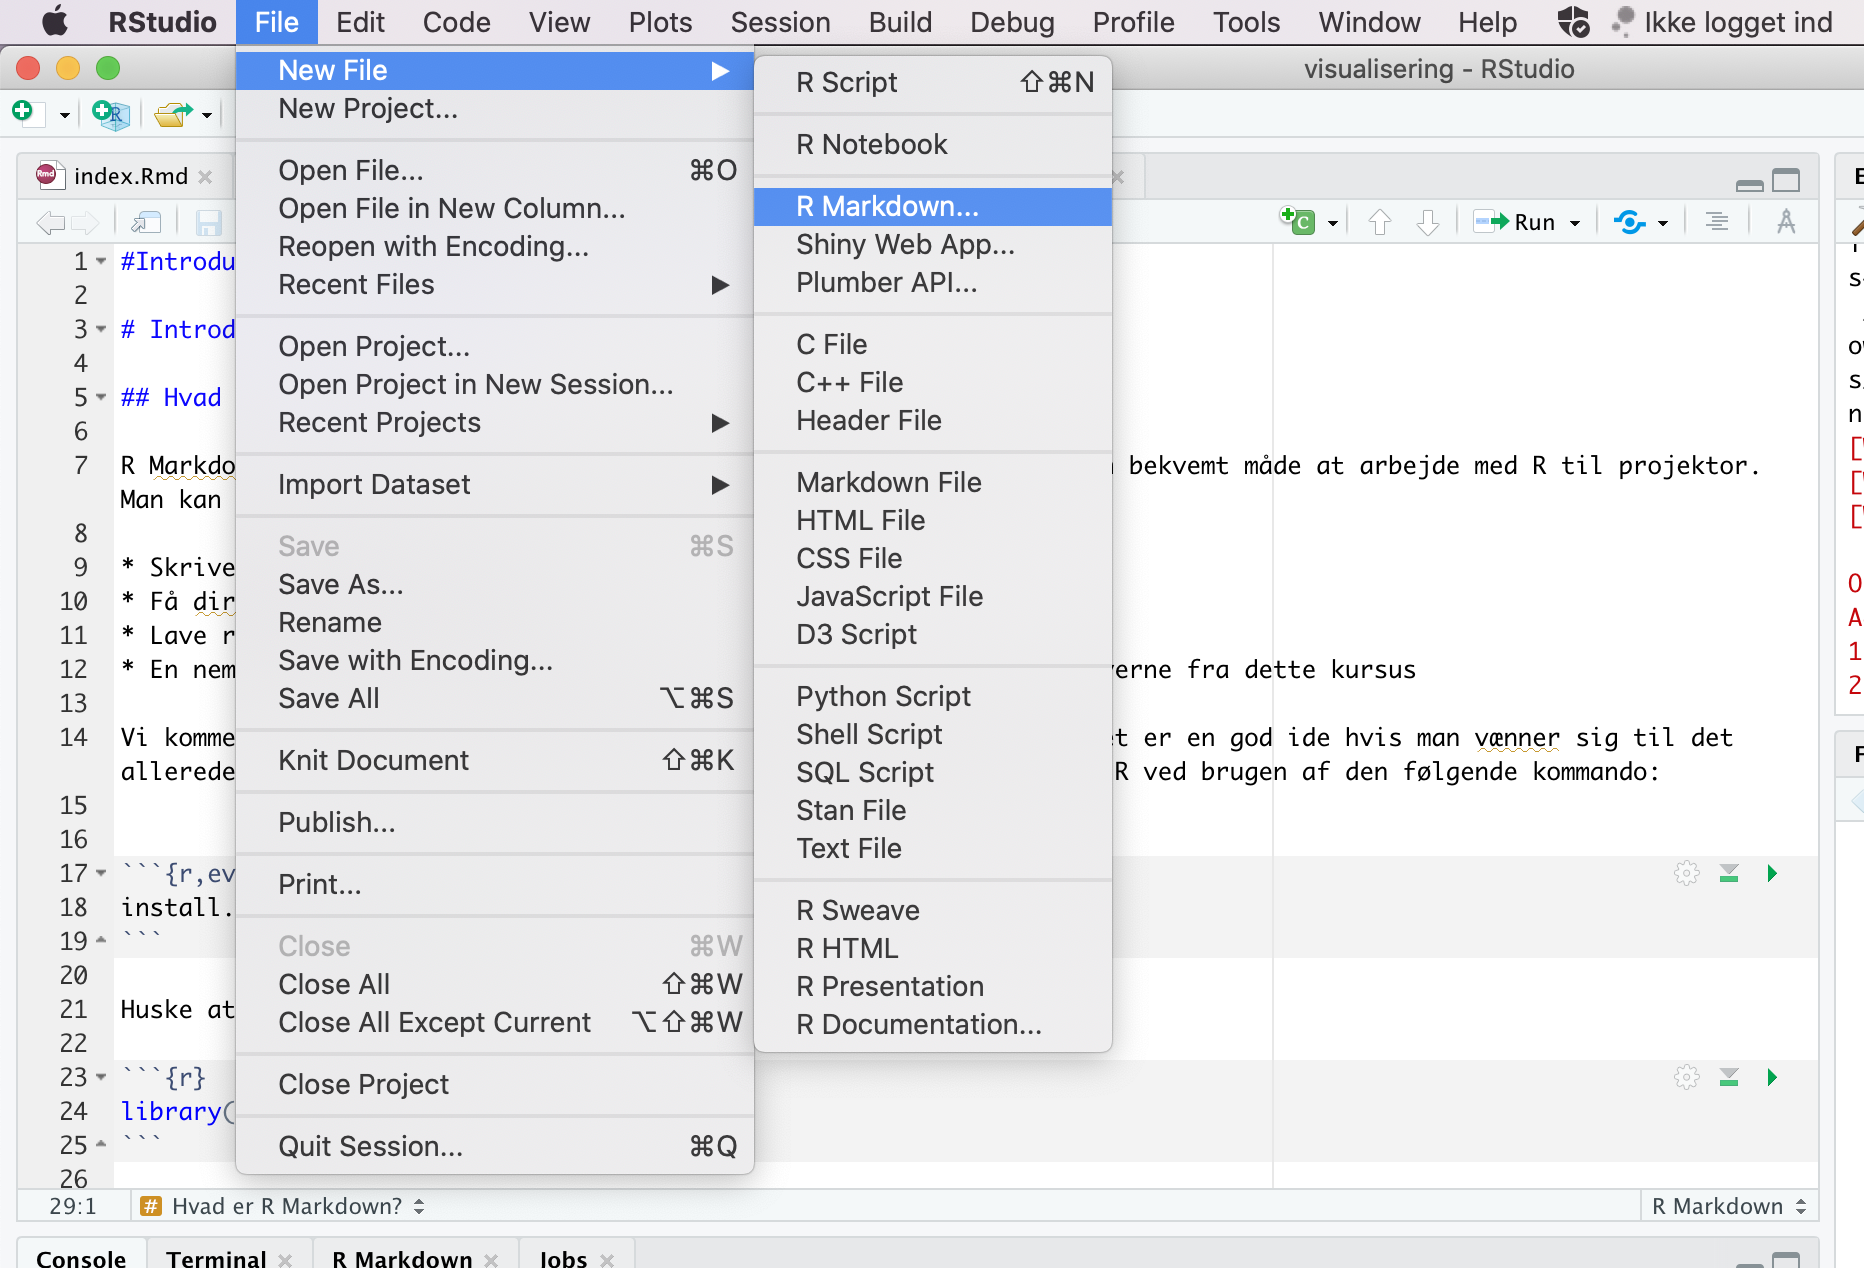
\includegraphics{plots/open_new_rmarkdown.png}
\caption{Hvordan man åbner et nyt R Markdown dokument}
\end{figure}

Dernæst angiver man en titel (det kan ændres senere hvis der er bruge for det) og bekræfter, at outputtet kommer i HTML form. I kurset arbejdes der kun med HTML dokumenter, men man har også andre muligheder, som du er velkommen til at afprøve (PDF/Word/Shiny osv\ldots).

\begin{figure}
\centering
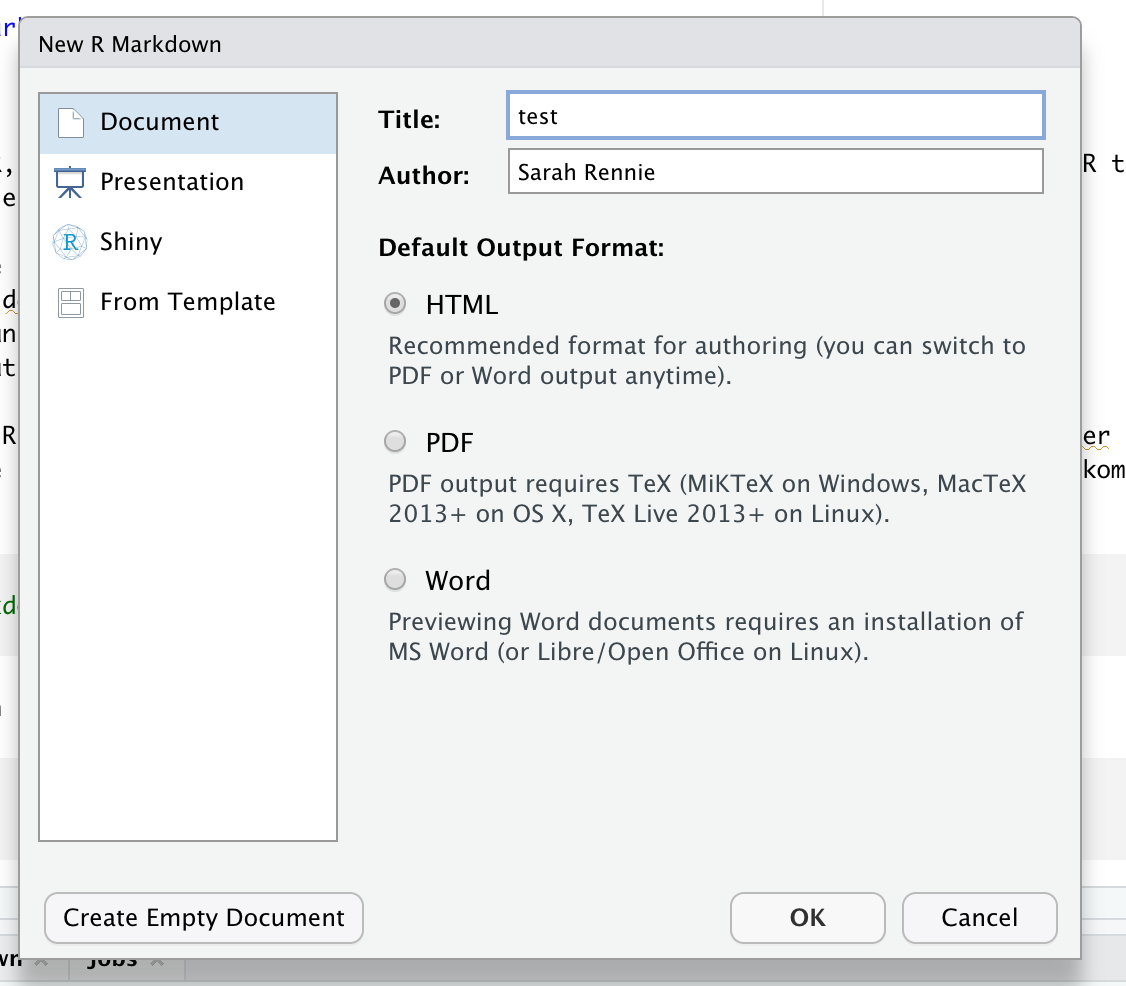
\includegraphics{plots/create_new_rmarkdown.png}
\caption{Hvordan man åbne et nyt R Markdown dokument}
\end{figure}

\hypertarget{yaml}{%
\subsection{YAML}\label{yaml}}

Den første sektion af dokument skrives i hvad der kaldes for `YAML'. (Dette står for `YAML Ain't Markup Language').

\begin{figure}
\centering
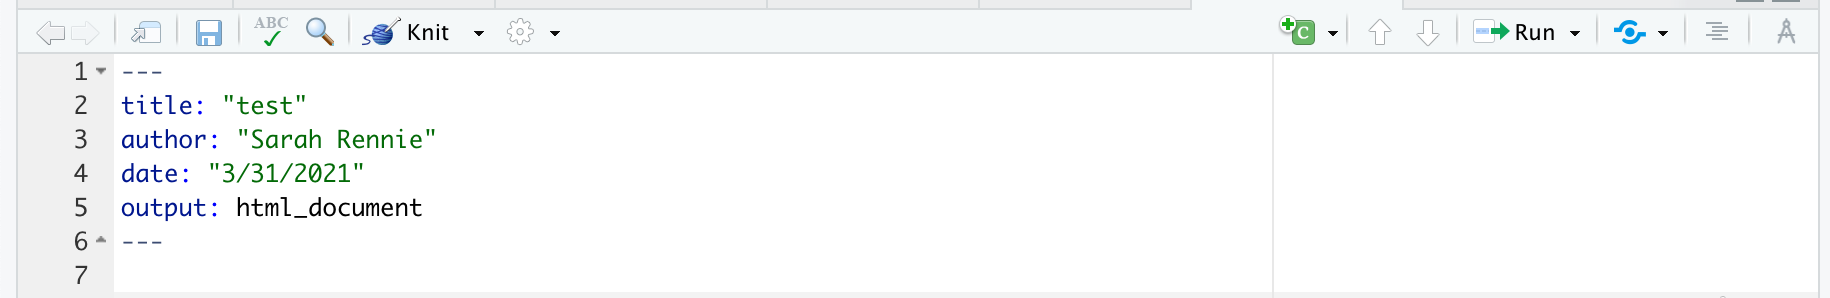
\includegraphics{plots/YAML.png}
\caption{Hvordan man åbner et nyt R Markdown dokument}
\end{figure}

Det indeholder oplysninger om dokumentet, og her kan man specificere forskellige muligheder - fk. titel, forfatter, output-type (fks. HTML eller PDF), dato, osv. I de fleste tilfælde nøjes vi med at bruge standard indstillinger, men hvis man gerne vil lære mere om de forskellige muligheder med YAML, kan man læse her:

\url{https://bookdown.org/yihui/rmarkdown/html-document.html}

eller se en liste af muligheder her på dette cheatsheet:

\url{https://www.rstudio.com/wp-content/uploads/2016/03/rmarkdown-cheatsheet-2.0.pdf}

\hypertarget{globale-options}{%
\subsection{Globale options}\label{globale-options}}

Der er også tekst som ser ud som følgende:

\begin{figure}
\centering
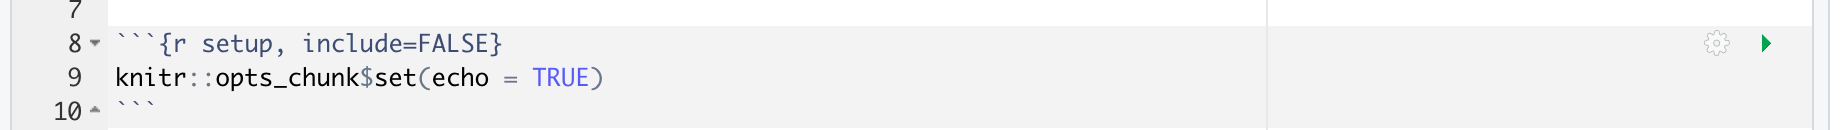
\includegraphics{plots/global_options.png}
\caption{Hvordan man åbner et nyt R Markdown dokument}
\end{figure}

Med funktionen \texttt{opts\_chunk\$set()} kan man specificere de globale indstillinger, som styrer hvordan det færdige dokument ser ud. I dette tilfælde er de fleste parametre angivet som `default' (da de ikke er nævnt eksplicit), og \texttt{echo} er den eneste der har noget angivet. Hvis \texttt{echo} er \texttt{TRUE}, så betyder det, at når man ``knitter'' sin kode (processen, der få et HTML dokument frem, se nedenfor), så kan man også se koden, der blev kørt, samt dens output, i det færdige HTML dokument, der kommmer frem.

\hypertarget{skrive-baseret-tekst}{%
\section{Skrive baseret tekst}\label{skrive-baseret-tekst}}

Her er nogle brugbare muligheder for at skrive tekst i opgaverne eller rapporter:

\begin{Shaded}
\begin{Highlighting}[]
\SpecialCharTok{*}\NormalTok{italic}\SpecialCharTok{*}   \ErrorTok{**}\NormalTok{bold}\SpecialCharTok{**}

\NormalTok{\_italic\_   \_\_bold\_\_}
\end{Highlighting}
\end{Shaded}

\emph{italic} \textbf{bold}

\emph{italic} \textbf{bold}

\hypertarget{headers}{%
\subsection{Headers}\label{headers}}

Man kan også lave sektioner:

\begin{Shaded}
\begin{Highlighting}[]
\CommentTok{\# Header 1}

\DocumentationTok{\#\# Header 2}

\DocumentationTok{\#\#\# Header 3}
\end{Highlighting}
\end{Shaded}

\begin{figure}
\centering
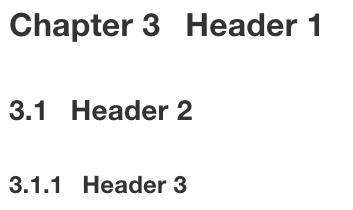
\includegraphics{header_eksempel.png}
\caption{Caption for the picture.}
\end{figure}

\hypertarget{liste}{%
\subsection{liste}\label{liste}}

\begin{Shaded}
\begin{Highlighting}[]
\SpecialCharTok{*}\NormalTok{ Item }\DecValTok{1}
\SpecialCharTok{*}\NormalTok{ Item }\DecValTok{2}
    \SpecialCharTok{+}\NormalTok{ Item 2a}
    \SpecialCharTok{+}\NormalTok{ Item 2b}
\end{Highlighting}
\end{Shaded}

\begin{itemize}
\tightlist
\item
  Item 1
\item
  Item 2

  \begin{itemize}
  \tightlist
  \item
    Item 2a
  \item
    Item 2b
  \end{itemize}
\end{itemize}

\hypertarget{knitte-kode}{%
\section{Knitte kode}\label{knitte-kode}}

Man bruger \emph{Knit} for at gengive filen i HTML form. Når man trykker på knappen \emph{Knit}, bliver samtlige koder i filen kørt og et HTML dokument fremvises. Bemærk, at \textbf{koderne bliver kørt på ny hver gang man knitter}, uden hensyn til hvad du har i din nuværende workspace i RStudio. Det betyder, at hvis du eksempelvis har pakken \texttt{tidyverse} indlæst på din computer men har glemt at skrive \texttt{library(tidyverse)} eksplicit på toppen af dit dokument, så får du en fejlmeddelelse hvis du bruger tidyverse-baserede funktioner nogle steder.

\hypertarget{kode-chunks}{%
\section{Kode chunks}\label{kode-chunks}}

Man skriver selve R kode indenfor hvad der kaldes for ``chunks''. Man kan oprette en ny chunk på flere måder - enten ved at trykke på den \emph{Insert a new code chunk} knap ovenpå, eller ved at trykke \emph{Cmd+Option+I} på tastaturet (hvis man bruger MAC) eller \emph{Ctrl+Alt+I} (hvis man bruger Windows). Det er værd at huske den keyboard-shortcut - det sparer meget tid efter egen erfaring!

Her er et eksempel af en chunk:

\begin{Shaded}
\begin{Highlighting}[]
\CommentTok{\# This is a chunk, let\textquotesingle{}s write som R code}
\NormalTok{x }\OtherTok{\textless{}{-}} \DecValTok{1}
\NormalTok{x }\SpecialCharTok{+} \DecValTok{1}
\end{Highlighting}
\end{Shaded}

\begin{verbatim}
## [1] 2
\end{verbatim}

For at køre en chunk, trykker man på den grønne pile øverste i højre hjørne på selve chunk (der hedder \emph{Run Current Chunk} når du holder musen over den). Resultatet kan ses lige nedenunder, som i ovenstående.

Bemærk, at når du arbejde med dit R Markdown dokument er det generelt hurtigere at bruge den grønne pile / \emph{Run Current Chunk} i stedet for at knitte hele dokumentet hver gang man vil køre kode. Det er fordi her kører man kun den enkel chunk i stedet for hele dokumentet på ny (herunder indlæsning af pakker og eventuelle store filer), som er tilfældet med \emph{Knit}.

\hypertarget{et-godt-ruxe5d-nuxe5r-man-arbejder-med-chunks}{%
\subsection{Et godt råd når man arbejder med chunks}\label{et-godt-ruxe5d-nuxe5r-man-arbejder-med-chunks}}

Til længere opgaver er det god praksis at sikre jævnligt, at man kan få et HTML dokument frem ved at knitte, selvom du kører din chunks lokalt mens du udvikler din kode - det vil sige, at du ikke få en alvorlig fejlmeddelelse, der forhindre din koder at knitte. \textbf{Det er dit ansvar at sikre, at din kode fungerer som helhed og du kan dermed producere et HTML dokument med din løsninger.}

\hypertarget{chunk-indstillinger}{%
\subsection{Chunk indstillinger}\label{chunk-indstillinger}}

I R Markdown er der mange muligheder for at styre hver eneste chunk i dit dokument - hvordan skal R håndtere koden med hensyn til evaluering og præsentering (især med hensyn til tabeller og plotter) af en bestemt chunk i dit dokument? Det kommer meget an på, hvem du gerne vil viser dit dokument til. For eksempel, i nuværende kursusnotater vil jeg gerne have generelt, at du ser alle min kode (en global indstilling), men nogle gange vil jeg foretrækker noget andet - en chunk som viser noget jeg ikke vil have kørt, eller ændre på størrelsen af et plotte i en bestemt chunk. For eksempel, en chunk med indstillingen \texttt{eval=FALSE} ser sådan ud (fjerne \# symbol)

\begin{Shaded}
\begin{Highlighting}[]
\CommentTok{\#\textasciigrave{}\textasciigrave{}\textasciigrave{}\{r,eval=FALSE\}}
\CommentTok{\#}
\CommentTok{\#\textasciigrave{}\textasciigrave{}\textasciigrave{}}
\end{Highlighting}
\end{Shaded}

Her er nogle muligheder (sektionen ``Embed code with knitr syntax''):

\url{https://www.rstudio.com/wp-content/uploads/2016/03/rmarkdown-cheatsheet-2.0.pdf}

Her er seks populær muligheder som jeg har kopiret fra nettet:

\begin{itemize}
\tightlist
\item
  \texttt{include\ =\ FALSE}

  \begin{itemize}
  \tightlist
  \item
    prevents code and results from appearing in the finished file. R Markdown still runs the code in the chunk, and the results can be used by other chunks.
  \end{itemize}
\item
  \texttt{echo\ =\ FALSE}

  \begin{itemize}
  \tightlist
  \item
    prevents code, but not the results from appearing in the finished file. This is a useful way to embed figures.
  \end{itemize}
\item
  \texttt{message\ =\ FALSE}

  \begin{itemize}
  \tightlist
  \item
    prevents messages that are generated by code from appearing in the finished file.
  \end{itemize}
\item
  \texttt{warning\ =\ FALSE}

  \begin{itemize}
  \tightlist
  \item
    prevents warnings that are generated by code from appearing in the finished.
  \end{itemize}
\item
  \texttt{fig.cap\ =\ "..."}

  \begin{itemize}
  \tightlist
  \item
    adds a caption to graphical results.
  \end{itemize}
\item
  \texttt{eval\ =\ FALSE}

  \begin{itemize}
  \tightlist
  \item
    does not evaluate the code
  \end{itemize}
\end{itemize}

\hypertarget{r-beregninger-indenfor-teksten-i-dokument-inline-code}{%
\section{R beregninger indenfor teksten i dokument (`inline code')}\label{r-beregninger-indenfor-teksten-i-dokument-inline-code}}

I nogle tilfælde vil man køre R kode ``inline'', det vil sige, direkte indenfor teksten, ekempelvis indenfor en sætning. Dette gøres ved at skrive på følgende måde:

\begin{Shaded}
\begin{Highlighting}[]
\NormalTok{Her er min }\StringTok{\textasciigrave{}}\AttributeTok{kode}\StringTok{\textasciigrave{}}
\end{Highlighting}
\end{Shaded}

Ovenstående ser sådan ud når skrevet direkte indenfor teksten:

Her er min \texttt{kode}

I dette tilfælde, er der ikke noget R kode som er blevet kørt. Hvis man vil køre R kode indenfor teksten skriver man (for eksempel):

\begin{Shaded}
\begin{Highlighting}[]
\NormalTok{De gennemsnitlige antal af observationer er }\StringTok{\textasciigrave{}}\AttributeTok{r mean(c(5,7,4,6,3,3))}\StringTok{\textasciigrave{}}
\end{Highlighting}
\end{Shaded}

Ovenstående ser sådan ud når skrevet direkte indenfor teksten:

De gennemsnitlige antal af observationer er 4.6666667

Og bemærk, at hvis man glemmer `r', så bliver koden ikke kørte:

\begin{Shaded}
\begin{Highlighting}[]
\NormalTok{De gennemsnitlige antal af observationer er }\StringTok{\textasciigrave{}}\AttributeTok{mean(c(5,7,4,6,3,3))}\StringTok{\textasciigrave{}}
\end{Highlighting}
\end{Shaded}

giver:

De gennemsnitlige antal af observationer er \texttt{mean(c(5,7,4,6,3,3))}

Brugen af kode inline kan være en kæmpe fordel når man gerne vil skrive noget om an analyse, hvor man referere til forskellige statistik beregninger som man har beregnet i R (eksempelvis en middelværdi eller p-værdi). Hvis man skriver eller kopier et tal direkte og datasættet eller analysemetoden ændre sig på en eller anden grund, så bliver beregningerne indenfor teksten ikke opdateret, og så risikerer man at have en fejl i den endelige rapport. Bruger man inline code, så er beregningerne opdateret automatiske, uden at tænke over det.

\hypertarget{working-directory-1}{%
\section{Working directory}\label{working-directory-1}}

Bemærk at den måde man sætter en working directory er ændleredes i R Markdown i forhold til base-R. Hvis man bruger \texttt{setwd()} i en chunk, sætter man kun den working directory i den pågælende chunk og ikke i de efterfølgende chunks.

I R Markdown er standarden (default), at din working directory er mappen som du gemmer din .Rmd fil. Hvis du genre vil bruge noget andet, kan du tilføje \texttt{knitr::opts\_knit\$set(root.dir\ =\ \textquotesingle{}/tmp\textquotesingle{})} til din globale indstillinger chunk på toppen af din fil, hvor \texttt{\textquotesingle{}/tmp\textquotesingle{}} skal ændres til din ønskede mappe.

\begin{Shaded}
\begin{Highlighting}[]
\InformationTok{\textasciigrave{}\textasciigrave{}\textasciigrave{}\{r, setup, include=FALSE\}}
\InformationTok{knitr::opts\_knit$set(root.dir = \textquotesingle{}/tmp\textquotesingle{})}
\InformationTok{\textasciigrave{}\textasciigrave{}\textasciigrave{}}
\end{Highlighting}
\end{Shaded}

\hypertarget{matematik}{%
\section{Matematik}\label{matematik}}

Man kan også skrive matematik (Latex) i R Markdown - eksempelvis \texttt{\$\textbackslash{}int\_0\^{}5\ x\^{}2\ dx\$} vil ser ud som \(\int_0^5 x^2 dx\) i dit HTML dokument. Jeg forventer ikke at du lære Latex men det er af og til brugbart - for eksempel en rette linje ligning er \texttt{\$y\ =\ 3.4x\ +\ 2.1\$} giver \(y = 3.4x + 2.1\) eller en hypotese: \texttt{\$H0:\ \textbackslash{}mu\ =\ 0\$} giver \(H0: \mu = 0\). Det er op til dig hvor meget du bruger matematik måde i dine egne dokumenter.

\hypertarget{problemstillinger-1}{%
\section{Problemstillinger}\label{problemstillinger-1}}

\begin{enumerate}
\def\labelenumi{\arabic{enumi})}
\item
  Der er en kort \textbf{quiz} i Absalon, som hedder ``Quiz - R Markdown''.
\item
  Lav et nyt R Markdown dokument i RStudio. Prøve at lave en list og nogle overskrifter i forskellige størrelser.
\item
  Nu tryk på \texttt{Knit} knappen og tjek at et HTML-dokument fremvises på din skærm.
\item
  Rediger på titlen (den er en del af din YAML-header oppe på toppen af din fil) - kald dit dokument for ``My first R Markdown document'', og tryk på \texttt{Knit} igen for at se ændringen i dit HTML dokument.
\item
  Opret en ny R-chunk, og tilføj noget kode, eksempelvis
\end{enumerate}

\begin{Shaded}
\begin{Highlighting}[]
\NormalTok{x }\OtherTok{\textless{}{-}} \FunctionTok{rnorm}\NormalTok{(}\DecValTok{20}\NormalTok{,}\DecValTok{1}\NormalTok{,}\DecValTok{2}\NormalTok{) }\CommentTok{\#make a sample of normally distributed data}
\FunctionTok{plot}\NormalTok{(x)}
\end{Highlighting}
\end{Shaded}

\begin{itemize}
\tightlist
\item
  husk shortcut CMD+OPT+I eller CTRL+WIN+I når man oprette en chunk (det sparer tid)
\item
  tryk på den grønne pile
\item
  prøve også at køre en linjen ad gangen med CMD+Enter/CTRL+Enter
\item
  lav flere chunks med adskillige kode som du vælger
\item
  tryk på knit og bemærk, at det tager længere tid at \texttt{knit} hver eneste gang man ændre noget, end når man bare kører chunks individ indenfor dit dokument
\end{itemize}

\begin{enumerate}
\def\labelenumi{\arabic{enumi})}
\setcounter{enumi}{5}
\item
  Tryk på ``hjulen''-knappen i øverste højre hjørne af en af din chunks og prøv at ændre på de forskellige chunk indstillinger. Tryk på `knit' for at se, hvad der sker.
\item
  Hver gang du knitter, du lave et HTML dokument. Nu prøv at lave en andet type dokument i stedet for - erstatte \texttt{html\_document} med \texttt{word\_document} i YAML (toppen af din .Rmd fil)
\end{enumerate}

\begin{itemize}
\tightlist
\item
  Se her for endnu flere muligheder: \url{https://bookdown.org/yihui/rmarkdown/output-formats.html}
\end{itemize}

\begin{enumerate}
\def\labelenumi{\arabic{enumi})}
\setcounter{enumi}{7}
\tightlist
\item
  Tilføj følgende chunk til dit dokument og tryk på ``knit''. Få du en fejlmedelse?
\end{enumerate}

\begin{Shaded}
\begin{Highlighting}[]
\FunctionTok{data}\NormalTok{(mtcars)}
\NormalTok{mtcars }\SpecialCharTok{\%\textgreater{}\%} \FunctionTok{filter}\NormalTok{(cyl}\SpecialCharTok{==}\DecValTok{6}\NormalTok{)}
\end{Highlighting}
\end{Shaded}

Bemærk, at du får en fejlmeddelse fordi, du endnu ikke har indlæst den påkrævet pakke til at få koden til at virke. Det kan ske, selvom du måske har indlæste pakken i Console eller i Packages tab.

\begin{itemize}
\tightlist
\item
  Først prøve at køre ``library(tidyverse)'' indenfor Console og dernæst prøve at knitte dit dokument igen - du får stadig en fejmeddelse.
\item
  Tilføj \texttt{library(tidyverse)} \textbf{øverst i din chunk}. Nu bør dit dokument knitte.
\end{itemize}

\begin{enumerate}
\def\labelenumi{\arabic{enumi})}
\setcounter{enumi}{8}
\tightlist
\item
  Erstat linjen \texttt{output:\ html\_document} med følgende i din YAML metadata oppe i toppen af din .Rmd fil:
\end{enumerate}

\begin{Shaded}
\begin{Highlighting}[]
\FunctionTok{output}\KeywordTok{:}
\AttributeTok{  }\FunctionTok{html\_document}\KeywordTok{:}
\AttributeTok{    }\FunctionTok{code\_folding}\KeywordTok{:}\AttributeTok{ hide}
\end{Highlighting}
\end{Shaded}

Knit og se hvad, der sker.

\begin{itemize}
\tightlist
\item
  Erstat \texttt{hide} med \texttt{show} og kig på forskellen.
\end{itemize}

\begin{enumerate}
\def\labelenumi{\arabic{enumi})}
\setcounter{enumi}{9}
\item
  Brug \texttt{\$\ \$} til at skrive en ligning ind i teksten i din .Rmd fil. Prøv for eksempel \texttt{\$\textbackslash{}bar\{x\}\_\{i\}\ =\ \textbackslash{}frac\{1\}\{n\}\textbackslash{}sum\_\{i=1\}\^{}\{n\}\ x\_\{i\}\$} og knitte dit dokument for at tjekke, om du får formlen til middelværdien.
\item
  (\textbf{Worksheet}) Ind på Absalon har jeg lagt en R Markdown (.Rmd) fil som hedder ``R Markdown opgave'', som du kan bruge til at starte med at arbejde med R Markdown baserede opgaver. Det kombinerer koncepter fra det forudgående kapitel om de grundlæggende ting i R og statistik.
\end{enumerate}

\hypertarget{fuxe6rdig-for-i-dag-og-nuxe6ste-gang}{%
\section{Færdig for i dag og næste gang}\label{fuxe6rdig-for-i-dag-og-nuxe6ste-gang}}

Husk at sende mig eventuelle spørgsmål, som jeg kan svare på enten direkte eller i forelæsning næste gang. Næste gang begynder vi at arbejde vi med R-pakken \texttt{ggplot2}, der bruges til at lave høj kvalitet visualiseringer fra datasæt.

\hypertarget{ekstra-links}{%
\section{Ekstra links}\label{ekstra-links}}

\begin{itemize}
\item
  Her er en `quick tour' \url{https://rmarkdown.rstudio.com/authoring_quick_tour.html}
\item
  Handy R Markdown Cheatsheet: RStudio has published numerous cheatsheets for working with R, including a detailed cheatsheet on using R Markdown! The R Markdown cheatsheet can be accessed from within RStudio by selecting \emph{Help \textgreater{} Cheatsheets \textgreater{} R Markdown Cheat Sheet}.
\end{itemize}

\hypertarget{visual1}{%
\chapter{Visualisering - ggplot2 dag 1}\label{visual1}}


\includegraphics[width=2.9in]{plots/ggplot2_logo}

\hypertarget{inledning-og-videoer}{%
\section{Inledning og videoer}\label{inledning-og-videoer}}

Dette kapitel giver en introduktion til hvordan man visualiserer data med R-pakken \textbf{ggplot2}.

\hypertarget{luxe6ringsmuxe5lene-for-dag-1}{%
\subsection{Læringsmålene for dag 1}\label{luxe6ringsmuxe5lene-for-dag-1}}

I skal være i stand til at:

\begin{itemize}
\tightlist
\item
  Forstå hvad ``Grammar of Graphics'' betyder og sammenhængen med den \textbf{ggplot2}-pakke
\item
  Lære at bruge funktionen \texttt{ggplot} og den relevante \textbf{geoms} (\texttt{geom\_point()}, \texttt{geom\_bar()}, \texttt{geom\_histogram()}, \texttt{geom\_boxplot()}, \texttt{geom\_density()})
\item
  Lave en `færdig' figur med en titel og korrekte etiketter på akserne
\item
  Begynde at arbejde med farver og temaer
\end{itemize}

\hypertarget{hvad-er-ggplot2}{%
\subsection{\texorpdfstring{Hvad er \textbf{ggplot2}?}{Hvad er ggplot2?}}\label{hvad-er-ggplot2}}

De fleste i kurset har anvendt funktionen \texttt{plot()}, der er den standard base-R funktion til at lave et plot. Man kan godt blive ved med at lave plotter i base-pakken, men det er ofte meget tidskrævende så snart man gerne vil lave noget mere indviklet eller pænere.

En alternativ løsning er pakken \textbf{ggplot2}, som står for ``grammar of graphics'' (se nedenunder for nærmere forklaring). \textbf{ggplot2} er den meste populær pakke fra \textbf{tidyverse}, og som vi kommer til at se i dette kapitel, har den en ret logisk tilgang, hvor man opbygger et plot i forskellige komponenter. Det kan virke uoverskueligt i første omgang, men er faktisk meget intuitiv når man er vant til det. Det nyttige i at lære \textbf{ggplot2} kan også ses når man begynder at integrere de øvrige \textbf{tidyverse} pakker fra kapitel 4.

\hypertarget{brugen-af-materialerne}{%
\subsection{Brugen af materialerne}\label{brugen-af-materialerne}}

Jeg har optaget videoer hvor jeg viser nogle `quick-start' type eksempler indenfor min RStudio. Videoerne er ikke designet til at indeholde alle detaljer, men til at fungere som udgangspunkt til at kunne komme i gang med øvelserne. Vær opmærksom på, at alle koder i videoerne findes også i kursusnotaterne, hvis du selv vil afprøve dem. Jeg anbefaler at du bruger kursusnotaterne som en reference gennem kurset når man arbejder på opgaverne, og vær også opmærksom på, at jeg nogen gange introducerer nye ting i selve øvelserne.

\hypertarget{video-ressourcer}{%
\subsection{Video ressourcer}\label{video-ressourcer}}

\begin{itemize}
\tightlist
\item
  I video 1 demonstrerer jeg, hvordan man lave sit første plot med \texttt{ggplot2}.
\end{itemize}

Link her hvis det ikke virker nedenunder: \url{https://player.vimeo.com/video/701245598}

\begin{itemize}
\tightlist
\item
  I video 2 dækker vi boxplots.
\end{itemize}

Link her hvis det ikke virker nedenunder: \url{https://player.vimeo.com/video/701245695}

\begin{itemize}
\tightlist
\item
  I video 3 demonstrerer jeg barplots.
\end{itemize}

Link her hvis det ikke virker nedenunder: \url{https://player.vimeo.com/video/704025240}

\begin{itemize}
\tightlist
\item
  Video 4: Histogram og density plots
\end{itemize}

Link her hvis det ikke virker nedenunder: \url{https://player.vimeo.com/video/703699213}

\hypertarget{transition-fra-base-r-til-ggplot2}{%
\section{Transition fra base R til ggplot2}\label{transition-fra-base-r-til-ggplot2}}

Vi starter som udgangspunkt med base-R og viser, hvordan man laver et lignende plot med \textbf{ggplot2}. Til dette formål bruger vi det indbyggede datasæt, der hedder \texttt{iris}. Det er et meget berømt datasæt, og det er næsten sikkert, at du støder ind (eller har stødt ind) i det mange gange uden for dette kursus, enten på nettet eller i forbindelse med andre kurser som handler om R. Datasættet var oprindeligt samlet af statistikker og biologer Ronald Fisher i 1936 og indeholder 50 stikprøver, der dækker forskellige målinger, for hver af tre arter af planten iris (Iris setosa, Iris virginica og Iris Versicolor).

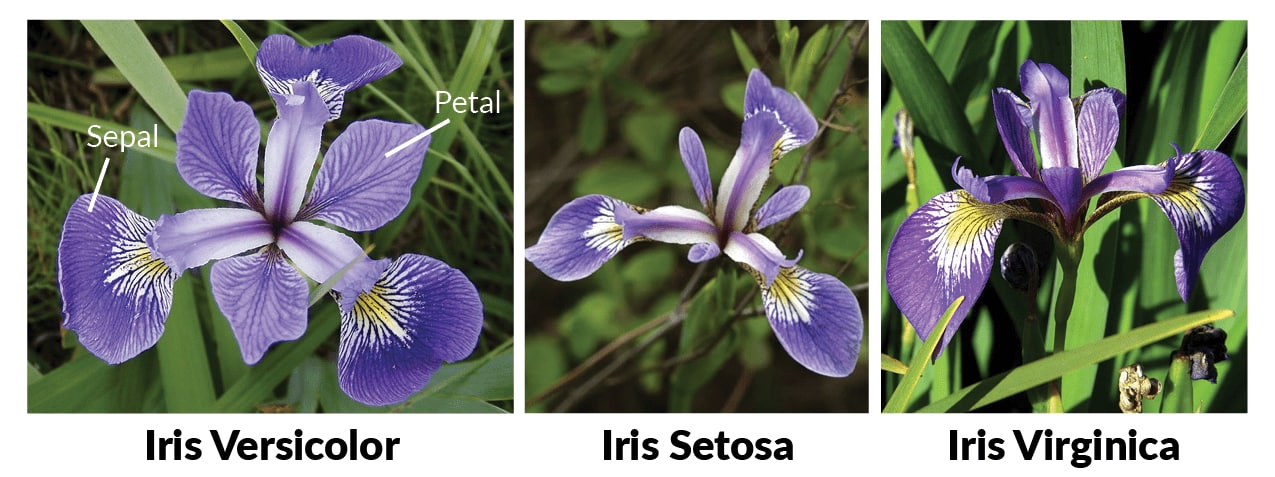
\includegraphics[width=0.85\linewidth]{plots/iris_picture}

Som vi også så i grundlæggende R, kan man indlæse et indbyggede datasæt med hjælp af funktionen \texttt{data()}.

\begin{Shaded}
\begin{Highlighting}[]
\FunctionTok{data}\NormalTok{(iris)}
\end{Highlighting}
\end{Shaded}

Først vil vi have et overblik over datasættet. Til at gøre dette bruger vi \texttt{summary()}:

\begin{Shaded}
\begin{Highlighting}[]
\FunctionTok{summary}\NormalTok{(iris)}
\end{Highlighting}
\end{Shaded}

\begin{verbatim}
##   Sepal.Length    Sepal.Width     Petal.Length    Petal.Width   
##  Min.   :4.300   Min.   :2.000   Min.   :1.000   Min.   :0.100  
##  1st Qu.:5.100   1st Qu.:2.800   1st Qu.:1.600   1st Qu.:0.300  
##  Median :5.800   Median :3.000   Median :4.350   Median :1.300  
##  Mean   :5.843   Mean   :3.057   Mean   :3.758   Mean   :1.199  
##  3rd Qu.:6.400   3rd Qu.:3.300   3rd Qu.:5.100   3rd Qu.:1.800  
##  Max.   :7.900   Max.   :4.400   Max.   :6.900   Max.   :2.500  
##        Species  
##  setosa    :50  
##  versicolor:50  
##  virginica :50  
##                 
##                 
## 
\end{verbatim}

Forestil, at vi gerne vil lave et plot, som viser sammenhængen mellem længden og bredden af sepal (bægerblad), eller specifikt er vi interesseret i kolonnerne \texttt{iris\$Sepal.Length} og \texttt{iris\$Sepal.Width}. Lad os starte med at visualisere variablerne i base-R, ved at bruge \texttt{plot}:

\begin{Shaded}
\begin{Highlighting}[]
\FunctionTok{plot}\NormalTok{(iris}\SpecialCharTok{$}\NormalTok{Sepal.Length, iris}\SpecialCharTok{$}\NormalTok{Sepal.Width)}
\end{Highlighting}
\end{Shaded}

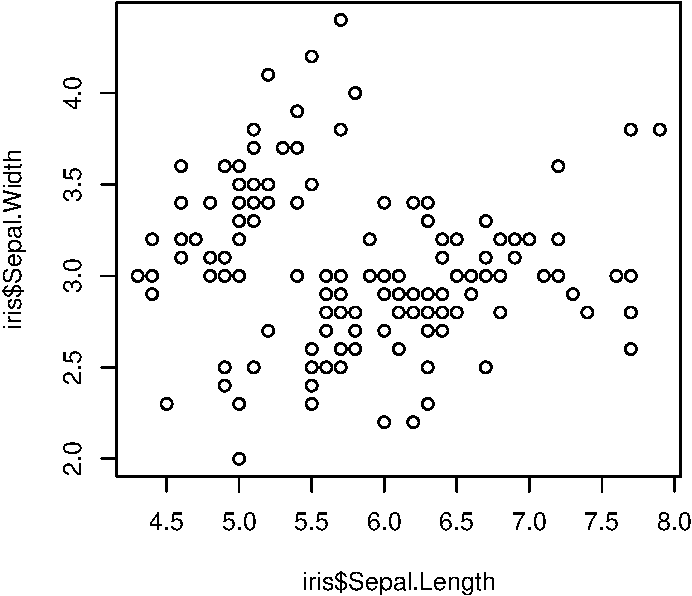
\includegraphics{visualisering_22_files/figure-latex/unnamed-chunk-116-1.pdf}

Man kan gøre det meget pænere eksempelvis ved at bruge forskellige farver til at betegne de forskellige arter, eller ved at give en hensigtsmæssig overskrift eller aksenavne.

\hypertarget{vores-fuxf8rste-ggplot}{%
\section{Vores første ggplot}\label{vores-fuxf8rste-ggplot}}

Vi vil imidlertid fokusere på at lave et lignende plot med pakken \texttt{ggplot2}. Hvis man ikke allerede har gjort det, så husk at indlæse pakken i R for at få nedenstående koder til at virke.

\begin{Shaded}
\begin{Highlighting}[]
\CommentTok{\#install.packages("ggplot2") \#hvis ikke allerede installeret}
\FunctionTok{library}\NormalTok{(ggplot2)}
\end{Highlighting}
\end{Shaded}

For at lave et plot med \texttt{ggplot2} tager man altid udgangspunkt i funktionen \texttt{ggplot()}. Først specificerer vi vores data - altså at vi gerne vil bruge dataframe \texttt{iris}. Dernæst angiver vi indenfor funktionen \texttt{aes()} (som sidder indenfor \texttt{ggplot()}), at x-aksen skal være \texttt{Sepal.Length} og y-aksen \texttt{Sepal.Width}. Det ser sådan ud:

\begin{Shaded}
\begin{Highlighting}[]
\FunctionTok{ggplot}\NormalTok{(iris, }\FunctionTok{aes}\NormalTok{(}\AttributeTok{x=}\NormalTok{Sepal.Length, }\AttributeTok{y=}\NormalTok{Sepal.Width))}
\end{Highlighting}
\end{Shaded}

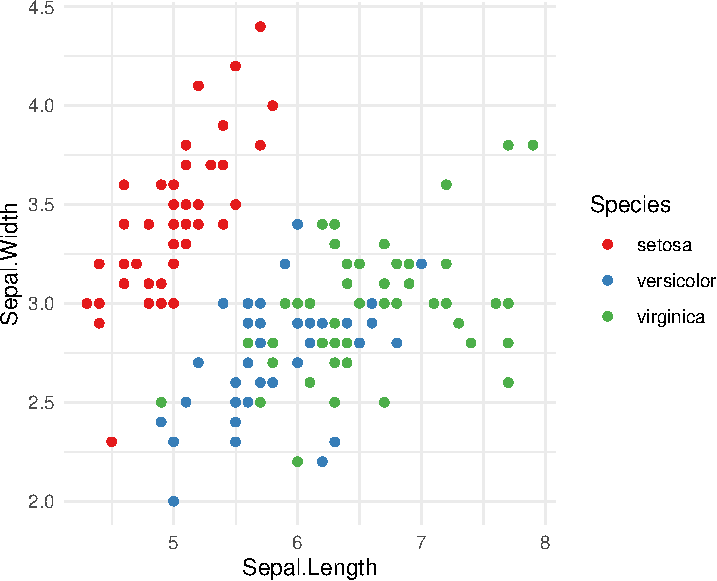
\includegraphics{visualisering_22_files/figure-latex/unnamed-chunk-118-1.pdf}

Koden fungerer, men bemærk at plottet er helt blank og derfor ikke særligt brugbart. Men der er blevet lavet et grundlag (se aksenavne osv.). Det er blank fordi vi endnu ikke har fortalt, hvilken plot type det skal være - for eksempel søljediagram/barplot, histogram, punktplot/scatter plot (jeg vælge de engelske begreber herfra for at skabe den bedste sammenhæng med koden). Vi vil gerne bruge et scatter plot, som i \textbf{ggplot2} er angivet af funktionen \texttt{geom\_point()}. Vi forbinder derfor funktionen \texttt{geom\_point()} til den \texttt{ggplot()} funktion, vi allerede har specificeret. Husk altid, at man bruger \texttt{+} til at forbinde de to ``komponenter'' (altså \texttt{ggplot()} og \texttt{geom\_point()}) af plottet (ellers få vi fortsat et blank plot).

Koden er således:

\begin{Shaded}
\begin{Highlighting}[]
\FunctionTok{ggplot}\NormalTok{(iris, }\FunctionTok{aes}\NormalTok{(}\AttributeTok{x=}\NormalTok{Sepal.Length, }\AttributeTok{y=}\NormalTok{Sepal.Width)) }\SpecialCharTok{+}
  \FunctionTok{geom\_point}\NormalTok{()}
\end{Highlighting}
\end{Shaded}

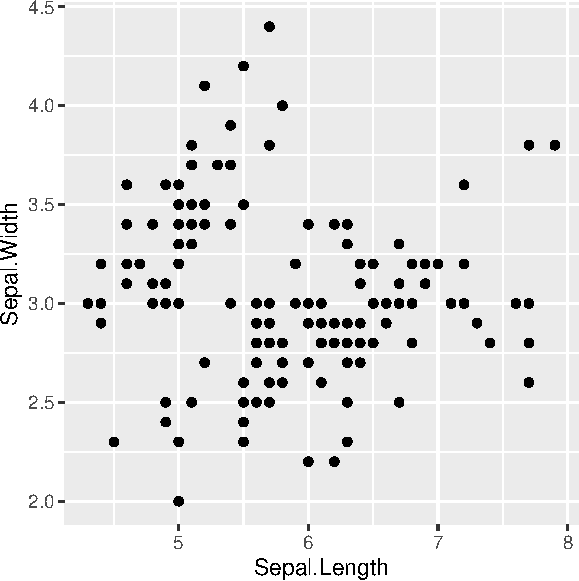
\includegraphics{visualisering_22_files/figure-latex/unnamed-chunk-119-1.pdf}

Bemærk, at vi ikke har skrevet noget indeni de runde parenteser i funktionen \texttt{geom\_point()}. Det betyder, at vi accepterer alle standard eller `default' parametre, som funktionen tager. Hvis vi vil have noget andet end de standard parametre, kan vi godt specificere det. For eksempel kan vi gøre punkterne lidt større end ved standard (prøve at tjekke \texttt{?geom\_point()} for at se en list overfor de mulige parametre, man kan justere på):

\begin{Shaded}
\begin{Highlighting}[]
\FunctionTok{ggplot}\NormalTok{(iris, }\FunctionTok{aes}\NormalTok{(}\AttributeTok{x=}\NormalTok{Sepal.Length, }\AttributeTok{y=}\NormalTok{Sepal.Width)) }\SpecialCharTok{+}
  \FunctionTok{geom\_point}\NormalTok{(}\AttributeTok{size=}\DecValTok{3}\NormalTok{)}
\end{Highlighting}
\end{Shaded}

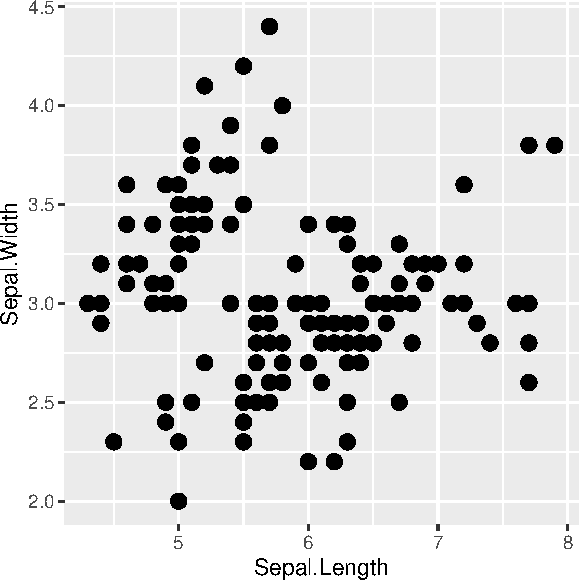
\includegraphics{visualisering_22_files/figure-latex/unnamed-chunk-120-1.pdf}

Vi har nu et plot, som vi kan sammenligne med det ovenstående plot, vi lavet i base-pakken. Ligesom i base-pakken vil vi gerne tilføje nogle ting for at gøre vores plot til vores \emph{færdige figur}.. Her i \textbf{ggplot2} gøres det ved at tilføje flere komponenter ovenpå, med brugen af \texttt{+}, ligesom vi gjorde da vi tilføjede \texttt{geom\_point()} til \texttt{ggplot()}. Første vil jeg gerne skrive nogle orde om \textbf{ggplot2} generelt, og filosofien bag.

\hypertarget{lidt-om-ggplot2}{%
\section{Lidt om ggplot2}\label{lidt-om-ggplot2}}

\hypertarget{syntax}{%
\subsection{Syntax}\label{syntax}}

Som vi har lige set, \texttt{ggplot()} tager altid udgangspunkt i en dataframe, som vi specificerer først. I \texttt{ggplot()} indeholder den dataframe variablerne vi skal bruge til at få lavet figuren. Til at gøre det til noget mere konkret, lad os sammenligne koden mellem base-pakken og \texttt{ggplot()} til vores \texttt{iris} data. I base-R angav vi direkte vektorer \texttt{iris\$Sepal.Length} og \texttt{iris\$Sepal.Width} som parametre \texttt{x} og \texttt{y}, der tager henholdsvis første og andens-plads i funktionen \texttt{plot()}. Til gengæld i \texttt{ggplot()}, specificerer man først den hele dataramme i den første plads, og så bagefter med brugen af \texttt{aes()} angav vi hvordan x-aksen og y-aksen ser ud.

\begin{Shaded}
\begin{Highlighting}[]
\CommentTok{\#baseplot solution}
\FunctionTok{plot}\NormalTok{(iris}\SpecialCharTok{$}\NormalTok{Sepal.Length, iris}\SpecialCharTok{$}\NormalTok{Sepal.Width) }

\CommentTok{\#ggplot2 solution}
\FunctionTok{ggplot}\NormalTok{(iris, }\FunctionTok{aes}\NormalTok{(}\AttributeTok{x=}\NormalTok{Sepal.Length, }\AttributeTok{y=}\NormalTok{Sepal.Width)) }\SpecialCharTok{+}
  \FunctionTok{geom\_point}\NormalTok{()}
\end{Highlighting}
\end{Shaded}

En anden fordel af \texttt{ggplot2()} er, at man kan blive ved med at forbedre plottet ved at tilføje ting ovenpå det plot, som vi allerede har lavet, i hvad man kan beskriver som en lagring tilgang. Det gøres intuitiv ved brugen af ``+''. Man kan derfor starte med noget simpelt, og derefter opbygge det til noget mere kompleks. Dette er uafhængig af den type plot, vi laver.

\hypertarget{hvad-betyder-egentlig-grammar-of-graphics}{%
\subsection{Hvad betyder egentlig grammar of graphics?}\label{hvad-betyder-egentlig-grammar-of-graphics}}

Den \texttt{gg} i \texttt{ggplot2} står for \emph{grammar of graphics}, og filosofien er at der skal defineres en \emph{sætningsstruktur} til de figurer, man laver. Med andre ord består vores figur af forskellige komponenter, som man forbinder med ``+''..

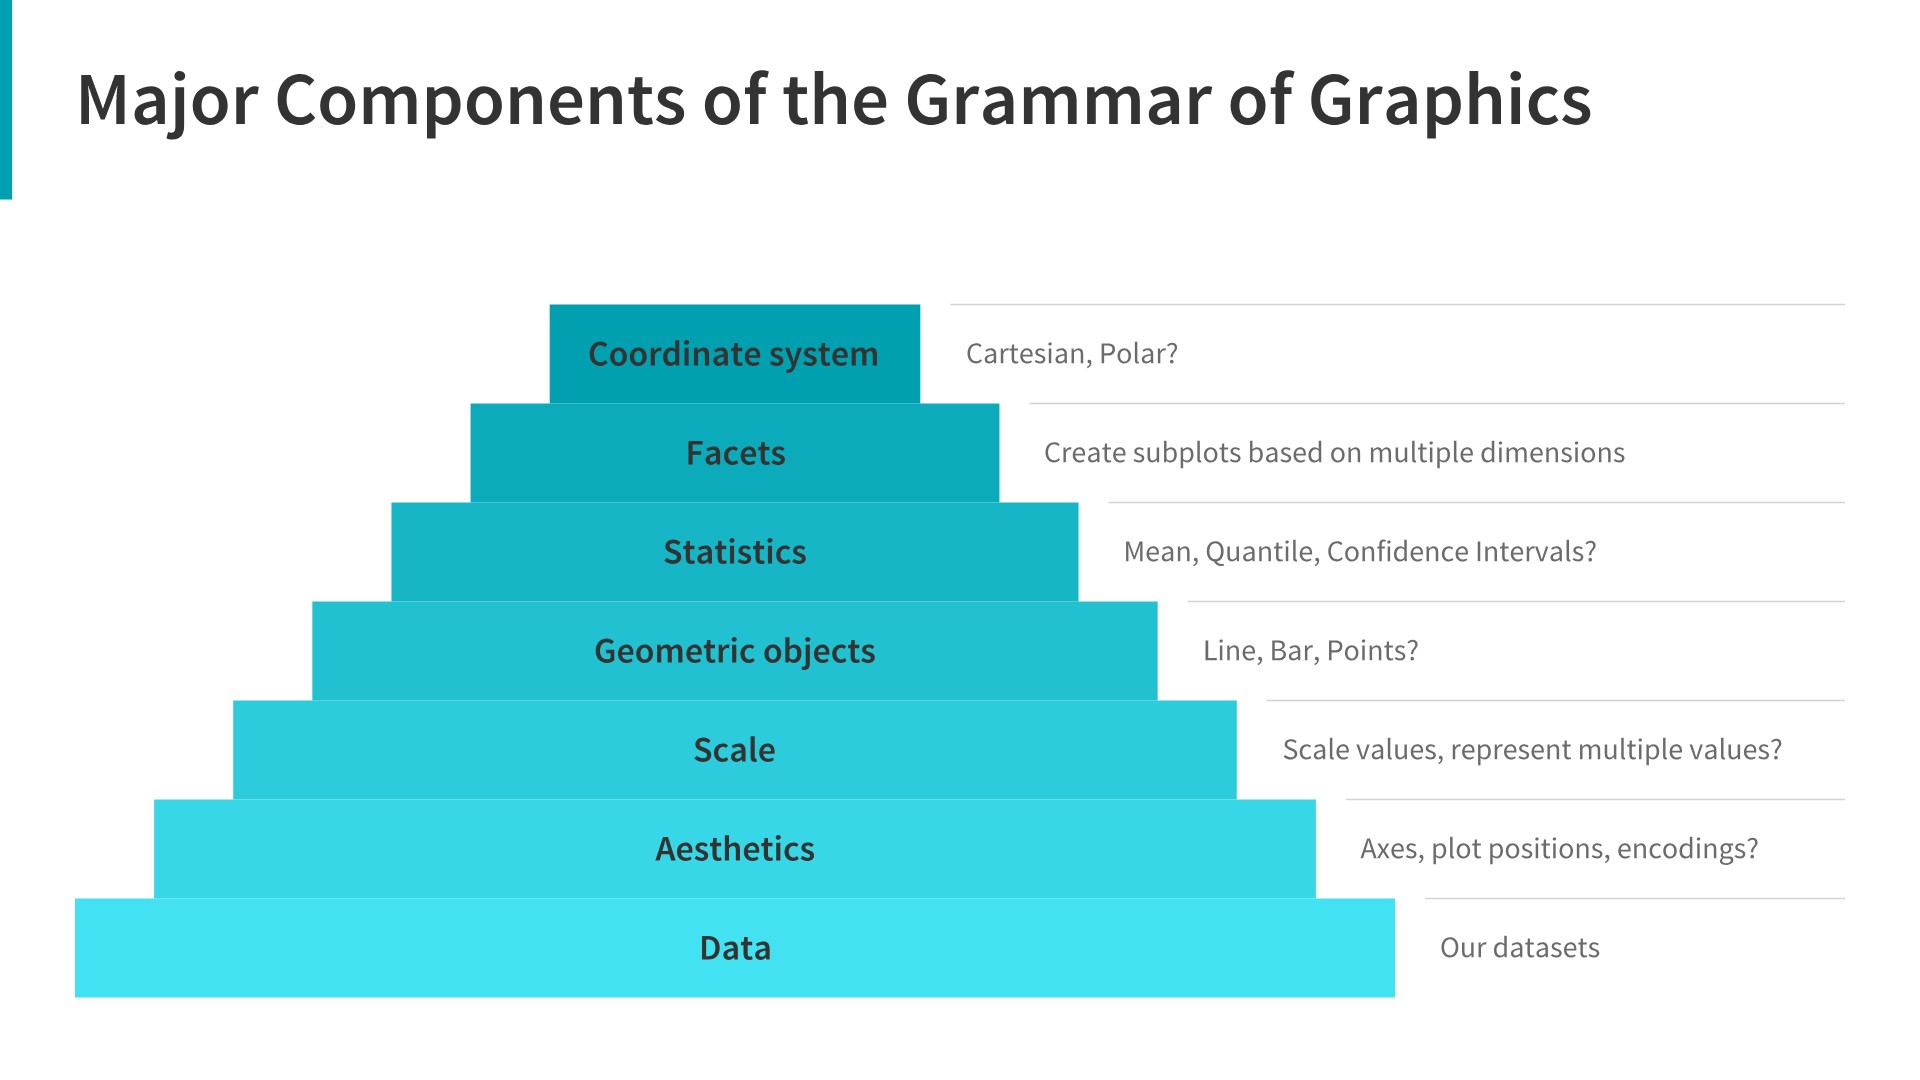
\includegraphics[width=0.5\linewidth]{plots/graphics_grammar}

Her er en beskrivelse af de forskellige komponenter til at opbygge et plot:

\begin{itemize}
\tightlist
\item
  Data: Datarammer tager altid udgangspunkt
\item
  Aesthetics: Variabler til x-aksen eller y-aksen, farve, form eller størrelse
\item
  Scale: Scalere værdier eller representere flere værdier
\item
  Geometries: Eller \texttt{geoms} - hvad type plot skal vi lave - fk. bars, points, lines osv.
\item
  Statistics: Tilføj fk. mean, median, quartile som beskrive data
\item
  Facets: Lave subplots baserende på flere dimensioner
\item
  Coordinate system: Transformerer akser, ændrer afstanden for de viste data
\end{itemize}

\hypertarget{globale-versus-lokale-uxe6stetik}{%
\subsection{Globale versus lokale æstetik}\label{globale-versus-lokale-uxe6stetik}}

De fleste tilfælde bruger vil funktionen \texttt{aes()} indenfor \texttt{ggplot()}, med betydningen, at variablerne specificeret indenfor \texttt{aes()} gælder globalt over alle komponenter i plottet. Man kan faktisk også skrive \texttt{aes()} lokale indenfor selve geom funktion, som i følgende:

\begin{Shaded}
\begin{Highlighting}[]
\FunctionTok{ggplot}\NormalTok{(iris) }\SpecialCharTok{+}
  \FunctionTok{geom\_point}\NormalTok{(}\FunctionTok{aes}\NormalTok{(}\AttributeTok{x=}\NormalTok{Sepal.Length, }\AttributeTok{y=}\NormalTok{Sepal.Width))}
\end{Highlighting}
\end{Shaded}

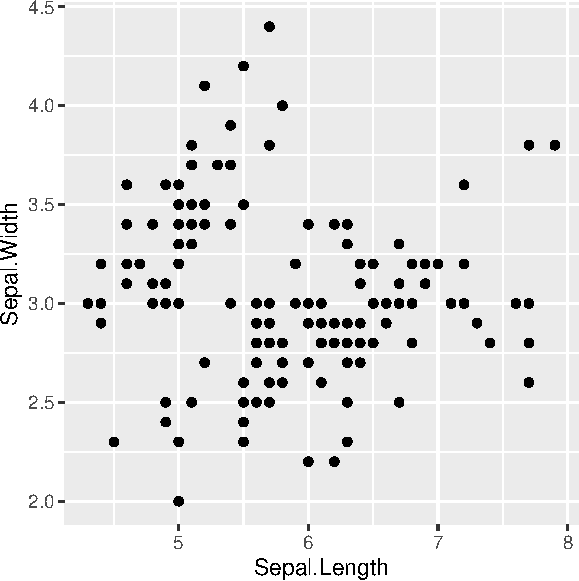
\includegraphics{visualisering_22_files/figure-latex/unnamed-chunk-123-1.pdf}

Vi får det samme plot som før, men det er kun \texttt{geom\_point()} der er påvirket af specificeringen indenfor \texttt{aes()}. I simpel situationer som ovenpå er der ingen forskel, men når man har mange forskellige komponenter i spil, så kan det nogle gange give mening at bruge lokale æstetik.

\hypertarget{specificere-etiketter-og-titel}{%
\section{Specificere etiketter og titel}\label{specificere-etiketter-og-titel}}

Vi tager udgangspunkt i plottet, vi lavet i ovenstående og prøver at gøre det bedre ved at tilføje nye etiketter og en titel. I \texttt{ggplot} kan man opdatere y-akse og x-akse etiketter ved at bruge henholdsvis \texttt{ylab} og \texttt{xlab}:

\begin{Shaded}
\begin{Highlighting}[]
\FunctionTok{ggplot}\NormalTok{(iris, }\FunctionTok{aes}\NormalTok{(}\AttributeTok{x=}\NormalTok{Sepal.Length, }\AttributeTok{y=}\NormalTok{Sepal.Width)) }\SpecialCharTok{+}
  \FunctionTok{geom\_point}\NormalTok{(}\AttributeTok{size=}\DecValTok{3}\NormalTok{) }\SpecialCharTok{+}
  \FunctionTok{xlab}\NormalTok{(}\StringTok{"Sepal Length"}\NormalTok{) }\SpecialCharTok{+}
  \FunctionTok{ylab}\NormalTok{(}\StringTok{"Sepal Width"}\NormalTok{)}
\end{Highlighting}
\end{Shaded}

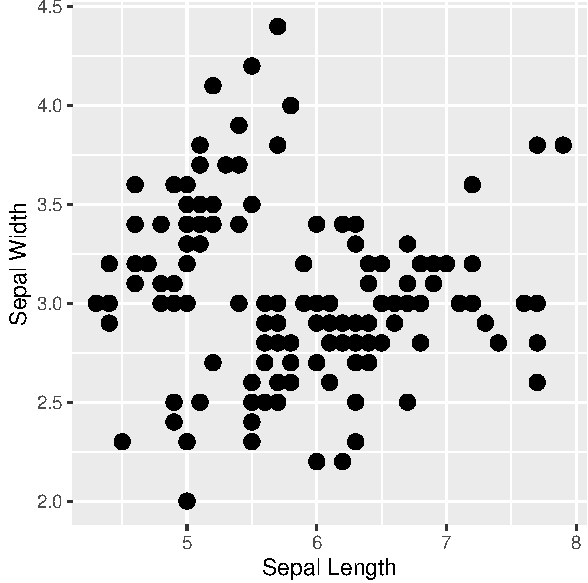
\includegraphics{visualisering_22_files/figure-latex/unnamed-chunk-124-1.pdf}

Vi tilføjer en titel med funktionen \texttt{ggtitle()}:

\begin{Shaded}
\begin{Highlighting}[]
\FunctionTok{ggplot}\NormalTok{(iris, }\FunctionTok{aes}\NormalTok{(}\AttributeTok{x=}\NormalTok{Sepal.Length, }\AttributeTok{y=}\NormalTok{Sepal.Width)) }\SpecialCharTok{+}
  \FunctionTok{geom\_point}\NormalTok{(}\AttributeTok{size=}\DecValTok{3}\NormalTok{) }\SpecialCharTok{+}
  \FunctionTok{xlab}\NormalTok{(}\StringTok{"Sepal Length"}\NormalTok{) }\SpecialCharTok{+}
  \FunctionTok{ylab}\NormalTok{(}\StringTok{"Sepal Width"}\NormalTok{) }\SpecialCharTok{+}
  \FunctionTok{ggtitle}\NormalTok{(}\StringTok{"Scatter plot of Sepal Width vs Sepal Length"}\NormalTok{)}
\end{Highlighting}
\end{Shaded}

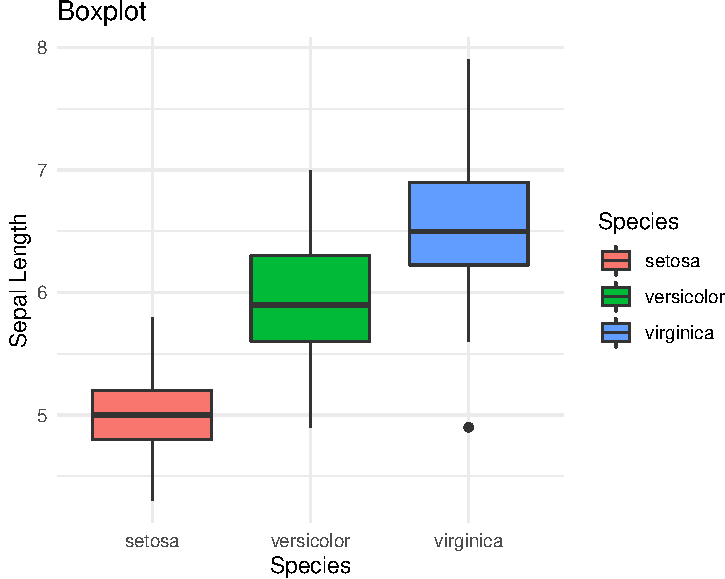
\includegraphics{visualisering_22_files/figure-latex/unnamed-chunk-125-1.pdf}

\hypertarget{uxe6ndre-farver}{%
\section{Ændre farver}\label{uxe6ndre-farver}}

I \texttt{ggplot2} kan man bruge ``automatisk'' farver for at skelne imellem de tre forskellige \texttt{Species} i datasættet \texttt{iris}. I næste lektion dækker jeg hvordan man kan være mere fleksibel ved at sætte farver manuelt, men ofte vil vi bare bruge som udgangspunkt den nemme løsning og eventuelle rette op på det bagefter med en ny komponent, hvis der er behov for det. Vi skriver \texttt{color=Species} indenfor \texttt{aes()}, som i følgende. Bemærk, at der kommer en `legend' med, der fortæller os, hvilken art få hvilken farve.

\begin{Shaded}
\begin{Highlighting}[]
\FunctionTok{ggplot}\NormalTok{(iris, }\FunctionTok{aes}\NormalTok{(}\AttributeTok{x=}\NormalTok{Sepal.Length, }\AttributeTok{y=}\NormalTok{Sepal.Width,}\AttributeTok{color=}\NormalTok{Species)) }\SpecialCharTok{+}
  \FunctionTok{geom\_point}\NormalTok{(}\AttributeTok{size=}\DecValTok{3}\NormalTok{) }\SpecialCharTok{+}
  \FunctionTok{xlab}\NormalTok{(}\StringTok{"Sepal Length"}\NormalTok{) }\SpecialCharTok{+}
  \FunctionTok{ylab}\NormalTok{(}\StringTok{"Sepal Width"}\NormalTok{) }\SpecialCharTok{+}
  \FunctionTok{ggtitle}\NormalTok{(}\StringTok{"Scatter plot of Sepal Width vs Sepal Length"}\NormalTok{)}
\end{Highlighting}
\end{Shaded}

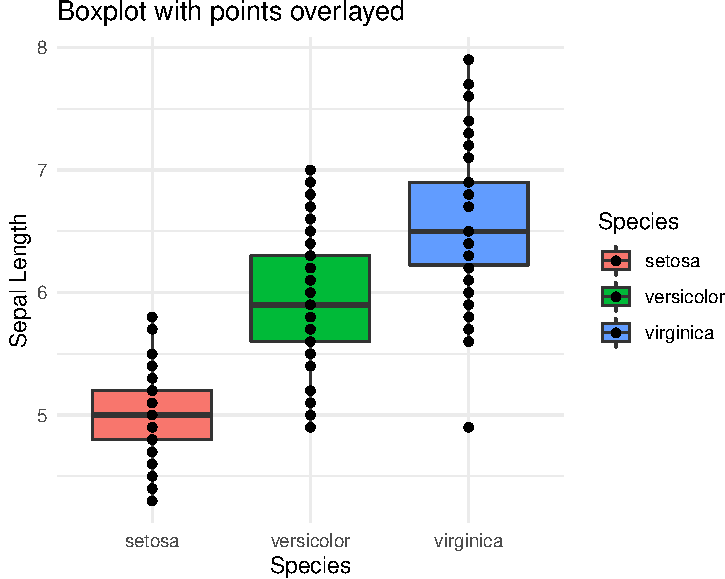
\includegraphics{visualisering_22_files/figure-latex/unnamed-chunk-126-1.pdf}

\hypertarget{uxe6ndre-tema}{%
\section{Ændre tema}\label{uxe6ndre-tema}}

Det standard tema har en grå baggrund og ``grid'' linjer, men vi kan godt vælge noget andet. For eksempel kan man tilføje \texttt{theme\_minimal()} som i nedenstående. Her får vi en hvid baggrund i stedet for, mens vi får stadig grid linjer. Man kan afprøve forskellige temaer (for eksempel \texttt{theme\_classic()}, \texttt{theme\_bw()}), og se, hvilket tema fungerer bedst i det enkelt plot.

\begin{Shaded}
\begin{Highlighting}[]
\FunctionTok{ggplot}\NormalTok{(iris, }\FunctionTok{aes}\NormalTok{(}\AttributeTok{x=}\NormalTok{Sepal.Length, }\AttributeTok{y=}\NormalTok{Sepal.Width,}\AttributeTok{color=}\NormalTok{Species)) }\SpecialCharTok{+}
  \FunctionTok{geom\_point}\NormalTok{(}\AttributeTok{size=}\DecValTok{3}\NormalTok{) }\SpecialCharTok{+}
  \FunctionTok{xlab}\NormalTok{(}\StringTok{"Sepal Length"}\NormalTok{) }\SpecialCharTok{+}
  \FunctionTok{ylab}\NormalTok{(}\StringTok{"Sepal Width"}\NormalTok{) }\SpecialCharTok{+}
  \FunctionTok{ggtitle}\NormalTok{(}\StringTok{"Scatter plot of Sepal Width vs Sepal Length"}\NormalTok{) }\SpecialCharTok{+}
  \FunctionTok{theme\_minimal}\NormalTok{()}
\end{Highlighting}
\end{Shaded}

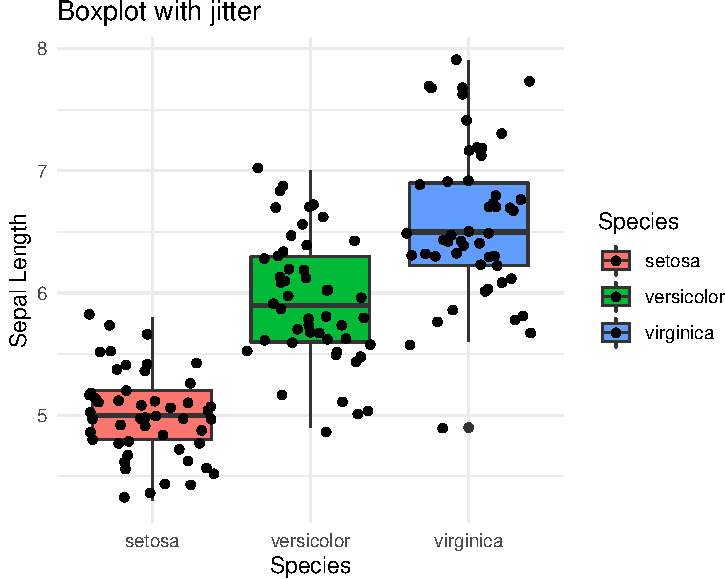
\includegraphics{visualisering_22_files/figure-latex/unnamed-chunk-127-1.pdf}

Her er nogle eksempler på mulige temaer du kan bruge i dine plotter (det er dog generelt op til dig).

\begin{longtable}[]{@{}l@{}}
\toprule
tema \\
\midrule
\endhead
\texttt{theme\_grey()} \\
\texttt{theme\_classic()} \\
\texttt{theme\_bw()} \\
\texttt{theme\_dark()} \\
\texttt{theme\_minimal()} \\
\texttt{theme\_light()} \\
\bottomrule
\end{longtable}

Se også her hvis du er interesseret i flere temaer: \url{https://r-charts.com/ggplot2/themes/}

\hypertarget{forskellige-geoms}{%
\section{Forskellige geoms}\label{forskellige-geoms}}

Indtil videre har vi kun arbejdet med \texttt{geom\_point()} for at lave et scatter plot, men det kan være at vi gerne vil lave noget andet. Her gennemgår jeg følgende ``geoms'':

\begin{longtable}[]{@{}ll@{}}
\toprule
geom & plot \\
\midrule
\endhead
\texttt{geom\_point()} & scatter plot \\
\texttt{geom\_bar()} & barplot \\
\texttt{geom\_boxplot()} & boxplot \\
\texttt{geom\_histogram()} & histogram \\
\texttt{geom\_density()} & density \\
\bottomrule
\end{longtable}

For at lave disse geoms, skal man tillægge funktionen til den \texttt{ggplot()} kommando med \texttt{+}, ligesom vi gjorde med \texttt{geom\_point()}. Der kan dog være for nogle plot-typer specifikke overvejelser, som er værd at vide inden man selv bruger dem.

\hypertarget{boxplot-geom_box}{%
\subsection{\texorpdfstring{Boxplot (\texttt{geom\_box})}{Boxplot (geom\_box)}}\label{boxplot-geom_box}}

For at lave et boxplot af \texttt{Sepal.Length} opdelt efter \texttt{Species}, angiver vi \texttt{Species} på x-aksen og \texttt{Sepal.Length} på y-aksen. Vi vil også have, at hver art få sin egen farve, så bruger vi \texttt{fill=Species}.

\begin{Shaded}
\begin{Highlighting}[]
\FunctionTok{ggplot}\NormalTok{(}\AttributeTok{data=}\NormalTok{iris, }\FunctionTok{aes}\NormalTok{(}\AttributeTok{x=}\NormalTok{Species, }\AttributeTok{y=}\NormalTok{Sepal.Length,}\AttributeTok{fill=}\NormalTok{Species)) }\SpecialCharTok{+} 
  \FunctionTok{geom\_boxplot}\NormalTok{() }\SpecialCharTok{+} 
  \FunctionTok{ylab}\NormalTok{(}\StringTok{"Sepal Length"}\NormalTok{) }\SpecialCharTok{+} 
  \FunctionTok{ggtitle}\NormalTok{(}\StringTok{"Boxplot"}\NormalTok{) }\SpecialCharTok{+}
  \FunctionTok{theme\_minimal}\NormalTok{()}
\end{Highlighting}
\end{Shaded}

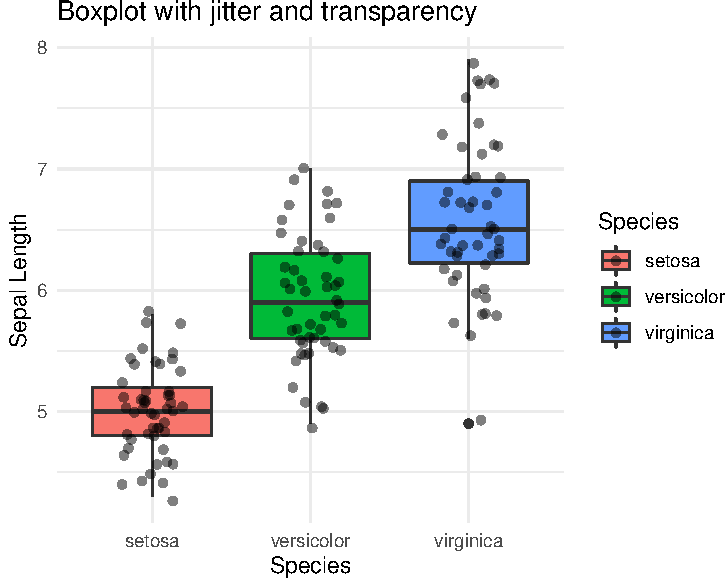
\includegraphics{visualisering_22_files/figure-latex/unnamed-chunk-128-1.pdf}

\textbf{Lave punkter ovenpå}

Det kan ofte være nyttigt at plotte de egentlige data punkter ovenpå boxplottet, så I kan se både fordelingen i de data samt de rå data. En løsning er at benytte \texttt{geom\_point()} ved at tilføje det som komponent over vores eksisterende kode.

\begin{Shaded}
\begin{Highlighting}[]
\FunctionTok{ggplot}\NormalTok{(}\AttributeTok{data=}\NormalTok{iris, }\FunctionTok{aes}\NormalTok{(}\AttributeTok{x=}\NormalTok{Species, }\AttributeTok{y=}\NormalTok{Sepal.Length,}\AttributeTok{fill=}\NormalTok{Species)) }\SpecialCharTok{+} 
  \FunctionTok{geom\_boxplot}\NormalTok{() }\SpecialCharTok{+} 
  \FunctionTok{geom\_point}\NormalTok{() }\SpecialCharTok{+} 
  \FunctionTok{ylab}\NormalTok{(}\StringTok{"Sepal Length"}\NormalTok{) }\SpecialCharTok{+} 
  \FunctionTok{ggtitle}\NormalTok{(}\StringTok{"Boxplot with points overlayed"}\NormalTok{) }\SpecialCharTok{+} 
  \FunctionTok{theme\_minimal}\NormalTok{()}
\end{Highlighting}
\end{Shaded}

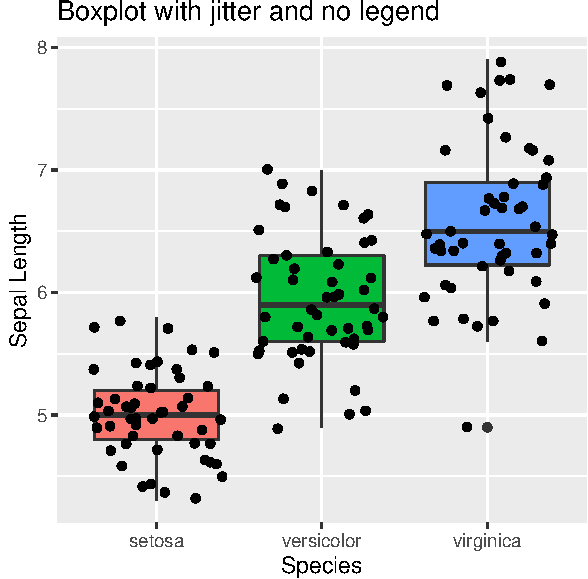
\includegraphics{visualisering_22_files/figure-latex/unnamed-chunk-129-1.pdf}

Man kan dog se, at det ikke er særlig informativ, da alle punkter er på den samme lodrette linje. Hvis vi har mange punkter med samme eller næsten samme værdier, så kan vi ikke se de fleste af dem i plottet. En bedre løsning er at indføre noget tilfældighed i punkterne langt x-aksen, så at man mere tydelige kan se dem. Det er kaldes for ``jitter'' og man specificerer jitter ved at bruge \texttt{geom\_jitter} i stedet for \texttt{geom\_point}.

\begin{Shaded}
\begin{Highlighting}[]
\FunctionTok{ggplot}\NormalTok{(}\AttributeTok{data=}\NormalTok{iris, }\FunctionTok{aes}\NormalTok{(}\AttributeTok{x=}\NormalTok{Species, }\AttributeTok{y=}\NormalTok{Sepal.Length,}\AttributeTok{fill=}\NormalTok{Species)) }\SpecialCharTok{+} 
  \FunctionTok{geom\_boxplot}\NormalTok{() }\SpecialCharTok{+} 
  \FunctionTok{geom\_jitter}\NormalTok{() }\SpecialCharTok{+}
  \FunctionTok{ylab}\NormalTok{(}\StringTok{"Sepal Length"}\NormalTok{) }\SpecialCharTok{+} 
  \FunctionTok{ggtitle}\NormalTok{(}\StringTok{"Boxplot with jitter"}\NormalTok{) }\SpecialCharTok{+} 
  \FunctionTok{theme\_minimal}\NormalTok{()}
\end{Highlighting}
\end{Shaded}

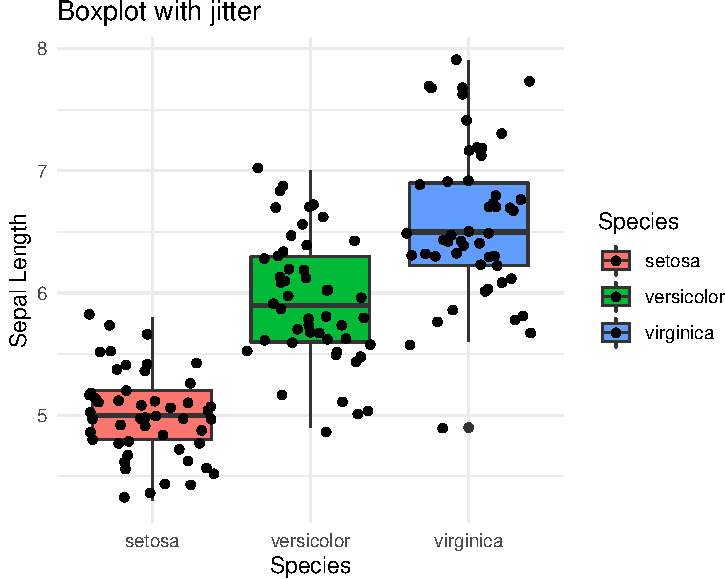
\includegraphics{visualisering_22_files/figure-latex/unnamed-chunk-130-1.pdf}

Jeg kan vi også specificere \texttt{alpha}, som indføre gøre punkterne gennemsigtige, for at gøre dem mindre markant. Man kan også ændre på \texttt{width} som kontrollerer deres spredning langt x-axsen.

\begin{Shaded}
\begin{Highlighting}[]
\FunctionTok{ggplot}\NormalTok{(}\AttributeTok{data=}\NormalTok{iris, }\FunctionTok{aes}\NormalTok{(}\AttributeTok{x=}\NormalTok{Species, }\AttributeTok{y=}\NormalTok{Sepal.Length,}\AttributeTok{fill=}\NormalTok{Species)) }\SpecialCharTok{+} 
  \FunctionTok{geom\_boxplot}\NormalTok{() }\SpecialCharTok{+} 
  \FunctionTok{geom\_jitter}\NormalTok{(}\AttributeTok{alpha=}\FloatTok{0.5}\NormalTok{,}\AttributeTok{width=}\FloatTok{0.2}\NormalTok{) }\SpecialCharTok{+}
  \FunctionTok{ylab}\NormalTok{(}\StringTok{"Sepal Length"}\NormalTok{) }\SpecialCharTok{+} 
  \FunctionTok{ggtitle}\NormalTok{(}\StringTok{"Boxplot with jitter and transparency"}\NormalTok{) }\SpecialCharTok{+} 
  \FunctionTok{theme\_minimal}\NormalTok{()}
\end{Highlighting}
\end{Shaded}

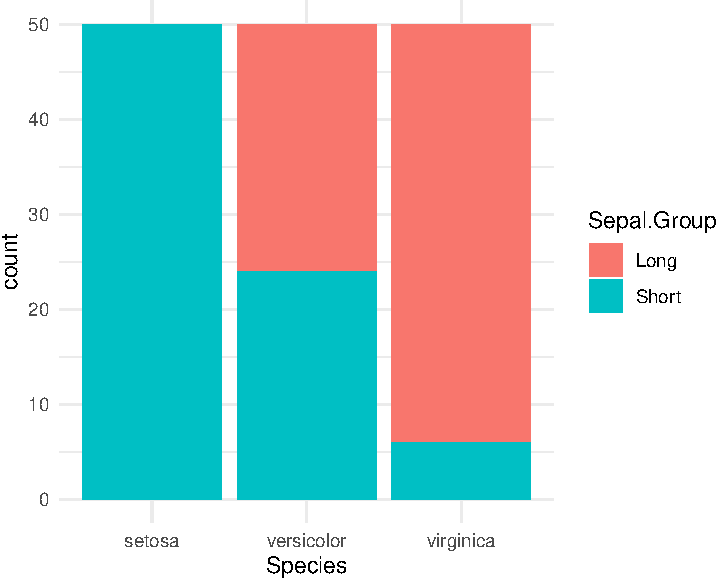
\includegraphics{visualisering_22_files/figure-latex/unnamed-chunk-131-1.pdf}

\textbf{Fjerne legend hvis unødvendige}

Man kan se, at når man specificerer farver, få man en legend på højre side af plotte. I dette tilfælde er det faktisk ikke nødvendige, da man kan se uden legend hvad de tre boxplots refererer til. Defor fjerner vi den fra plottet ved at bruge \texttt{theme(legend.position="none")}.

\begin{Shaded}
\begin{Highlighting}[]
\FunctionTok{ggplot}\NormalTok{(}\AttributeTok{data=}\NormalTok{iris, }\FunctionTok{aes}\NormalTok{(}\AttributeTok{x=}\NormalTok{Species, }\AttributeTok{y=}\NormalTok{Sepal.Length,}\AttributeTok{fill=}\NormalTok{Species)) }\SpecialCharTok{+} 
  \FunctionTok{geom\_boxplot}\NormalTok{() }\SpecialCharTok{+} 
  \FunctionTok{geom\_jitter}\NormalTok{() }\SpecialCharTok{+}
  \FunctionTok{ylab}\NormalTok{(}\StringTok{"Sepal Length"}\NormalTok{) }\SpecialCharTok{+} 
  \FunctionTok{ggtitle}\NormalTok{(}\StringTok{"Boxplot with jitter and no legend"}\NormalTok{) }\SpecialCharTok{+}
  \FunctionTok{theme}\NormalTok{(}\AttributeTok{legend.position=}\StringTok{"none"}\NormalTok{)}
\end{Highlighting}
\end{Shaded}

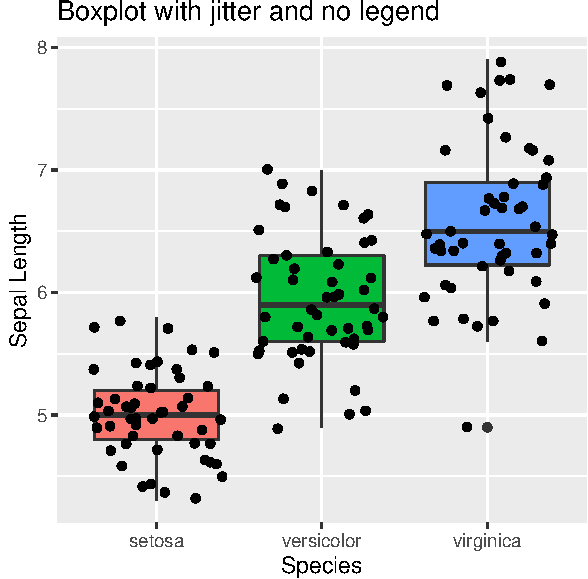
\includegraphics{visualisering_22_files/figure-latex/unnamed-chunk-132-1.pdf}

\hypertarget{barplot-geom_bar}{%
\subsection{\texorpdfstring{Barplot (\texttt{geom\_bar})}{Barplot (geom\_bar)}}\label{barplot-geom_bar}}

Med \texttt{ggplot()} kan man representere data i et bar plot ved at bruge \texttt{geom\_bar()}. I følgende vil vi gerne tælle op de antal observationer for hver art (variable \texttt{Species}), og visualiser dem således som søjler. Indenfor \texttt{geom\_bar()} specificerer vi således \texttt{stat="count"}.

Vi bruger også \texttt{fill=Species} her for at lave en forskellige farve automatiske for hver af de tre arter. Bemærk, at det var \texttt{color=Species} i det forudgående plot når vi anvendte \texttt{geom\_point()}. Det er fordi, \texttt{color} bruges for punkter og linjer, mens \texttt{fill} er til større regioner bliver udfyldt, såsom bars og histograms.

\begin{Shaded}
\begin{Highlighting}[]
\FunctionTok{ggplot}\NormalTok{(iris, }\FunctionTok{aes}\NormalTok{(}\AttributeTok{x=}\NormalTok{Species,}\AttributeTok{fill=}\NormalTok{Species)) }\SpecialCharTok{+} 
  \FunctionTok{geom\_bar}\NormalTok{(}\AttributeTok{stat =} \StringTok{"count"}\NormalTok{) }\SpecialCharTok{+}
  \FunctionTok{ggtitle}\NormalTok{(}\StringTok{"Number of observations by species"}\NormalTok{) }\SpecialCharTok{+}
  \FunctionTok{theme\_minimal}\NormalTok{()}
\end{Highlighting}
\end{Shaded}

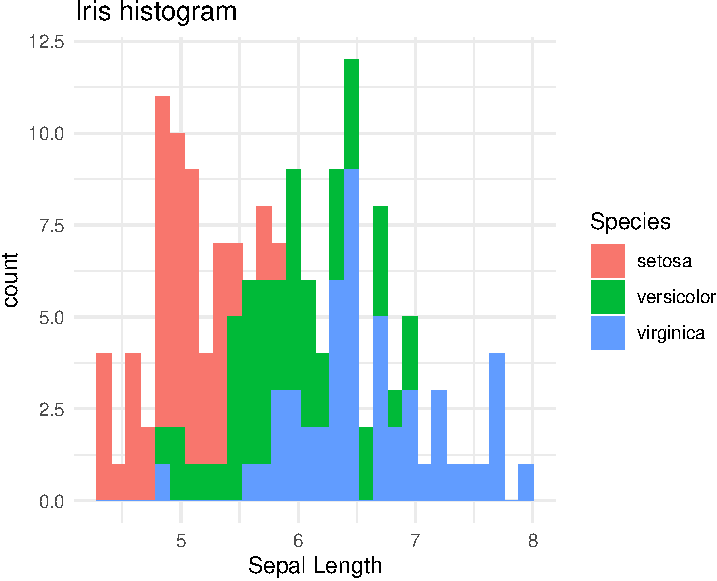
\includegraphics{visualisering_22_files/figure-latex/unnamed-chunk-133-1.pdf}

\textbf{Barplot: stack vs dodge}

Hvis man har flere katagoriske variabler, kan man lave barplots på forskellige måder. Da der er en ekstra katagorisk variabel i datasættet, laver jeg én, der hedder \texttt{Sepal.Group}, der skelne imellem \texttt{Long} og \texttt{Short} værdier af variablen \texttt{Sepal.Length}. Her specificerer jeg bare (med funktionen \texttt{ifelse()}), at hvis \texttt{Sepal.Length} er længere end den gennemsnitlige \texttt{Sepal.Length}, så er det betragtet \texttt{Long}, ellers er det \texttt{Short}, som i følgende:

\begin{Shaded}
\begin{Highlighting}[]
\NormalTok{iris}\SpecialCharTok{$}\NormalTok{Sepal.Group }\OtherTok{\textless{}{-}} 
  \FunctionTok{ifelse}\NormalTok{(iris}\SpecialCharTok{$}\NormalTok{Sepal.Length}\SpecialCharTok{\textgreater{}}\FunctionTok{mean}\NormalTok{(iris}\SpecialCharTok{$}\NormalTok{Sepal.Length),  }\CommentTok{\#test}
         \StringTok{"Long"}\NormalTok{,                                     }\CommentTok{\#if TRUE}
         \StringTok{"Short"}\NormalTok{)                                    }\CommentTok{\#if FALSE}
\end{Highlighting}
\end{Shaded}

Når jeg laver en barplot med de to variabler, tilføjer jeg \texttt{Sepal.Group} med \texttt{fill}, og \texttt{ggplot} splitter antal observationer efter \texttt{Sepal.Group} med farver som repræsenterer \texttt{Sepal.Group}, og tilføjer en tilsvarende legend.

\begin{Shaded}
\begin{Highlighting}[]
\FunctionTok{ggplot}\NormalTok{(iris, }\FunctionTok{aes}\NormalTok{(}\AttributeTok{x=}\NormalTok{Species, }\AttributeTok{fill=}\NormalTok{Sepal.Group)) }\SpecialCharTok{+} 
  \FunctionTok{geom\_bar}\NormalTok{(}\AttributeTok{stat =} \StringTok{"count"}\NormalTok{) }\SpecialCharTok{+}
  \FunctionTok{ggtitle}\NormalTok{(}\StringTok{"Number of observations by species"}\NormalTok{) }\SpecialCharTok{+}
  \FunctionTok{theme\_minimal}\NormalTok{()}
\end{Highlighting}
\end{Shaded}

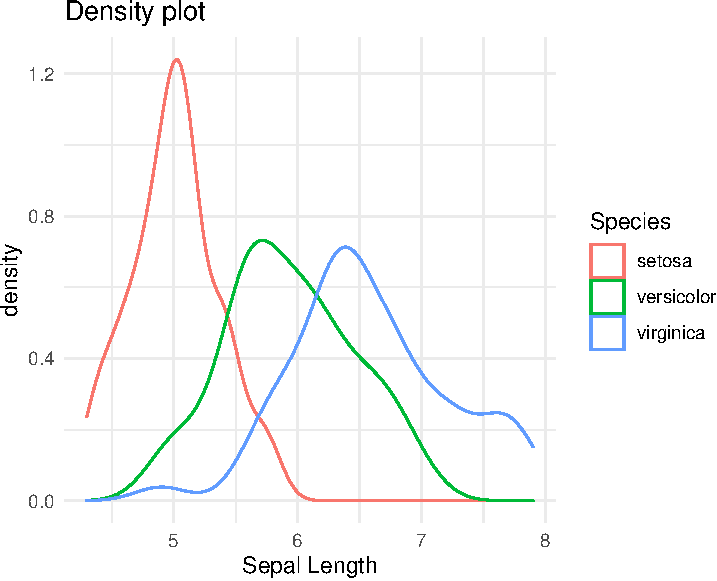
\includegraphics{visualisering_22_files/figure-latex/unnamed-chunk-135-1.pdf}

Mange gange foretrækker man at få bars som stå ved siden af hinanden. Det kan vi specificere med blot at tilføje \texttt{position="dodge"} ind i \texttt{geom\_bar()}.

\begin{Shaded}
\begin{Highlighting}[]
\FunctionTok{ggplot}\NormalTok{(iris, }\FunctionTok{aes}\NormalTok{(}\AttributeTok{x=}\NormalTok{Species, }\AttributeTok{fill=}\NormalTok{Sepal.Group)) }\SpecialCharTok{+} 
  \FunctionTok{geom\_bar}\NormalTok{(}\AttributeTok{stat =} \StringTok{"count"}\NormalTok{, }\AttributeTok{position =} \StringTok{"dodge"}\NormalTok{) }\SpecialCharTok{+}
  \FunctionTok{ggtitle}\NormalTok{(}\StringTok{"Number of observations by species"}\NormalTok{) }\SpecialCharTok{+}
  \FunctionTok{theme\_minimal}\NormalTok{()}
\end{Highlighting}
\end{Shaded}

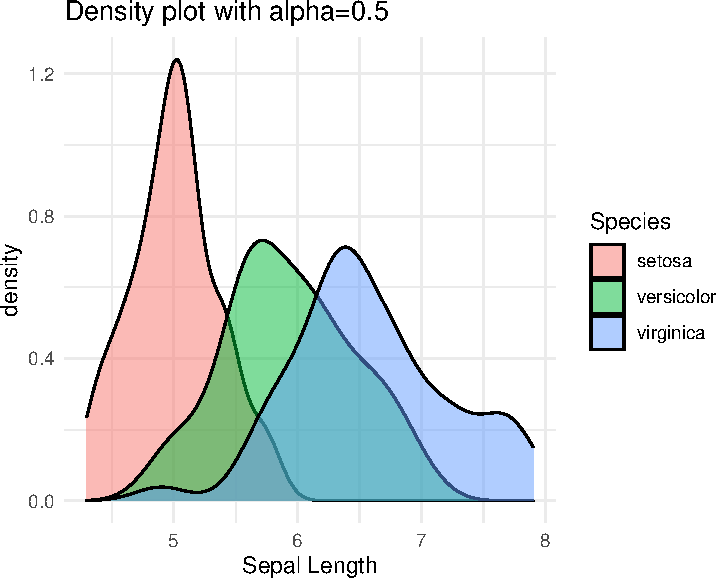
\includegraphics{visualisering_22_files/figure-latex/unnamed-chunk-136-1.pdf}

Som ekstra for at vise fleksibiliten i pakken \texttt{ggplot2}: jeg kan ikke lide at bredden af søjlen til arten setosa i ovenstående plot har bredden som er to gange større end de andre søjler (fordi der er ingen observationer i setosa som har ``Long'' i variablen \texttt{Sepal.Group}). Jeg Gogglede mig frem til en løsning på det:

\begin{Shaded}
\begin{Highlighting}[]
\FunctionTok{ggplot}\NormalTok{(iris, }\FunctionTok{aes}\NormalTok{(}\AttributeTok{x=}\NormalTok{Species, }\AttributeTok{fill=}\NormalTok{Sepal.Group)) }\SpecialCharTok{+} 
  \FunctionTok{geom\_bar}\NormalTok{(}\AttributeTok{stat =} \StringTok{"count"}\NormalTok{, }\AttributeTok{position =} \FunctionTok{position\_dodge2}\NormalTok{(}\AttributeTok{preserve =} \StringTok{"single"}\NormalTok{)) }\SpecialCharTok{+}
  \FunctionTok{ggtitle}\NormalTok{(}\StringTok{"Number of observations by species"}\NormalTok{) }\SpecialCharTok{+}
  \FunctionTok{theme\_minimal}\NormalTok{()}
\end{Highlighting}
\end{Shaded}

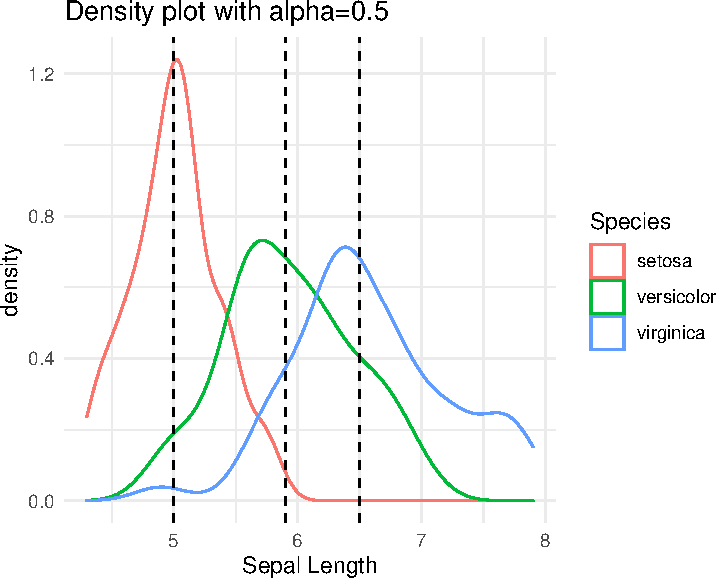
\includegraphics{visualisering_22_files/figure-latex/unnamed-chunk-137-1.pdf}

\hypertarget{histogram-geom_histogram}{%
\subsection{\texorpdfstring{Histogram (\texttt{geom\_histogram})}{Histogram (geom\_histogram)}}\label{histogram-geom_histogram}}

En histogram bruges til at få overblik over hvordan data fordeler sig. I \texttt{ggplot2} kan man lave en histogram med \texttt{geom\_histogram()}. Den x-akse variabel skal være en `continuous' variabel. Her specificerer vi, at vi gerne vil have et histogram for hver Species.

\begin{Shaded}
\begin{Highlighting}[]
\FunctionTok{ggplot}\NormalTok{(}\AttributeTok{data=}\NormalTok{iris, }\FunctionTok{aes}\NormalTok{(}\AttributeTok{x=}\NormalTok{Sepal.Length, }\AttributeTok{fill=}\NormalTok{Species)) }\SpecialCharTok{+} 
  \FunctionTok{geom\_histogram}\NormalTok{() }\SpecialCharTok{+} 
  \FunctionTok{xlab}\NormalTok{(}\StringTok{"Sepal Length"}\NormalTok{) }\SpecialCharTok{+} 
  \FunctionTok{ggtitle}\NormalTok{(}\StringTok{"Iris histogram"}\NormalTok{) }\SpecialCharTok{+} 
  \FunctionTok{theme\_minimal}\NormalTok{()}
\end{Highlighting}
\end{Shaded}

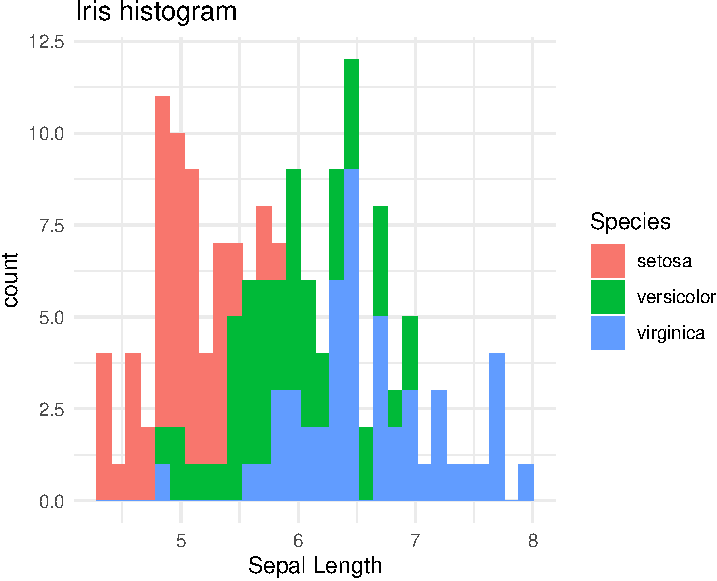
\includegraphics{visualisering_22_files/figure-latex/unnamed-chunk-138-1.pdf}

Man kan også gøre det nemmere at skelne imellem de tre arter ved at sætte \texttt{alpha=0.5} indenfor \texttt{geom\_histogram} og ved at angive en linje farve som mulighed inden for \texttt{geom\_histogram()}.

\begin{Shaded}
\begin{Highlighting}[]
\FunctionTok{ggplot}\NormalTok{(}\AttributeTok{data=}\NormalTok{iris, }\FunctionTok{aes}\NormalTok{(}\AttributeTok{x=}\NormalTok{Sepal.Length, }\AttributeTok{fill=}\NormalTok{Species)) }\SpecialCharTok{+} 
  \FunctionTok{geom\_histogram}\NormalTok{(}\AttributeTok{alpha=}\FloatTok{0.5}\NormalTok{,}\AttributeTok{color=}\StringTok{"black"}\NormalTok{) }\SpecialCharTok{+} 
  \FunctionTok{xlab}\NormalTok{(}\StringTok{"Sepal Length"}\NormalTok{) }\SpecialCharTok{+} 
  \FunctionTok{ggtitle}\NormalTok{(}\StringTok{"Iris histogram"}\NormalTok{) }\SpecialCharTok{+} 
  \FunctionTok{theme\_minimal}\NormalTok{()}
\end{Highlighting}
\end{Shaded}

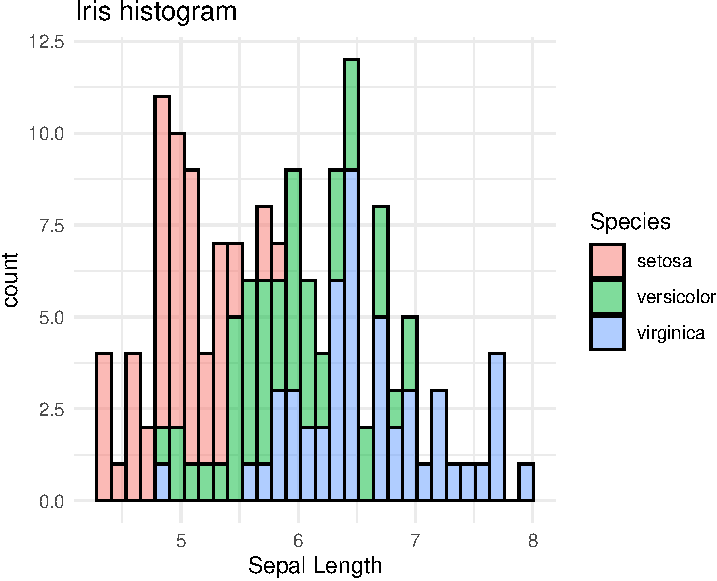
\includegraphics{visualisering_22_files/figure-latex/unnamed-chunk-139-1.pdf}

\hypertarget{density-geom_density}{%
\subsection{\texorpdfstring{Density (\texttt{geom\_density})}{Density (geom\_density)}}\label{density-geom_density}}

Med en density plot, ligesom med en histogram, kan man se fordelingen, de data har, i formen af en glat (eller ``smooth'') kurv.

\begin{Shaded}
\begin{Highlighting}[]
\FunctionTok{ggplot}\NormalTok{(}\AttributeTok{data=}\NormalTok{iris, }\FunctionTok{aes}\NormalTok{(}\AttributeTok{x=}\NormalTok{Sepal.Length, }\AttributeTok{color=}\NormalTok{Species)) }\SpecialCharTok{+} 
  \FunctionTok{geom\_density}\NormalTok{() }\SpecialCharTok{+} 
  \FunctionTok{xlab}\NormalTok{(}\StringTok{"Sepal Length"}\NormalTok{) }\SpecialCharTok{+} 
  \FunctionTok{ggtitle}\NormalTok{(}\StringTok{"Density plot"}\NormalTok{) }\SpecialCharTok{+}
  \FunctionTok{theme\_minimal}\NormalTok{()}
\end{Highlighting}
\end{Shaded}

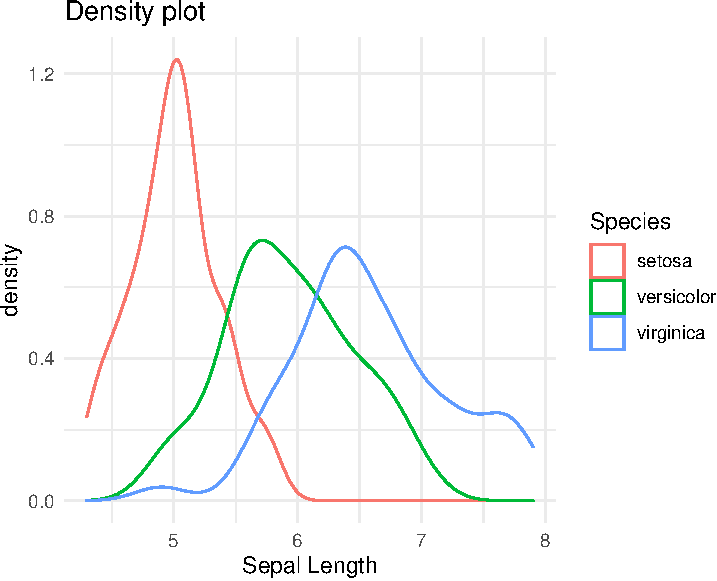
\includegraphics{visualisering_22_files/figure-latex/unnamed-chunk-140-1.pdf}

\textbf{Density plot med fill og gennemsigtig farver}

Vi kan angive en værdi for \texttt{alpha} indenfor \texttt{geom\_density()}. Den parameter \texttt{alpha} specificerer gennemsigtigheden af de density kurver i plottet.

\begin{Shaded}
\begin{Highlighting}[]
\FunctionTok{ggplot}\NormalTok{(}\AttributeTok{data=}\NormalTok{iris, }\FunctionTok{aes}\NormalTok{(}\AttributeTok{x=}\NormalTok{Sepal.Length, }\AttributeTok{fill=}\NormalTok{Species)) }\SpecialCharTok{+} 
  \FunctionTok{geom\_density}\NormalTok{(}\AttributeTok{alpha=}\FloatTok{0.5}\NormalTok{) }\SpecialCharTok{+} 
  \FunctionTok{xlab}\NormalTok{(}\StringTok{"Sepal Length"}\NormalTok{) }\SpecialCharTok{+} 
  \FunctionTok{ggtitle}\NormalTok{(}\StringTok{"Density plot with alpha=0.5"}\NormalTok{) }\SpecialCharTok{+}
  \FunctionTok{theme\_minimal}\NormalTok{()}
\end{Highlighting}
\end{Shaded}

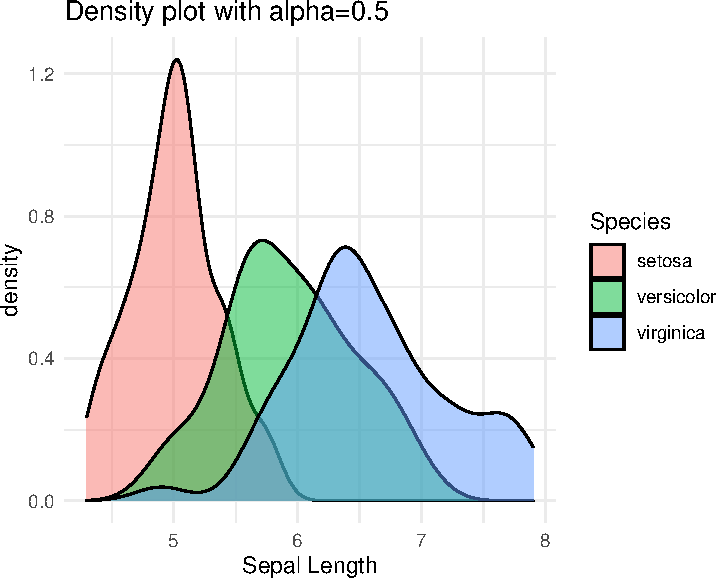
\includegraphics{visualisering_22_files/figure-latex/unnamed-chunk-141-1.pdf}

\textbf{Tilføje middelværdi linjer}

Vi bruger funktionen \texttt{tapply()} til at beregne middelværdier af \texttt{Sepal.Length} for hver af de tre \texttt{Species}. Vi kan derefter tilføje dem som lodrette linjer to vores plot. Her bruger vi \texttt{geom\_vline()} (OBS det er \texttt{geom\_hline()} hvis man vil have en vandret linje) og fortæller, at \texttt{xintercept} skal vare lig med de middelværdier, som vi har beregnet. Parameteren \texttt{lty=2} betyder, at vi vil gerne have en ``dashed'' linje.

\begin{Shaded}
\begin{Highlighting}[]
\NormalTok{means }\OtherTok{\textless{}{-}} \FunctionTok{tapply}\NormalTok{(iris}\SpecialCharTok{$}\NormalTok{Sepal.Length,iris}\SpecialCharTok{$}\NormalTok{Species,median)}

\FunctionTok{ggplot}\NormalTok{(}\AttributeTok{data=}\NormalTok{iris, }\FunctionTok{aes}\NormalTok{(}\AttributeTok{x=}\NormalTok{Sepal.Length, }\AttributeTok{color=}\NormalTok{Species)) }\SpecialCharTok{+} 
  \FunctionTok{geom\_density}\NormalTok{(}\AttributeTok{alpha=}\FloatTok{0.5}\NormalTok{) }\SpecialCharTok{+} 
  \FunctionTok{xlab}\NormalTok{(}\StringTok{"Sepal Length"}\NormalTok{) }\SpecialCharTok{+} 
  \FunctionTok{ggtitle}\NormalTok{(}\StringTok{"Density plot with alpha=0.5"}\NormalTok{) }\SpecialCharTok{+} 
  \FunctionTok{geom\_vline}\NormalTok{(}\AttributeTok{xintercept =}\NormalTok{ means,}\AttributeTok{lty=}\DecValTok{2}\NormalTok{) }\SpecialCharTok{+} 
  \FunctionTok{theme\_minimal}\NormalTok{()}
\end{Highlighting}
\end{Shaded}

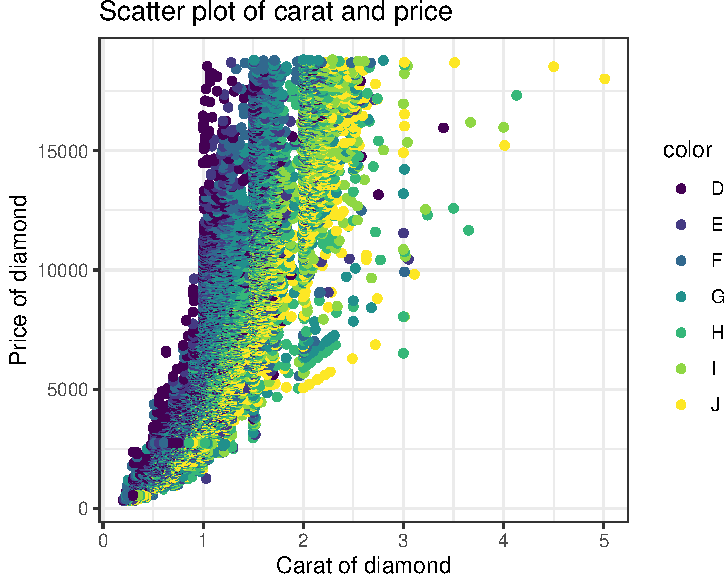
\includegraphics{visualisering_22_files/figure-latex/unnamed-chunk-142-1.pdf}

\hypertarget{troubleshooting}{%
\section{Troubleshooting}\label{troubleshooting}}

Her er en lille list over nogle ting, der forårsager en fejl når man kører kode med \textbf{ggplot2}. Jeg tilføjer også andre ting som opstå i vores lektion :).

\begin{itemize}
\item
  \texttt{ggplot(data=iris,\ aes(....))} : husk her \texttt{data=iris} er korrekt og \textbf{ikke} \texttt{Data=iris} (R skelner mellem store og små bogstaver). Man kan også undlade at bruge \texttt{data=} og skrive bare \texttt{iris} i stedet for.
\item
  Forkert stavning - dobbelt tjek, at du har stavet variabler eller funktioner navne korrekt.
\item
  Glemte \texttt{+} symbol - for at forbinde komponenterne i plottet, skal man huske at tilføje \texttt{+} i slutningen af en linje og så skrive de næste komponent bagefter (man behøver ikke at skrive hver komponent på en ny linje med det gøre det nemmere at læse koden).
\item
  Skrev \texttt{\%\textgreater{}\%} symbol i stedet for \texttt{+} - de øvrige pakker fra \textbf{tidyverse} bruger \texttt{\%\textgreater{}\%}.
\item
  Glemte parentes: her har man glemt den sidste parentes: skal være \texttt{fill=Species))} og \textbf{ikke} \texttt{fill=Species)}. Man får bare en \texttt{+} fordi R forventer at du fortsætter med at skrive mere kode.
\end{itemize}

\begin{Shaded}
\begin{Highlighting}[]
\SpecialCharTok{\textgreater{}} \FunctionTok{ggplot}\NormalTok{(}\AttributeTok{data=}\NormalTok{iris, }\FunctionTok{aes}\NormalTok{(}\AttributeTok{x=}\NormalTok{Sepal.Length, }\AttributeTok{fill=}\NormalTok{Species)}
\SpecialCharTok{+} 
\end{Highlighting}
\end{Shaded}

\begin{itemize}
\tightlist
\item
  \texttt{fill} og \texttt{colour} - indenfor \texttt{aes()} refererer \texttt{fill} til at man fylder fk. bars eller regioner med farver, og \texttt{colour} referere til farven af linjer eller punkter.
\end{itemize}

\hypertarget{problemstillinger-2}{%
\section{Problemstillinger}\label{problemstillinger-2}}

\textbf{1)} Quiz på Absalon - den hedder \texttt{Quiz\ -\ ggplot2\ part\ 1}.

\emph{OBS: Husk at lave følgende øvelser i R Markdown. Det er god praksis at sikre, at jeres dokument knitter - i selve eksamen afleverer du et html dokument.}

\begin{itemize}
\tightlist
\item
  \emph{Lav et nyt R Markdown dokument og fjern de eksempel koder. Husk at oprette en ny chunk ved at trykke på ``Insert'' new chunk", eller bruge shortcut-kommandoen CMD+ALT+I eller CTRL+ALT+I. Jeg anbefaler, at I oprette en ny chunk for hver plot, I laver}.
\end{itemize}

Vi bruger datasættet der hedder \texttt{diamonds}. Huske at først indlæse de data:*

\begin{Shaded}
\begin{Highlighting}[]
\FunctionTok{data}\NormalTok{(diamonds)}
\end{Highlighting}
\end{Shaded}

Her er beskrivelsen af \texttt{diamonds}:

\emph{Prices of over 50,000 round cut diamonds:} a dataset containing the prices and other attributes of almost 54,000 diamonds.

Se også ?diamonds for en beskrivelse af de variabler.

\textbf{2)} Bruge datasættet \texttt{diamonds} til at lave et scatter plot (\texttt{geom\_point()}):

\begin{itemize}
\tightlist
\item
  \texttt{caret} på x-aksen
\item
  \texttt{price} på y-aksen
\end{itemize}

Så at du har noget at sammenligne med, skal dit plot se sådan ud:

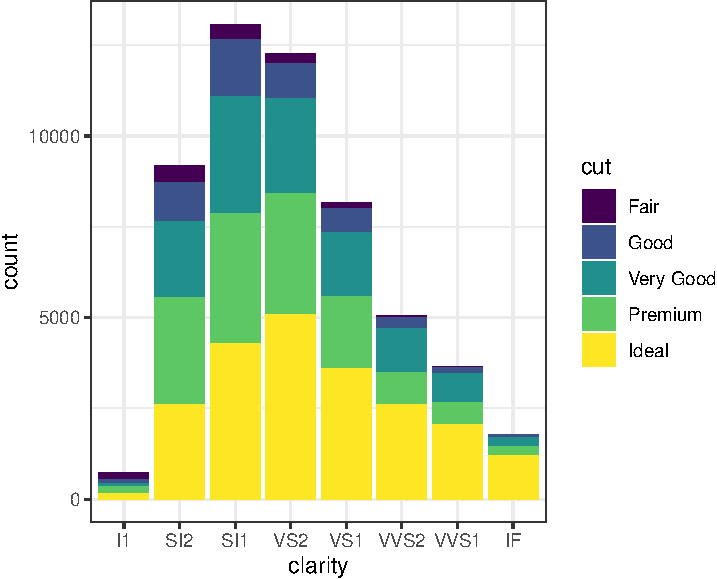
\includegraphics{visualisering_22_files/figure-latex/unnamed-chunk-145-1.pdf}

\textbf{3)} Tilføj nogle komponenter til dit plot fra \textbf{2)}.

\begin{itemize}
\tightlist
\item
  En x-akse label (\texttt{xlab()}) og en y-akse label (\texttt{ylab()})
\item
  En titel (\texttt{ggtitle()})
\item
  Et tema som hedder \texttt{theme\_bw()}
\item
  Husk at forbinde komponenterne med \texttt{+} og skrive de nye komponenter på deres egen linje.
\end{itemize}

Det skal se sådan ud:

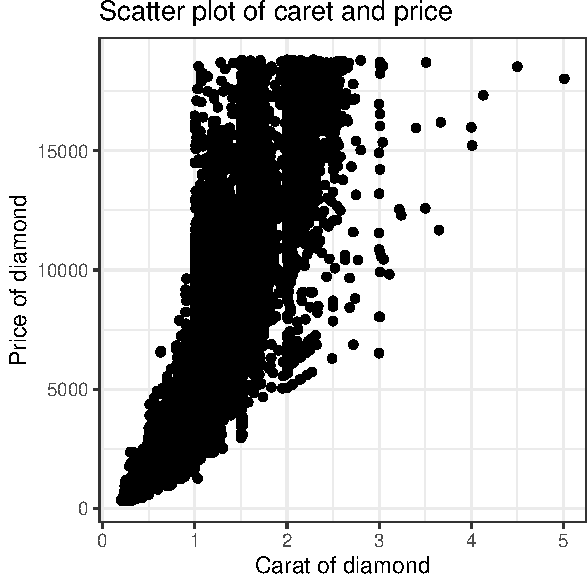
\includegraphics{visualisering_22_files/figure-latex/unnamed-chunk-146-1.pdf}

\textbf{4)} Ændre temaet af dit plot til \texttt{theme\_classic()} eller \texttt{theme\_minimal()} i stedet for \texttt{theme\_bw()} og kig på resultatet.

\begin{itemize}
\tightlist
\item
  Hvis man (måske ved uheld) skriver ind \textbf{to} temaer på samme tid (for eksempel \texttt{+\ theme\_bw()\ +\ theme\_classic()}) - hvilket tema får man så i plottet?
\item
  Valgfri ekstra: her er nogle flere tema man kan prøve: \url{https://ggplot2.tidyverse.org/reference/ggtheme.html}*
\end{itemize}

\textbf{5)} Lav det samme plot som i \textbf{3)}, og skriv \texttt{color=color} indenfor \texttt{aes()}. Den første \texttt{color} refererer til punkt farver og den anden til variablen \texttt{color} i dataframen.
Det skal se sådan ud:
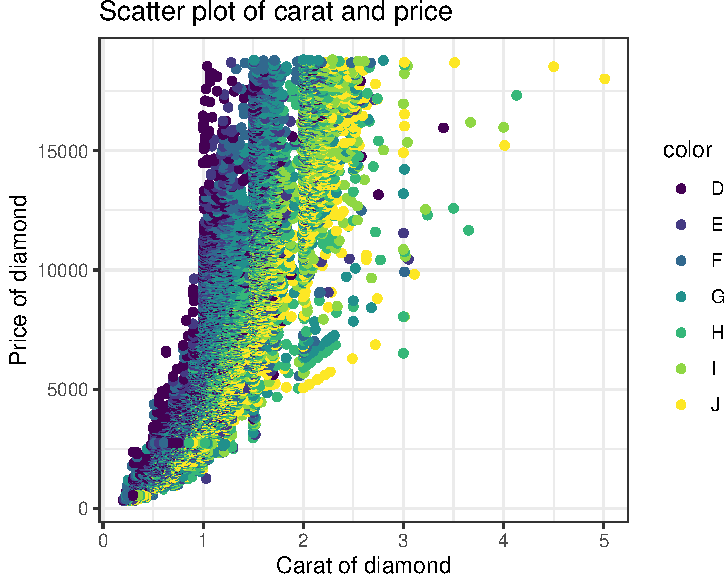
\includegraphics{visualisering_22_files/figure-latex/unnamed-chunk-147-1.pdf}

\begin{itemize}
\tightlist
\item
  Nu fjern \texttt{color=color} fra funktionen \texttt{aes()} og i stedet tilføj \texttt{aes(color=color)} i funktionen \texttt{geom\_point()}. Får du samme resultat?
\end{itemize}

\begin{itemize}
\tightlist
\item
  Bemærk at det er lige meget om man bruger britisk eller amerikansk stavning i \texttt{ggplot2} - fk. \texttt{colour} eller \texttt{color} indenfor \texttt{aes()} giiver samme resultat.
\end{itemize}

\textbf{6)} Brug stadig \texttt{diamonds}, til at lave et boxplot:

\begin{itemize}
\tightlist
\item
  \texttt{cut} på x-aksen (giv x-aksen label \texttt{Cut})
\item
  \texttt{price} på y-aksen (giv y-aksen label \texttt{Price\ of\ diamond})
\item
  bruge \texttt{fill} til at give forskellige farver til de mulige værdier af \texttt{cut}.
\item
  bruge temaet \texttt{theme\_bw()}
\end{itemize}

Det skal se sådan ud:

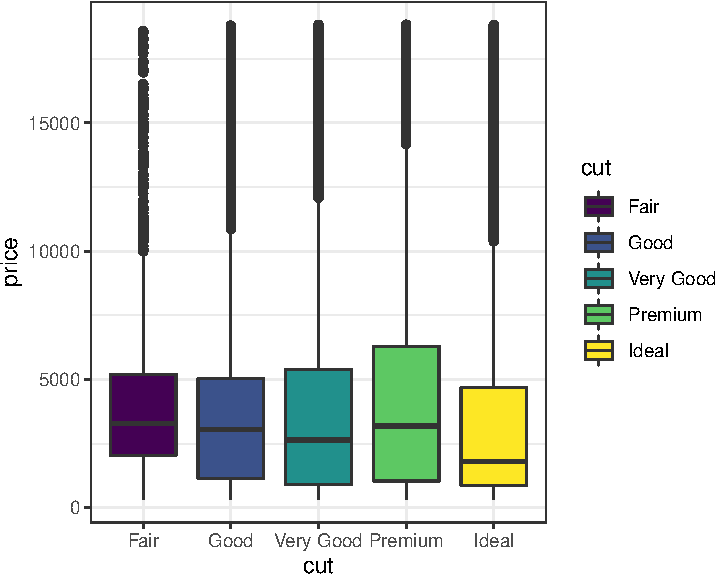
\includegraphics{visualisering_22_files/figure-latex/unnamed-chunk-148-1.pdf}

\begin{itemize}
\tightlist
\item
  Hvordan ser det ud, hvis man bruger \texttt{colour} i stedet for \texttt{fill}? Eller hvis man giver begge to?
\end{itemize}

\textbf{7)} Lav følgende ekstra ændringer til din boxplot fra ovenstående:

\begin{itemize}
\tightlist
\item
  Tilføj \texttt{geom\_jitter()} til din boxplot
\item
  fjern legend ved at tilføj \texttt{theme(legend.position="none")}
\item
  Man kan også tilføj \texttt{show.legend=FALSE} til både \texttt{geom\_boxplot()} og \texttt{geom\_jitter()} i stedet for - prøv det i stedet for at bruge \texttt{theme(legend.position="none")}. Er det nok at tilføje \texttt{show.legend=FALSE} til kun én af de to geoms?
\end{itemize}

Det skal se sådan ud:

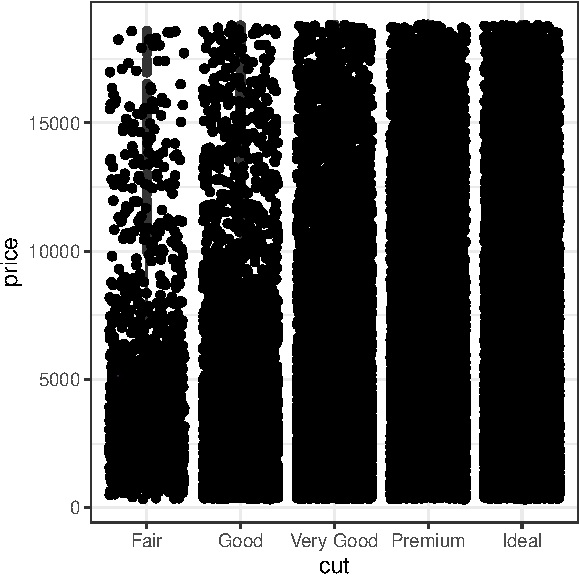
\includegraphics{visualisering_22_files/figure-latex/unnamed-chunk-149-1.pdf}

\begin{itemize}
\tightlist
\item
  Man kan også prøve at forbedre plottet ved at give nogle indstillinger ind i \texttt{geom\_jitter()}, for eksempel kan man prøve \texttt{geom\_jitter(size=.2,color="grey",alpha=0.5)} for at gøre punkter mindre overbelastende i plottet (eller kan man overvejer at fjerne dem).
\end{itemize}

Leg med de tre indstilling \texttt{size},\texttt{color} og \texttt{alpha} og ser på forskellen. Her er en note om \texttt{alpha}:

\emph{Alpha refers to the opacity of a geom. Values of alpha range from 0 to 1, with lower values corresponding to more transparent colors.} \url{https://ggplot2.tidyverse.org/reference/aes_colour_fill_alpha.html}

\begin{itemize}
\tightlist
\item
  Prøv at skifte rækkefølgerne af \texttt{geom\_jitter()} og \texttt{geom\_boxplot()} i dit plot kommando og se - gøre det en forskel til hvordan plottet ser ud?
\end{itemize}

\textbf{8)} Lav en barplot med indstillingen \texttt{stat="count"}:

\begin{itemize}
\tightlist
\item
  Variable \texttt{clarity} på x-aksen
\item
  Forskellige farver til den gruppe-variable \texttt{cut}
\item
  Specificer \texttt{position="dodge"} for at få bars ved siden af hinanden
\item
  Brug også indstillingen \texttt{colour="black"} og notater effekten
\item
  Tilføj et tema
\end{itemize}

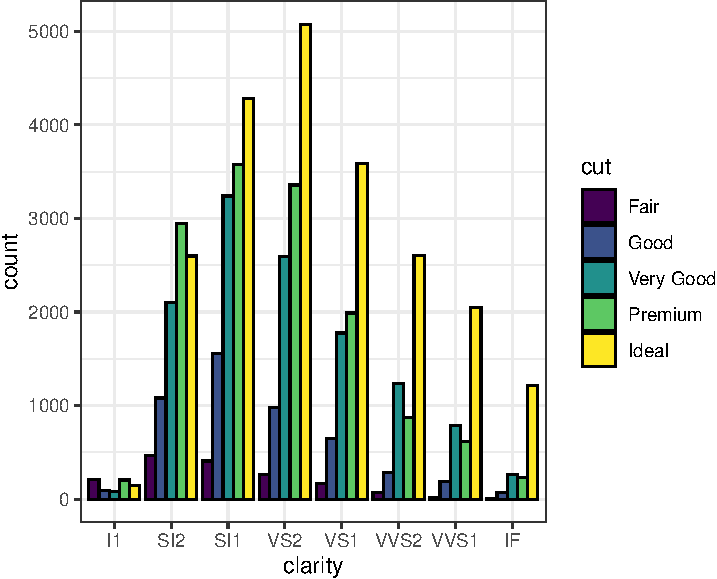
\includegraphics{visualisering_22_files/figure-latex/unnamed-chunk-150-1.pdf}

\textbf{9)} Lav en histogram

\begin{itemize}
\tightlist
\item
  Variable \texttt{depth} på x-aksen
\item
  Forskellige farver efter \texttt{cut}
\item
  Brug indstilling \texttt{alpha} til at ændre gennemsigtigheden af søljerne
\item
  Giv søjlerne en sort ramme
\item
  Tilføj et tema osv.
\end{itemize}

Det ser sådan ud:
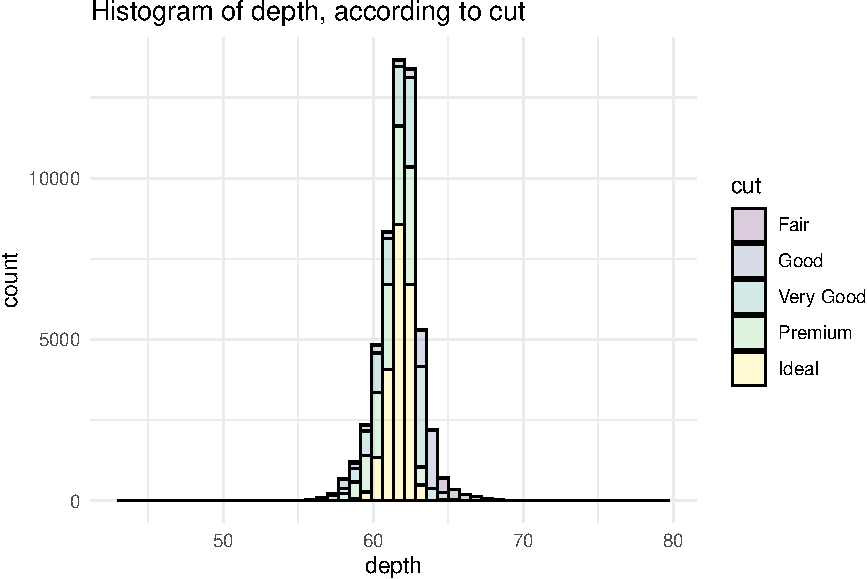
\includegraphics{visualisering_22_files/figure-latex/unnamed-chunk-151-1.pdf}

\begin{itemize}
\tightlist
\item
  Nu får du en advarsel - gør hvad advarselen siger og ændre på indstillingen \texttt{bins} indenfor \texttt{geom\_histogram()}.
\end{itemize}

\textbf{10)} Lav en density

\begin{itemize}
\tightlist
\item
  Man kan se, at det er svært at sammenligne fordelingerne i ovenstående histograms
\item
  I din histogram kode fra \textbf{9)} erstatte \texttt{geom\_histogram} med \texttt{geom\_density}
\item
  Er det nu nemmere at sammenligne fordelingerne efter de forskellige niveauer af \texttt{cut}?
\item
  Tilføj lodrette linjer med beregnede \texttt{median} værdier af variablen \texttt{depth} for hver af de cuts fra variablen \texttt{cut}.

  \begin{itemize}
  \tightlist
  \item
    Hint: \texttt{tapply} til at beregne \texttt{median}, \texttt{geom\_vline} til at lave lodrette linjer
  \end{itemize}
\end{itemize}

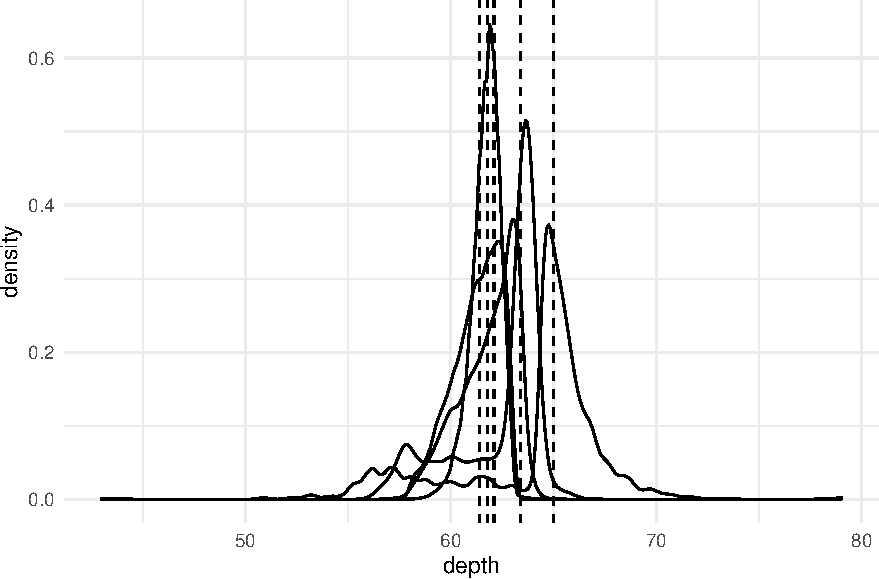
\includegraphics{visualisering_22_files/figure-latex/unnamed-chunk-152-1.pdf}

\textbf{11)} Bare ekstra øvelse: Lege frit med at lave andre plots fra \texttt{diamonds} med ggplot2. Eksempelvis

\begin{itemize}
\tightlist
\item
  Boxplots med \texttt{carat} opdelte efter \texttt{clarity}
\item
  Barplots for de forskellige farver (variable \texttt{color})
\item
  Et scatter plot af \texttt{depth} vs \texttt{price}.
\end{itemize}

I alle tilfælde tilføje akse-labs, en titel, et tema osv.

\hypertarget{nuxe6ste-gang}{%
\section{Næste gang}\label{nuxe6ste-gang}}

Efter at have lavet de problemstillinger skal man kunne se, at der er rigtig meget fleksibilitet involveret med at lave et plot med \texttt{ggplot2}. I morgen går vi videre med andre plot typer, og hvordan man fk. sætte farver manuelt.

\hypertarget{visual2}{%
\chapter{Visualisering - ggplot2 dag 2}\label{visual2}}


\includegraphics[width=2.9in]{plots/ggplot2_logo}

\hypertarget{indledning-og-videoer}{%
\section{Indledning og videoer}\label{indledning-og-videoer}}

I nuværende emne udvider du værktøjskassen af kommandoer i pakken \textbf{ggplot2} for at tillade større fleksibilitet og appel i dine visualiseringer. Jeg anbefaler, at du ser videoerne inden undervisningstimerne og bruger notaterne som en slags reference samtidig at du arbejder med problemstillingerne.

\hypertarget{luxe6ringsmuxe5lene}{%
\subsection{Læringsmålene}\label{luxe6ringsmuxe5lene}}

I skal være i stand til at:

\begin{itemize}
\tightlist
\item
  Arbejde fleksibelt med koordinat systemer - transformering, modificering og ``flipping'' af x- og y-aksen.
\item
  Udvide brugen af farver og form.
\item
  Tilføje tekst direkte på plottet med \texttt{geom\_text()}.
\item
  Bruge \texttt{facet\_grid()} eller \texttt{facet\_wrap()} til at adskille plots efter en katagorisk variabel.
\item
  Gemme dit færdigt plot i en fil.
\end{itemize}

\begin{Shaded}
\begin{Highlighting}[]
\FunctionTok{library}\NormalTok{(ggplot2) }\CommentTok{\#husk}
\end{Highlighting}
\end{Shaded}

\hypertarget{video-ressourcer-1}{%
\subsection{Video ressourcer}\label{video-ressourcer-1}}

\begin{itemize}
\tightlist
\item
  Video 1: Koordinat systemer (2021)
\end{itemize}

Link her hvis det ikke virker nedenunder: \url{https://player.vimeo.com/video/544201985}

\begin{itemize}
\tightlist
\item
  Video 2: Farver og punkt former (2021)
\end{itemize}

Link her hvis det ikke virker nedenunder: \url{https://player.vimeo.com/video/544218153}

\begin{itemize}
\tightlist
\item
  Video 3: Labels - \texttt{geom\_text()} og \texttt{geom\_text\_repel()} (2021)
\end{itemize}

Link her hvis det ikke virker nedenunder: \url{https://player.vimeo.com/video/544226498}

\begin{itemize}
\tightlist
\item
  Video 4 - Facets
\end{itemize}

Link her hvis det ikke virker nedenunder: \url{https://player.vimeo.com/video/704140333}

\hypertarget{koordinat-systemer}{%
\section{Koordinat systemer}\label{koordinat-systemer}}

Her arbejder vi videre med koordinater i pakken \textbf{ggplot2}.

\hypertarget{zoom-coord_cartesian-expand_limits}{%
\subsection{\texorpdfstring{Zoom (\texttt{coord\_cartesian()}, \texttt{expand\_limits()})}{Zoom (coord\_cartesian(), expand\_limits())}}\label{zoom-coord_cartesian-expand_limits}}

Man kan bruge funktionen \texttt{coord\_cartesian()} til at zoome ind på et bestemt område i plottet. \textbf{Indenfor} \texttt{coord\_cartesian()} angives \texttt{xlim()} og \texttt{ylim()}, som specificerer de øvre og nedre grænser langt henholdsvis x-aksen og y-aksen. Man kan også bruge \texttt{xlim()} og \texttt{ylim()} udenom \texttt{coord\_cartesian()}, men i dette tilfælde bliver punkterne, som ikke kan ses i plottet (fordi deres koordinater ligger udenfor de angivne grænser), smidt væk (med en advarsel). Med \texttt{coord\_cartesian()} beholder man til gengæld samtlige data, og man får således ikke en advarsel.

I følgende ses vores oprindeligt scatter plot:

\begin{Shaded}
\begin{Highlighting}[]
\FunctionTok{ggplot}\NormalTok{(iris, }\FunctionTok{aes}\NormalTok{(}\AttributeTok{x =}\NormalTok{ Sepal.Length, }\AttributeTok{y =}\NormalTok{ Sepal.Width,}\AttributeTok{color =}\NormalTok{ Species)) }\SpecialCharTok{+}
  \FunctionTok{geom\_point}\NormalTok{() }\SpecialCharTok{+} 
  \FunctionTok{theme\_minimal}\NormalTok{() }
\end{Highlighting}
\end{Shaded}

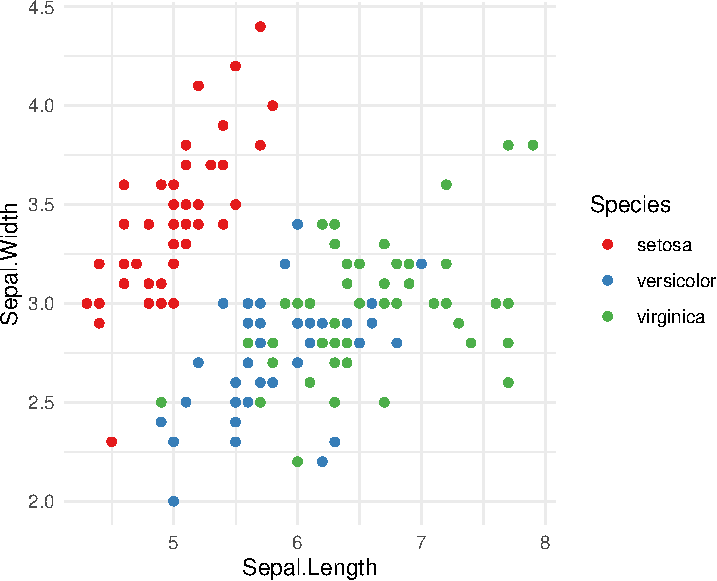
\includegraphics{visualisering_22_files/figure-latex/unnamed-chunk-159-1.pdf}

Og her anvender jeg funktionen \texttt{coord\_cartesian()} med \texttt{xlim()} og \texttt{ylim()} indenfor til at zoome ind på et ønsket område på plottet.

\begin{Shaded}
\begin{Highlighting}[]
\FunctionTok{ggplot}\NormalTok{(iris, }\FunctionTok{aes}\NormalTok{(}\AttributeTok{x =}\NormalTok{ Sepal.Length, }\AttributeTok{y =}\NormalTok{ Sepal.Width,}\AttributeTok{color =}\NormalTok{ Species)) }\SpecialCharTok{+}
  \FunctionTok{geom\_point}\NormalTok{() }\SpecialCharTok{+} 
  \FunctionTok{coord\_cartesian}\NormalTok{(}\AttributeTok{xlim =} \FunctionTok{c}\NormalTok{(}\DecValTok{4}\NormalTok{,}\DecValTok{6}\NormalTok{), }\AttributeTok{ylim =} \FunctionTok{c}\NormalTok{(}\FloatTok{2.2}\NormalTok{,}\FloatTok{4.5}\NormalTok{)) }\SpecialCharTok{+}
  \FunctionTok{theme\_minimal}\NormalTok{() }
\end{Highlighting}
\end{Shaded}

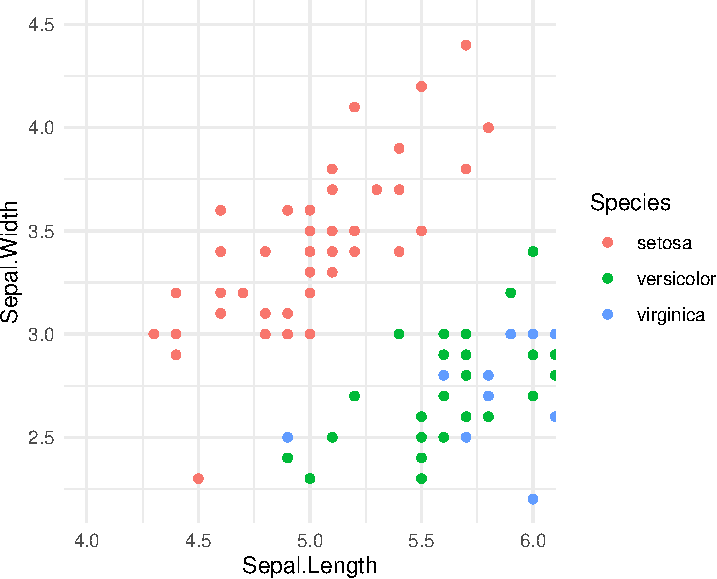
\includegraphics{visualisering_22_files/figure-latex/unnamed-chunk-160-1.pdf}

Du kan også zoome ud ved at bruge \texttt{expand\_limits()}. For eksempel hvis jeg gerne vil have punkterne \(x = 0\) og \(y = 0\) (\texttt{c(0,0)}, eller ``origin'') med i selve plottet:

\begin{Shaded}
\begin{Highlighting}[]
\FunctionTok{ggplot}\NormalTok{(iris, }\FunctionTok{aes}\NormalTok{(}\AttributeTok{x=}\NormalTok{Sepal.Length, }\AttributeTok{y=}\NormalTok{Sepal.Width,}\AttributeTok{col=}\NormalTok{Species)) }\SpecialCharTok{+}
  \FunctionTok{geom\_point}\NormalTok{() }\SpecialCharTok{+} 
  \FunctionTok{expand\_limits}\NormalTok{(}\AttributeTok{x =} \DecValTok{0}\NormalTok{, }\AttributeTok{y =} \DecValTok{0}\NormalTok{) }\SpecialCharTok{+}
  \FunctionTok{theme\_minimal}\NormalTok{() }
\end{Highlighting}
\end{Shaded}

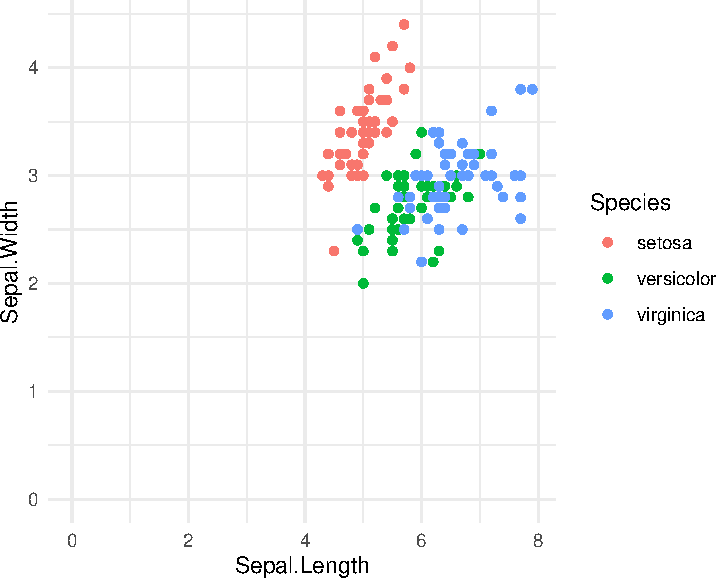
\includegraphics{visualisering_22_files/figure-latex/unnamed-chunk-161-1.pdf}

Det kan være brubart i situationer hvor man, eksempelvis har flere etiketter omkring punkterne i selve plottet, som bedre kan ses hvis man tillader lidt ekstra plads i plottets område.

\hypertarget{transformering-af-akserne---log-sqrt-osv-scale_x_continuous.}{%
\subsection{\texorpdfstring{Transformering af akserne - log, sqrt osv (\texttt{scale\_x\_continuous}).}{Transformering af akserne - log, sqrt osv (scale\_x\_continuous).}}\label{transformering-af-akserne---log-sqrt-osv-scale_x_continuous.}}

Nogle gange kan det være svært at visualisere nogle variabler på grund af deres fordeling. Er der mange outliers i variablen så er de fleste punkter samlede i et lille område i plottet. Transformering med enten \texttt{log} eller \texttt{sqrt} på x-aksen og/eller y-aksen er især en populær tilgang, så de data kan ses på en mere informativ måde.

\begin{Shaded}
\begin{Highlighting}[]
\FunctionTok{ggplot}\NormalTok{(iris, }\FunctionTok{aes}\NormalTok{(}\AttributeTok{x=}\NormalTok{Sepal.Length, }\AttributeTok{y=}\NormalTok{Sepal.Width,}\AttributeTok{col=}\NormalTok{Species)) }\SpecialCharTok{+}
  \FunctionTok{geom\_point}\NormalTok{(}\AttributeTok{size=}\DecValTok{3}\NormalTok{) }\SpecialCharTok{+} 
  \FunctionTok{scale\_x\_continuous}\NormalTok{(}\AttributeTok{trans =} \StringTok{"log2"}\NormalTok{) }\SpecialCharTok{+}
  \FunctionTok{scale\_y\_continuous}\NormalTok{(}\AttributeTok{trans =} \StringTok{"log2"}\NormalTok{) }\SpecialCharTok{+}
  \FunctionTok{theme\_minimal}\NormalTok{() }
\end{Highlighting}
\end{Shaded}

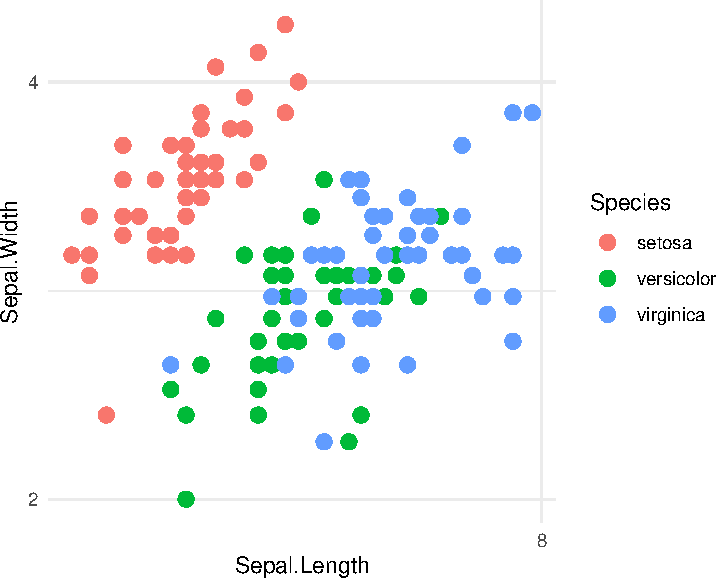
\includegraphics{visualisering_22_files/figure-latex/unnamed-chunk-162-1.pdf}

Man kan også prøve fk. ``sqrt'' i stedet for ``log2''. Formålet er, at hvis de data fordeler sig mere `normalt', kan man nemmere visualiser det i et plot - en måde til at gøre der er ved at transformere de data med ``sqrt'' eller ``log2''.

Bemærk at det er til forskel fra at man transformere selve data som bruges i plottet. Jeg kan for eksempel få samme resultat ved at ændre på datasættet forud for at anvende \texttt{ggplot2} - her behøver jeg ikke at bruge \texttt{scale\_x\_continuous(trans\ =\ "log2")} for at opnår samme resultat, men notater at tallerne på akserne reflektere de transformeret data og ikke de oprindelige værdier. Den beslutninger man tager her kommer an på, hvad man gerne vil opnå med analysering af de data.

\begin{Shaded}
\begin{Highlighting}[]
\NormalTok{iris}\SpecialCharTok{$}\NormalTok{Sepal.Length }\OtherTok{\textless{}{-}} \FunctionTok{log2}\NormalTok{(iris}\SpecialCharTok{$}\NormalTok{Sepal.Length)}
\NormalTok{iris}\SpecialCharTok{$}\NormalTok{Sepal.Width }\OtherTok{\textless{}{-}} \FunctionTok{log2}\NormalTok{(iris}\SpecialCharTok{$}\NormalTok{Sepal.Width)}
\FunctionTok{ggplot}\NormalTok{(iris, }\FunctionTok{aes}\NormalTok{(}\AttributeTok{x=}\NormalTok{Sepal.Length, }\AttributeTok{y=}\NormalTok{Sepal.Width,}\AttributeTok{col=}\NormalTok{Species)) }\SpecialCharTok{+}
  \FunctionTok{geom\_point}\NormalTok{(}\AttributeTok{size=}\DecValTok{3}\NormalTok{) }\SpecialCharTok{+}
  \FunctionTok{theme\_minimal}\NormalTok{() }
\end{Highlighting}
\end{Shaded}

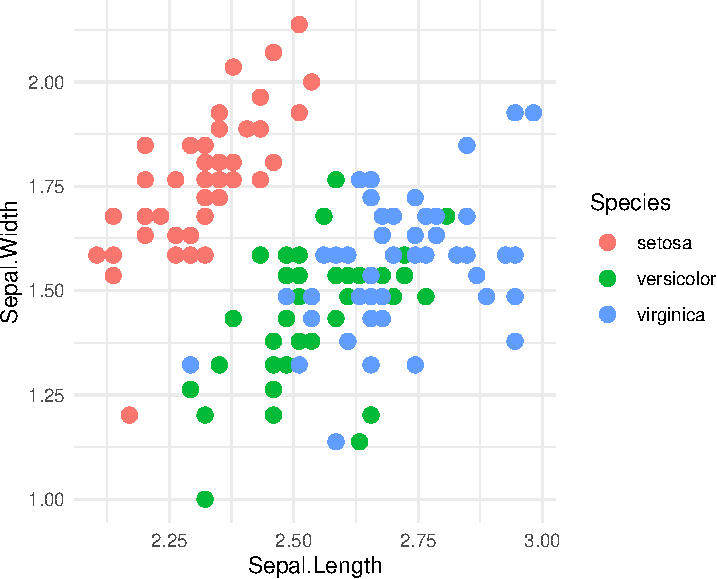
\includegraphics{visualisering_22_files/figure-latex/unnamed-chunk-163-1.pdf}

\hypertarget{flip-coordinates-coord_flip}{%
\subsection{\texorpdfstring{Flip coordinates (\texttt{coord\_flip})}{Flip coordinates (coord\_flip)}}\label{flip-coordinates-coord_flip}}

Vi kan bruge \texttt{coord\_flip()} til at spejler x-aksen på y-aksen og omvendt (det svarer til, at man drejer plottet ved 90 grader). Se følgende eksempel, hvor jeg først opretter variablen \texttt{Sepal.Group}, laver en barplot og anvender \texttt{coord\_flip} for at få vandrettet søjler.

\begin{Shaded}
\begin{Highlighting}[]
\CommentTok{\#Sepal.Group defineret som i går}
\NormalTok{iris}\SpecialCharTok{$}\NormalTok{Sepal.Group }\OtherTok{\textless{}{-}} \FunctionTok{ifelse}\NormalTok{(iris}\SpecialCharTok{$}\NormalTok{Sepal.Length}\SpecialCharTok{\textgreater{}}\FunctionTok{mean}\NormalTok{(iris}\SpecialCharTok{$}\NormalTok{Sepal.Length),}\StringTok{"Long"}\NormalTok{,}\StringTok{"Short"}\NormalTok{)}

\FunctionTok{ggplot}\NormalTok{(iris,}\FunctionTok{aes}\NormalTok{(}\AttributeTok{x=}\NormalTok{Species,}\AttributeTok{fill=}\NormalTok{Sepal.Group)) }\SpecialCharTok{+} 
  \FunctionTok{geom\_bar}\NormalTok{(}\AttributeTok{stat=}\StringTok{"count"}\NormalTok{,}\AttributeTok{position=}\StringTok{"dodge"}\NormalTok{,}\AttributeTok{color=}\StringTok{"black"}\NormalTok{) }\SpecialCharTok{+}
  \FunctionTok{coord\_flip}\NormalTok{() }\SpecialCharTok{+}
  \FunctionTok{theme\_minimal}\NormalTok{()}
\end{Highlighting}
\end{Shaded}

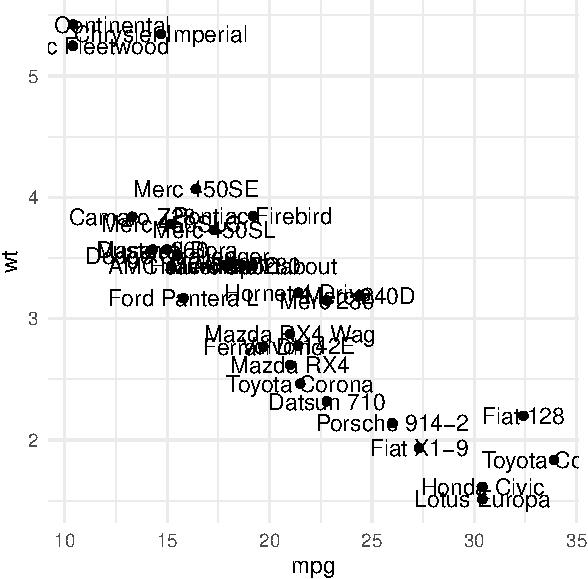
\includegraphics{visualisering_22_files/figure-latex/unnamed-chunk-164-1.pdf}

Man kan ændre på rækkefølgen af de tre \texttt{Species} ved at bruge funktionen \texttt{scale\_x\_discrete()} og angiver den nye rækkefølge med indstillingen \texttt{limits}:

\begin{Shaded}
\begin{Highlighting}[]
\FunctionTok{ggplot}\NormalTok{(iris,}\FunctionTok{aes}\NormalTok{(}\AttributeTok{x=}\NormalTok{Species,}\AttributeTok{fill=}\NormalTok{Sepal.Group)) }\SpecialCharTok{+} 
  \FunctionTok{geom\_bar}\NormalTok{(}\AttributeTok{stat=}\StringTok{"count"}\NormalTok{,}\AttributeTok{position=}\StringTok{"dodge"}\NormalTok{,}\AttributeTok{color=}\StringTok{"black"}\NormalTok{) }\SpecialCharTok{+}
  \FunctionTok{coord\_flip}\NormalTok{() }\SpecialCharTok{+}
  \FunctionTok{scale\_x\_discrete}\NormalTok{(}\AttributeTok{limits =} \FunctionTok{c}\NormalTok{(}\StringTok{"virginica"}\NormalTok{, }\StringTok{"versicolor"}\NormalTok{,}\StringTok{"setosa"}\NormalTok{)) }\SpecialCharTok{+}
  \FunctionTok{theme\_minimal}\NormalTok{()}
\end{Highlighting}
\end{Shaded}

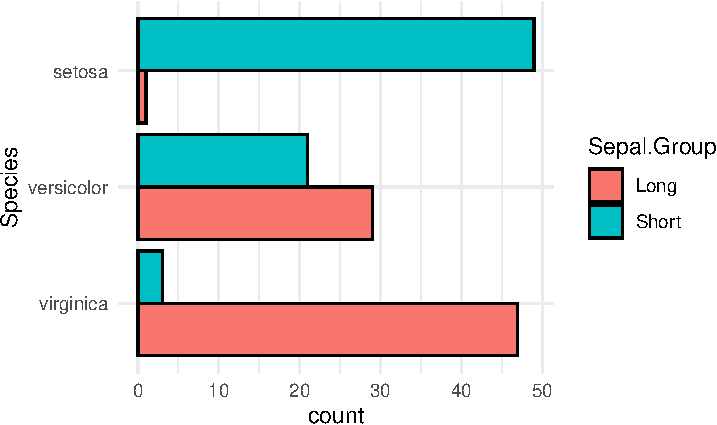
\includegraphics{visualisering_22_files/figure-latex/unnamed-chunk-165-1.pdf}

\hypertarget{mere-om-farver-og-punkt-former}{%
\section{Mere om farver og punkt former}\label{mere-om-farver-og-punkt-former}}

Der er flere måder at specificere farver på i \texttt{ggplot2}. Man kan nøjes med den automatiske løsning, som er hurtigt (og effektiv i mange situationer), eller man kan bruge den manuelle løsning, som tager lidt mere tid at indkode men er brugbar hvis man gerne vil lave et plot til at præsentere til andre.

\hypertarget{automatisk-farver}{%
\subsection{Automatisk farver}\label{automatisk-farver}}

Vi så sidste emnet at man automatisk kan bede om forskellige farver, ved at benytte \texttt{colour=Species} indenfor \texttt{aes()} i den \texttt{ggplot()} funktion.

\begin{Shaded}
\begin{Highlighting}[]
\CommentTok{\#automatisk løsning}
\FunctionTok{ggplot}\NormalTok{(iris, }\FunctionTok{aes}\NormalTok{(}\AttributeTok{x=}\NormalTok{Sepal.Length, }\AttributeTok{y=}\NormalTok{Sepal.Width, }\AttributeTok{colour=}\NormalTok{Species)) }\SpecialCharTok{+}
  \FunctionTok{geom\_point}\NormalTok{() }\SpecialCharTok{+}
  \FunctionTok{theme\_minimal}\NormalTok{() }
\end{Highlighting}
\end{Shaded}

\includegraphics{visualisering_22_files/figure-latex/unnamed-chunk-166-1.pdf}

\hypertarget{manuelle-farver}{%
\subsection{Manuelle farver}\label{manuelle-farver}}

Hvis man foretrækker at bruge sine egne farver, kan man det ved at benytte funktionen \texttt{scale\_colour\_manual()}. Her angiver jeg stadig \texttt{colour=Species} indenfor \texttt{aes()} men så angiver jeg hvilke bestemte farver de forskellige arter skal få indenfor \texttt{scale\_colour\_manual} med indstillingen \texttt{values}.

\begin{Shaded}
\begin{Highlighting}[]
\CommentTok{\#manuelt løsning}
\FunctionTok{ggplot}\NormalTok{(iris, }\FunctionTok{aes}\NormalTok{(}\AttributeTok{x=}\NormalTok{Sepal.Length, }\AttributeTok{y=}\NormalTok{Sepal.Width, }\AttributeTok{colour=}\NormalTok{Species)) }\SpecialCharTok{+}
  \FunctionTok{scale\_colour\_manual}\NormalTok{(}\AttributeTok{values=}\FunctionTok{c}\NormalTok{(}\StringTok{"purple"}\NormalTok{, }\StringTok{"yellow"}\NormalTok{,}\StringTok{"pink"}\NormalTok{)) }\SpecialCharTok{+}
  \FunctionTok{geom\_point}\NormalTok{() }\SpecialCharTok{+}
  \FunctionTok{theme\_minimal}\NormalTok{() }
\end{Highlighting}
\end{Shaded}

\includegraphics{visualisering_22_files/figure-latex/unnamed-chunk-167-1.pdf}

En faktastisk pakke er \texttt{RColorBrewer}. Pakken indeholder mange forskellige ``colour palettes'', det vil sige grupper af farver, der passer godt med hinanden. Man kan således slippe for at selv samle et godt kombination der passer til plottet. Nogle af de colour palettes tager også i betragtning, eksempelvis hvis man er farveblind, eller om man vil have en farvegradient eller et sæt diskrete farver som ikke ligner hinanden.

I følgende indlæser jeg pakken \texttt{RColorBrewer} og anvender funktionen \texttt{scale\_colour\_brewer} med indstillingen \texttt{palette="Set1"}:

\begin{Shaded}
\begin{Highlighting}[]
\CommentTok{\#install.packages("RColorBrewer")}
\FunctionTok{library}\NormalTok{(RColorBrewer)}

\CommentTok{\#manuelt løsning}
\FunctionTok{ggplot}\NormalTok{(iris, }\FunctionTok{aes}\NormalTok{(}\AttributeTok{x=}\NormalTok{Sepal.Length, }\AttributeTok{y=}\NormalTok{Sepal.Width, }\AttributeTok{colour=}\NormalTok{Species)) }\SpecialCharTok{+}
  \FunctionTok{scale\_colour\_brewer}\NormalTok{(}\AttributeTok{palette=}\StringTok{"Set1"}\NormalTok{) }\SpecialCharTok{+}
  \FunctionTok{geom\_point}\NormalTok{() }\SpecialCharTok{+}
  \FunctionTok{theme\_minimal}\NormalTok{() }
\end{Highlighting}
\end{Shaded}

\includegraphics{visualisering_22_files/figure-latex/unnamed-chunk-168-1.pdf}

Bemærk at både \texttt{scale\_color\_maual()} og \texttt{scale\_color\_brewer()} sætter farver af punkter og linjer, mens i en boxplot eller barplot sammenhænge, bruger man \texttt{scale\_fill\_manual()} eller \texttt{scale\_fill\_brewer()}. For eksempel i følgende vil jeg gerne sætte farver på de opfyldte områder i en boxplot:

\begin{Shaded}
\begin{Highlighting}[]
\FunctionTok{ggplot}\NormalTok{(iris,}\FunctionTok{aes}\NormalTok{(}\AttributeTok{x=}\NormalTok{Species,}\AttributeTok{y=}\NormalTok{Sepal.Length,}\AttributeTok{fill=}\NormalTok{Species)) }\SpecialCharTok{+} 
  \FunctionTok{geom\_boxplot}\NormalTok{() }\SpecialCharTok{+}
  \FunctionTok{scale\_fill\_brewer}\NormalTok{(}\AttributeTok{palette=}\StringTok{"Set2"}\NormalTok{)  }\SpecialCharTok{+} 
  \FunctionTok{theme\_minimal}\NormalTok{()}
\end{Highlighting}
\end{Shaded}

\includegraphics{visualisering_22_files/figure-latex/unnamed-chunk-169-1.pdf}

Her er en oversigt over de fire funktioner.

\begin{longtable}[]{@{}
  >{\raggedright\arraybackslash}p{(\columnwidth - 2\tabcolsep) * \real{0.50}}
  >{\raggedright\arraybackslash}p{(\columnwidth - 2\tabcolsep) * \real{0.50}}@{}}
\toprule
fuktion & beskrivelse \\
\midrule
\endhead
\texttt{scale\_fill\_manual(values=c("firebrick3","blue"))} & manuelle farver til boxplots og barplots osv. \\
\texttt{scale\_color\_maual(values=c("darkorchid","cyan4"))} & manulle farver til punkter og linjer osv. \\
\texttt{scale\_fill\_brewer(palette="Dark2")} & \texttt{RColourBrewer} løsning til boxplots/barplots/osv. \\
\texttt{scale\_color\_brewer(palette="Set1")} & \texttt{RColourBrewer} løsning til punkter og linjer osv. \\
\bottomrule
\end{longtable}

Der er også andre muligheder hvis man har behov for dem - for eksempel for kontinuitet data kan man prøve at google efter \texttt{scale\_fill\_gradient}.

\textbf{\emph{Farver i RColourBrewer}}

Her er en nyttig reference, der viser de forskellige farver tilgængelige i pakken \texttt{RColourBrewer}.

\begin{figure}
\centering
\includegraphics{plots/rcolorbrewer.png}
\caption{Mulige colour palettes tilgængelige i RColourBrewer}
\end{figure}

\hypertarget{punkt-former}{%
\subsection{Punkt former}\label{punkt-former}}

Ligesom man kan lave forskellige farver, kan man også lave forskellige punkt former. Vi starter med den automatiske løsning ligesom vi gjorde med farver. Når det er en variable vi angiver, skal variablenavnet skrives indenfor \texttt{aes()}. Her, da \texttt{shape} er en parameter som er meget specifik til \texttt{geom\_point}, vælger jeg at skrive en ny \texttt{aes()} indenfor \texttt{geom\_point()} i stedet for indenfor funktionen \texttt{ggplot()}. Husk, at i funktionen \texttt{ggplot()} specificerer man globale ting som gælder for hele plot, og i funktionen \texttt{geom\_pont()} angiver man ting som gælder kun for \texttt{geom\_point()}. Se følgende eksempel:

\begin{Shaded}
\begin{Highlighting}[]
\FunctionTok{ggplot}\NormalTok{(}\AttributeTok{data=}\NormalTok{iris, }\FunctionTok{aes}\NormalTok{(}\AttributeTok{x =}\NormalTok{ Sepal.Length, }\AttributeTok{y =}\NormalTok{ Sepal.Width)) }\SpecialCharTok{+}
  \FunctionTok{scale\_color\_brewer}\NormalTok{(}\AttributeTok{palette=}\StringTok{"Set2"}\NormalTok{) }\SpecialCharTok{+}
  \FunctionTok{geom\_point}\NormalTok{(}\FunctionTok{aes}\NormalTok{(}\AttributeTok{shape=}\NormalTok{Species)) }\SpecialCharTok{+} 
  \FunctionTok{theme\_minimal}\NormalTok{()}
\end{Highlighting}
\end{Shaded}

\includegraphics{visualisering_22_files/figure-latex/unnamed-chunk-170-1.pdf}

Så har jeg fået både en farve og en punkt form til hver art i variablen \texttt{Species}.

\textbf{\emph{Sætte punkt form manuelt}}

Hvis vi ikke kan lide de tre punkt former vi få automatisk, kan vi ændre dem ved at bruge \texttt{scale\_shape\_manual} - her vælger jeg \texttt{values=c(1,2,3)}, men der er en reference nedenunder, hvor I kan se, de mappings mellem de numeriske tal og de punkt former, så at I kan vælger jeres egne.

\begin{Shaded}
\begin{Highlighting}[]
\FunctionTok{ggplot}\NormalTok{(}\AttributeTok{data=}\NormalTok{iris, }\FunctionTok{aes}\NormalTok{(}\AttributeTok{x =}\NormalTok{ Sepal.Length, }\AttributeTok{y =}\NormalTok{ Sepal.Width, }\AttributeTok{colour=}\NormalTok{Species)) }\SpecialCharTok{+}
  \FunctionTok{geom\_point}\NormalTok{(}\FunctionTok{aes}\NormalTok{(}\AttributeTok{shape=}\NormalTok{Species)) }\SpecialCharTok{+} 
  \FunctionTok{scale\_color\_brewer}\NormalTok{(}\AttributeTok{palette=}\StringTok{"Set2"}\NormalTok{) }\SpecialCharTok{+}
  \FunctionTok{scale\_shape\_manual}\NormalTok{(}\AttributeTok{values=}\FunctionTok{c}\NormalTok{(}\DecValTok{1}\NormalTok{,}\DecValTok{2}\NormalTok{,}\DecValTok{3}\NormalTok{)) }\SpecialCharTok{+}
  \FunctionTok{theme\_minimal}\NormalTok{()}
\end{Highlighting}
\end{Shaded}

\includegraphics{visualisering_22_files/figure-latex/unnamed-chunk-171-1.pdf}

\textbf{\emph{Reference for punkt former}}

\includegraphics{visualisering_22_files/figure-latex/unnamed-chunk-172-1.pdf}

\hypertarget{annotations-geom_text}{%
\section{\texorpdfstring{Annotations (\texttt{geom\_text})}{Annotations (geom\_text)}}\label{annotations-geom_text}}

\hypertarget{tilfuxf8je-labeller-direkte-puxe5-plottet.}{%
\subsection{Tilføje labeller direkte på plottet.}\label{tilfuxf8je-labeller-direkte-puxe5-plottet.}}

Man kan bruge \texttt{geom\_text()} til at tilføje tekst på punkterne direkte på plottet. Her skal man fortælle, hvad for nogle tekst skal være på plottet - her specificerer vi navne på biler fra datasættet \texttt{mtcars}. Plottet er en scatter plot mellem variabler \texttt{mpg} og \texttt{wt}.

\begin{Shaded}
\begin{Highlighting}[]
\FunctionTok{data}\NormalTok{(mtcars)}

\NormalTok{mtcars}\SpecialCharTok{$}\NormalTok{my\_labels }\OtherTok{\textless{}{-}} \FunctionTok{row.names}\NormalTok{(mtcars) }\CommentTok{\#take row names and set as a variable}

\FunctionTok{ggplot}\NormalTok{(mtcars,}\FunctionTok{aes}\NormalTok{(}\AttributeTok{x=}\NormalTok{mpg,}\AttributeTok{y=}\NormalTok{wt)) }\SpecialCharTok{+} 
  \FunctionTok{geom\_point}\NormalTok{() }\SpecialCharTok{+}
  \FunctionTok{geom\_text}\NormalTok{(}\FunctionTok{aes}\NormalTok{(}\AttributeTok{label=}\NormalTok{my\_labels)) }\SpecialCharTok{+} 
  \FunctionTok{theme\_minimal}\NormalTok{()}
\end{Highlighting}
\end{Shaded}

\includegraphics{visualisering_22_files/figure-latex/unnamed-chunk-173-1.pdf}

For at gøre det nemmere at læse kan man også fjerne selve punkterne:

\begin{Shaded}
\begin{Highlighting}[]
\FunctionTok{ggplot}\NormalTok{(mtcars,}\FunctionTok{aes}\NormalTok{(}\AttributeTok{x=}\NormalTok{mpg,}\AttributeTok{y=}\NormalTok{wt)) }\SpecialCharTok{+} 
  \CommentTok{\#geom\_point() +}
  \FunctionTok{geom\_text}\NormalTok{(}\FunctionTok{aes}\NormalTok{(}\AttributeTok{label=}\NormalTok{my\_labels)) }\SpecialCharTok{+} 
  \FunctionTok{theme\_minimal}\NormalTok{()}
\end{Highlighting}
\end{Shaded}

\includegraphics{visualisering_22_files/figure-latex/unnamed-chunk-174-1.pdf}

Teksten på plottet er stadig meget svært at læse. En god løsning kan være at bruge R-pakken \texttt{ggrepel}, som i følgende.

\hypertarget{pakken-ggrepel-for-at-tilfuxf8je-tekst-labeller}{%
\subsection{\texorpdfstring{Pakken \texttt{ggrepel} for at tilføje tekst labeller}{Pakken ggrepel for at tilføje tekst labeller}}\label{pakken-ggrepel-for-at-tilfuxf8je-tekst-labeller}}

\begin{Shaded}
\begin{Highlighting}[]
\CommentTok{\#install.packages(ggrepel) \#installere hvis nødvendeigt}
\end{Highlighting}
\end{Shaded}

For at anvende pakken \texttt{ggrepel} for det \texttt{mtcars} datasæt, erstatter man bare \texttt{geom\_text()} med \texttt{geom\_text\_repel()}:

\begin{Shaded}
\begin{Highlighting}[]
\FunctionTok{library}\NormalTok{(ggrepel)}
\FunctionTok{ggplot}\NormalTok{(mtcars,}\FunctionTok{aes}\NormalTok{(}\AttributeTok{x=}\NormalTok{mpg,}\AttributeTok{y=}\NormalTok{wt)) }\SpecialCharTok{+} 
  \FunctionTok{geom\_point}\NormalTok{() }\SpecialCharTok{+}
  \FunctionTok{geom\_text\_repel}\NormalTok{(}\FunctionTok{aes}\NormalTok{(}\AttributeTok{label=}\NormalTok{my\_labels)) }\SpecialCharTok{+} 
  \FunctionTok{theme\_minimal}\NormalTok{()}
\end{Highlighting}
\end{Shaded}

\begin{verbatim}
## Warning: ggrepel: 9 unlabeled data points (too many overlaps). Consider
## increasing max.overlaps
\end{verbatim}

\includegraphics{visualisering_22_files/figure-latex/unnamed-chunk-176-1.pdf}

Så kan vi se, at nu er der ingen navne som sidder lige overfor hinanden, fordi \texttt{ggrepel()} har været dygtig nok til at placerer dem tæt på deres tilhørende punkter, og ikke ovenpå hinanden. Man kan også se her, at der er nogle punkter, hvor funktionen har tilføjet en linje for at gøre det klart, hvilken punkt teksten referer til.

I ovenstående har jeg fået en advarsel. Jeg prøver hvad jeg er blevet bedt om - og fortæller, at jeg vil have \texttt{max.overlaps\ =\ 20}.

\begin{Shaded}
\begin{Highlighting}[]
\FunctionTok{library}\NormalTok{(ggrepel)}
\FunctionTok{ggplot}\NormalTok{(mtcars,}\FunctionTok{aes}\NormalTok{(}\AttributeTok{x=}\NormalTok{mpg,}\AttributeTok{y=}\NormalTok{wt)) }\SpecialCharTok{+} 
  \FunctionTok{geom\_point}\NormalTok{() }\SpecialCharTok{+}
  \FunctionTok{geom\_text\_repel}\NormalTok{(}\FunctionTok{aes}\NormalTok{(}\AttributeTok{label=}\NormalTok{my\_labels),}\AttributeTok{max.overlaps =} \DecValTok{20}\NormalTok{) }\SpecialCharTok{+}
  \FunctionTok{theme\_minimal}\NormalTok{()}
\end{Highlighting}
\end{Shaded}

\includegraphics{visualisering_22_files/figure-latex/unnamed-chunk-177-1.pdf}

Så kan du se, at jeg ikke længere få en advarsel, og der tilhører tekst til alle punkterne nu.

\hypertarget{tilfuxf8je-rektangler-i-regioner-af-interesse-annotate}{%
\subsection{\texorpdfstring{Tilføje rektangler i regioner af interesse (\texttt{annotate})}{Tilføje rektangler i regioner af interesse (annotate)}}\label{tilfuxf8je-rektangler-i-regioner-af-interesse-annotate}}

Hvis man gerne vil fremhæve et bestemt område i plottet, kan man bruge funktionen \texttt{annotate()}. Prøve at selv regne ud, hvad de indstillinger indenfor \texttt{annotate()} gå ud på i følgende eksempel:

\begin{Shaded}
\begin{Highlighting}[]
\FunctionTok{ggplot}\NormalTok{(mtcars,}\FunctionTok{aes}\NormalTok{(}\AttributeTok{x=}\NormalTok{mpg,}\AttributeTok{y=}\NormalTok{wt)) }\SpecialCharTok{+} 
  \FunctionTok{geom\_point}\NormalTok{() }\SpecialCharTok{+}
  \FunctionTok{geom\_text\_repel}\NormalTok{(}\FunctionTok{aes}\NormalTok{(}\AttributeTok{label=}\NormalTok{my\_labels)) }\SpecialCharTok{+}
  \FunctionTok{annotate}\NormalTok{(}\StringTok{"rect"}\NormalTok{,}\AttributeTok{xmin=}\DecValTok{18}\NormalTok{,}\AttributeTok{xmax=}\DecValTok{23}\NormalTok{,}\AttributeTok{ymin=}\FloatTok{2.5}\NormalTok{,}\AttributeTok{ymax=}\DecValTok{3}\NormalTok{,}\AttributeTok{alpha=}\FloatTok{0.2}\NormalTok{,}\AttributeTok{fill=}\StringTok{"orange"}\NormalTok{) }\SpecialCharTok{+}
  \FunctionTok{theme\_minimal}\NormalTok{()}
\end{Highlighting}
\end{Shaded}

\begin{verbatim}
## Warning: ggrepel: 9 unlabeled data points (too many overlaps). Consider
## increasing max.overlaps
\end{verbatim}

\includegraphics{visualisering_22_files/figure-latex/unnamed-chunk-178-1.pdf}

Man kan også benytte den samme funktion til at tilføje nogle tekst på et bestemt sted:

\begin{Shaded}
\begin{Highlighting}[]
\FunctionTok{ggplot}\NormalTok{(mtcars,}\FunctionTok{aes}\NormalTok{(}\AttributeTok{x=}\NormalTok{mpg,}\AttributeTok{y=}\NormalTok{wt)) }\SpecialCharTok{+} 
  \FunctionTok{geom\_point}\NormalTok{() }\SpecialCharTok{+}
  \FunctionTok{geom\_text\_repel}\NormalTok{(}\FunctionTok{aes}\NormalTok{(}\AttributeTok{label=}\NormalTok{my\_labels)) }\SpecialCharTok{+}
  \FunctionTok{annotate}\NormalTok{(}\StringTok{"rect"}\NormalTok{,}\AttributeTok{xmin=}\DecValTok{18}\NormalTok{,}\AttributeTok{xmax=}\DecValTok{23}\NormalTok{,}\AttributeTok{ymin=}\FloatTok{2.5}\NormalTok{,}\AttributeTok{ymax=}\DecValTok{3}\NormalTok{,}\AttributeTok{alpha=}\FloatTok{0.2}\NormalTok{,}\AttributeTok{fill=}\StringTok{"orange"}\NormalTok{) }\SpecialCharTok{+}
  \FunctionTok{annotate}\NormalTok{(}\StringTok{"text"}\NormalTok{,}\AttributeTok{x=}\DecValTok{25}\NormalTok{,}\AttributeTok{y=}\FloatTok{2.75}\NormalTok{,}\AttributeTok{label=}\StringTok{"Cars of interest"}\NormalTok{,}\AttributeTok{col=}\StringTok{"orange"}\NormalTok{) }\SpecialCharTok{+} 
  \FunctionTok{theme\_minimal}\NormalTok{()}
\end{Highlighting}
\end{Shaded}

\begin{verbatim}
## Warning: ggrepel: 9 unlabeled data points (too many overlaps). Consider
## increasing max.overlaps
\end{verbatim}

\includegraphics{visualisering_22_files/figure-latex/unnamed-chunk-179-1.pdf}

\hypertarget{adskille-plots-med-facets-facet_gridfacet_wrap}{%
\section{\texorpdfstring{Adskille plots med facets (\texttt{facet\_grid}/\texttt{facet\_wrap})}{Adskille plots med facets (facet\_grid/facet\_wrap)}}\label{adskille-plots-med-facets-facet_gridfacet_wrap}}

En stor fordel af at bruge \texttt{ggplot} er evnen til at benytte funktionerne \texttt{facet\_grid()} og \texttt{facet\_wrap()} til at adskille efter en kategorisk variabel over flere plotter. I følgende kode viser jeg et density plot, hvor de tre kurver der tilhører de tre arter ligger oven på hindanen i det samme plot:

\begin{Shaded}
\begin{Highlighting}[]
\FunctionTok{ggplot}\NormalTok{(iris,}\FunctionTok{aes}\NormalTok{(}\AttributeTok{x=}\NormalTok{Sepal.Length,}\AttributeTok{fill=}\NormalTok{Species)) }\SpecialCharTok{+} 
  \FunctionTok{geom\_density}\NormalTok{(}\AttributeTok{alpha=}\FloatTok{0.5}\NormalTok{) }\SpecialCharTok{+} 
  \FunctionTok{theme\_minimal}\NormalTok{()}
\end{Highlighting}
\end{Shaded}

\includegraphics{visualisering_22_files/figure-latex/unnamed-chunk-181-1.pdf}

Med funktionen \texttt{facet\_grid()} eller \texttt{facet\_wrap()} bruger vi \texttt{\textasciitilde{}} (tilde) tegn til at angive hvordan vi gerne vil visualisere de forskellige plots - skal man opdele dem over rækker (variablerne venstre til \texttt{\textasciitilde{}}) eller over kolonner (variabler højre til \texttt{\textasciitilde{}})?

\begin{Shaded}
\begin{Highlighting}[]
\CommentTok{\#notrun}
\FunctionTok{variable}\NormalTok{(s) to split into row}\SpecialCharTok{{-}}\NormalTok{wise plots }\SpecialCharTok{\textasciitilde{}} \FunctionTok{variables}\NormalTok{(s) to split into column}\SpecialCharTok{{-}}\NormalTok{wise plots}
\end{Highlighting}
\end{Shaded}

Ovenstående density plots af \texttt{Sepal.Length} kan adskilles på \texttt{Species}, således at man får tre plots med en kolon til hver af de tre arter:

\begin{Shaded}
\begin{Highlighting}[]
\FunctionTok{ggplot}\NormalTok{(iris,}\FunctionTok{aes}\NormalTok{(}\AttributeTok{x=}\NormalTok{Sepal.Length,}\AttributeTok{fill=}\NormalTok{Species)) }\SpecialCharTok{+} 
  \FunctionTok{geom\_density}\NormalTok{(}\AttributeTok{alpha=}\FloatTok{0.5}\NormalTok{) }\SpecialCharTok{+} 
  \FunctionTok{facet\_grid}\NormalTok{(}\SpecialCharTok{\textasciitilde{}}\NormalTok{Species) }\SpecialCharTok{+} \CommentTok{\#split Species into different column{-}wise plots}
  \FunctionTok{theme\_minimal}\NormalTok{()}
\end{Highlighting}
\end{Shaded}

\includegraphics{visualisering_22_files/figure-latex/unnamed-chunk-183-1.pdf}

Man kan gøre det over rækkerne (man skal dog husk at bruge en ``.'' efter ``\textasciitilde{}'' for at betegne at man kun vil adskille plots over rækkerne, mens kan af en eller anden grund kan man dropper ``.'' hvis man kun vil adskiller over kolonner som i ovenstående).

\begin{Shaded}
\begin{Highlighting}[]
\FunctionTok{ggplot}\NormalTok{(iris,}\FunctionTok{aes}\NormalTok{(}\AttributeTok{x=}\NormalTok{Sepal.Length,}\AttributeTok{fill=}\NormalTok{Species)) }\SpecialCharTok{+} 
  \FunctionTok{geom\_density}\NormalTok{(}\AttributeTok{alpha=}\FloatTok{0.5}\NormalTok{) }\SpecialCharTok{+} 
  \FunctionTok{facet\_grid}\NormalTok{(Species}\SpecialCharTok{\textasciitilde{}}\NormalTok{.) }\SpecialCharTok{+} \CommentTok{\#split Species into different column{-}wise plots}
  \FunctionTok{theme\_minimal}\NormalTok{()}
\end{Highlighting}
\end{Shaded}

\includegraphics{visualisering_22_files/figure-latex/unnamed-chunk-184-1.pdf}

Her angives \texttt{Sepal.Group\textasciitilde{}Species}, der betyder, at plotterne bliver adskilt efter både \texttt{Sepal.Group} og \texttt{Species} - \texttt{Sepal.Group} over rækkerne, og \texttt{Species} over kolonnerne:

\begin{Shaded}
\begin{Highlighting}[]
\FunctionTok{ggplot}\NormalTok{(iris,}\FunctionTok{aes}\NormalTok{(}\AttributeTok{x=}\NormalTok{Sepal.Length,}\AttributeTok{fill=}\NormalTok{Species)) }\SpecialCharTok{+} 
  \FunctionTok{geom\_density}\NormalTok{(}\AttributeTok{alpha=}\FloatTok{0.5}\NormalTok{) }\SpecialCharTok{+} 
  \FunctionTok{facet\_grid}\NormalTok{(Sepal.Group}\SpecialCharTok{\textasciitilde{}}\NormalTok{Species) }\SpecialCharTok{+} \CommentTok{\#split Species into different column{-}wise plots}
  \FunctionTok{theme\_minimal}\NormalTok{()}
\end{Highlighting}
\end{Shaded}

\includegraphics{visualisering_22_files/figure-latex/unnamed-chunk-186-1.pdf}

Bemærk forskellen mellem \texttt{facet\_grid()} og \texttt{facet\_wrap()}:

\begin{Shaded}
\begin{Highlighting}[]
\CommentTok{\#same plot, replace facet\_grid with facet\_wrap}
\FunctionTok{ggplot}\NormalTok{(iris,}\FunctionTok{aes}\NormalTok{(}\AttributeTok{x=}\NormalTok{Sepal.Length,}\AttributeTok{fill=}\NormalTok{Species)) }\SpecialCharTok{+} 
  \FunctionTok{geom\_density}\NormalTok{(}\AttributeTok{alpha=}\FloatTok{0.5}\NormalTok{) }\SpecialCharTok{+} 
  \FunctionTok{facet\_wrap}\NormalTok{(Sepal.Group}\SpecialCharTok{\textasciitilde{}}\NormalTok{Species) }\SpecialCharTok{+} 
  \FunctionTok{theme\_minimal}\NormalTok{()}
\end{Highlighting}
\end{Shaded}

\includegraphics{visualisering_22_files/figure-latex/unnamed-chunk-187-1.pdf}

I \texttt{facet\_grid()} bliver man tvunget til at få en ``grid'' layout. Vi har således 6 plotter i en 2 x 3 grid (2 niveauer til variablen \texttt{Sepal.Group} og 3 niveauer til variablen \texttt{Species}), og det sker selvom den ene af dem har ikke noget data ind i - der findes altså ikke nogle observationer hvor \texttt{Species} er ``Setosa'' og \texttt{Sepal.Group} er ``Long'', men vi får et plot alligevel for at bevare strukturen. Med \texttt{facet\_wrap()} bliver plotterne uden data droppet og i dette tilfælde får man 5 plotter i hvad der kaldes for en ``ribbon''.

Med \texttt{facet\_wrap()} kan man også fortælle at vi gerne vil have plotterne over 1 row (\texttt{nrow\ =\ 1} eller \texttt{ncol\ =\ 5}):

\begin{Shaded}
\begin{Highlighting}[]
\FunctionTok{ggplot}\NormalTok{(iris,}\FunctionTok{aes}\NormalTok{(}\AttributeTok{x=}\NormalTok{Sepal.Length,}\AttributeTok{fill=}\NormalTok{Species)) }\SpecialCharTok{+} 
  \FunctionTok{geom\_density}\NormalTok{(}\AttributeTok{alpha=}\FloatTok{0.5}\NormalTok{) }\SpecialCharTok{+} 
  \FunctionTok{facet\_wrap}\NormalTok{(Sepal.Group}\SpecialCharTok{\textasciitilde{}}\NormalTok{Species,}\AttributeTok{nrow =} \DecValTok{1}\NormalTok{) }\SpecialCharTok{+} 
  \FunctionTok{theme\_minimal}\NormalTok{()}
\end{Highlighting}
\end{Shaded}

\includegraphics{visualisering_22_files/figure-latex/unnamed-chunk-188-1.pdf}

Til sidste kan det være at jeg gerne vil ``befrie'' skalen på y-akserne - på den måde har ikke alle plotter den samme maksimum y-værdi og de enkelte plotter benytter i stedet egne værdierne til at bestemme skalerne. Det kan være brugbart hvis man inddrager forskellige målinger men vær dog opmærksom på vhad der bedste giver mening - hvis man direkte vil sammenligne to af plotterne så er det bedre at de dele samme y-akse skale.

\begin{Shaded}
\begin{Highlighting}[]
\CommentTok{\#same plot, replace facet\_grid with facet\_wrap}
\FunctionTok{ggplot}\NormalTok{(iris,}\FunctionTok{aes}\NormalTok{(}\AttributeTok{x=}\NormalTok{Sepal.Length,}\AttributeTok{fill=}\NormalTok{Species)) }\SpecialCharTok{+} 
  \FunctionTok{geom\_density}\NormalTok{(}\AttributeTok{alpha=}\FloatTok{0.5}\NormalTok{) }\SpecialCharTok{+} 
  \FunctionTok{facet\_wrap}\NormalTok{(Sepal.Group}\SpecialCharTok{\textasciitilde{}}\NormalTok{Species,}\AttributeTok{ncol =} \DecValTok{5}\NormalTok{,}\AttributeTok{scales =} \StringTok{"free"}\NormalTok{) }\SpecialCharTok{+} 
  \FunctionTok{theme\_minimal}\NormalTok{()}
\end{Highlighting}
\end{Shaded}

\includegraphics{visualisering_22_files/figure-latex/unnamed-chunk-189-1.pdf}

Jeg håber at det er klart, at funktionerne er meget brugbart, og mens de opnår stort set samme ting, er der små forskel mellem dem, der er værd at husk.

\hypertarget{gemme-dit-plot}{%
\section{Gemme dit plot}\label{gemme-dit-plot}}

Her bruger vi R Markdown til at lave et rapport som indeholder vores plots, men det også kan være at man gerne vil gemme sit plot som fil på computeren. Til at gemme et plot kan man bruge kommandoen \texttt{ggsave()}:

\begin{Shaded}
\begin{Highlighting}[]
\FunctionTok{ggsave}\NormalTok{(myplot, }\StringTok{"myplot.pdf"}\NormalTok{)}
\end{Highlighting}
\end{Shaded}

Figuren vil blive gemt i din \emph{working directory} (eller den mappe, du har din .Rmd fil). Filtypen \texttt{.pdf} kan erstattes med andre formater, for eksempel \texttt{.png} eller \texttt{jpeg} osv. Hvis man gerne vil tage sit plot og redigerer på det (fk. Adobe Illustrater eller Inkscape), vil jeg anbefaler, at du bruge \texttt{.pdf}.

Man må gerne ændre højden og bredden på det gemt plot med \texttt{width} og \texttt{height}:

\begin{Shaded}
\begin{Highlighting}[]
\FunctionTok{ggsave}\NormalTok{(myplot, }\StringTok{"myplot.pdf"}\NormalTok{, }\AttributeTok{width =} \DecValTok{4}\NormalTok{, }\AttributeTok{height =} \DecValTok{4}\NormalTok{)}
\end{Highlighting}
\end{Shaded}

\hypertarget{problemstillinger-3}{%
\section{Problemstillinger}\label{problemstillinger-3}}

\textbf{Problem 1}) Lav quiz - ``Quiz - ggplot2 part 2''

\begin{center}\rule{0.5\linewidth}{0.5pt}\end{center}

\textbf{Problem 2}) (\emph{Factorer og plots})

\textbf{a}) Åbn datsættet \texttt{mtcars} og lav en barplot:

\begin{itemize}
\tightlist
\item
  Bruge variablen \texttt{cyl} på x-aksen og give forskellige farver efter den samme variabel.
\item
  Virker din kode? Kig på x-aksen.
\item
  Variablen er numerisk men skal fortolkes som en factor. Lav variablen om til en factor (eller bare skriv \texttt{as.factor(cyl)} i selve plottet) og lave dit plot igen.
\end{itemize}

\textbf{b}) Opdel søjlerne ved at angive farver efter variablen \texttt{gear} i dit plot (søjlerne skal sidde ved siden af hinanden). Vær OBS om hvordan R fortolker variablen.

\begin{center}\rule{0.5\linewidth}{0.5pt}\end{center}

I følgende problemer arbejder vi med datasættet \texttt{Palmer\ Penguins}. Pakken \texttt{palmerpenguins} skal installeres hvis du ikke har brugt datasættet før.

Data beskrivelse: \emph{The palmerpenguins data contains size measurements for three penguin species observed on three islands in the Palmer Archipelago, Antarctica.}

\includegraphics[width=0.2\linewidth]{plots/palmerpenguins}

\begin{Shaded}
\begin{Highlighting}[]
\CommentTok{\#install.packages("palmerpenguins") \#køre hvis ikke allerede installeret}
\FunctionTok{library}\NormalTok{(palmerpenguins)}
\FunctionTok{library}\NormalTok{(ggplot2)}
\FunctionTok{library}\NormalTok{(tidyverse)}
\FunctionTok{head}\NormalTok{(penguins)}
\end{Highlighting}
\end{Shaded}

\begin{verbatim}
FALSE # A tibble: 6 x 8
FALSE   species island bill_length_mm bill_depth_mm flipper_length_~ body_mass_g sex  
FALSE   <fct>   <fct>           <dbl>         <dbl>            <int>       <int> <fct>
FALSE 1 Adelie  Torge~           39.1          18.7              181        3750 male 
FALSE 2 Adelie  Torge~           39.5          17.4              186        3800 fema~
FALSE 3 Adelie  Torge~           40.3          18                195        3250 fema~
FALSE 4 Adelie  Torge~           NA            NA                 NA          NA <NA> 
FALSE 5 Adelie  Torge~           36.7          19.3              193        3450 fema~
FALSE 6 Adelie  Torge~           39.3          20.6              190        3650 male 
FALSE # ... with 1 more variable: year <int>
\end{verbatim}

Man kan altid anvende \texttt{?penguins} for at se flere detaljer om variablenavner.

\emph{Vi skal starte med at rydde op lidt i datasættet. Køre følgende for at fjerne al rækker som har NA (manglende) værdier:}

\begin{Shaded}
\begin{Highlighting}[]
\NormalTok{penguins }\OtherTok{\textless{}{-}} \FunctionTok{drop\_na}\NormalTok{(penguins)}
\end{Highlighting}
\end{Shaded}

\begin{center}\rule{0.5\linewidth}{0.5pt}\end{center}

\textbf{Problem 3}) \emph{Manuelt farver og punkter}

\textbf{a}) Lav en scatter plot med \texttt{ggplot}:

\begin{itemize}
\tightlist
\item
  \texttt{bill\_length\_mm} på x-aksen
\item
  \texttt{bill\_depth\_mm} på y-aksen
\item
  give hver \texttt{species} sin egen farve (automatisk løsning)
\item
  sætte et tema
\end{itemize}

\textbf{b}) Lav følgende ændringer til det plot:

\begin{itemize}
\tightlist
\item
  Ændr farver manuelt - prøv både at angive farver med \texttt{scale\_color\_manual} og afprøve også løsningen med pakken \texttt{RColorBrewer} (husk at installere/indlæse pakken hvis nødvendigt).
\item
  Angiv at der skal være forskellige punkt former for hver art i variablen \texttt{species}.
\item
  Prøv også at vælge nogle punkt former fra listen og specificer dem manuelt.
\end{itemize}

\begin{figure}
\centering
\includegraphics{visualisering_22_files/figure-latex/unnamed-chunk-199-1.pdf}
\caption{\label{fig:unnamed-chunk-199}Min løsning}
\end{figure}

\begin{center}\rule{0.5\linewidth}{0.5pt}\end{center}

\textbf{Problem 4}) \emph{Coordinate systemer}

Tag overstående scatter plot fra \textbf{3}) og

\textbf{a}) brug \texttt{coord\_cartesian()} så at man fanger kun en bill længde (variablen \texttt{bill\_length\_mm}) mellem 40 og 50, og en bill depth (variablen \texttt{bill\_depth\_mm}) mellem 16 og 19.\\
\textbf{b}) brug pakken \texttt{ggrepel} (husk at installere/inlæse) og tilføj navnerne af de forskellige øer som tekst direkte på plottet
\textbf{c}) lav en delmængde af dataframen \texttt{penguins} efter samme kriterier som \textbf{a}) og specificer din nye dataframe som parameteren \texttt{data} indenfor \texttt{geom\_text\_repel}-funktionen. Det undgår, at tekst bliver plottet for punkterne udenfor området angivet med \texttt{coord\_cartesian()}).

\begin{verbatim}
## Warning: ggrepel: 14 unlabeled data points (too many overlaps). Consider
## increasing max.overlaps
\end{verbatim}

\includegraphics{visualisering_22_files/figure-latex/unnamed-chunk-200-1.pdf}
- - -

\textbf{Problem 5}) \emph{Histogram med facets}

Lav en histogram:

\begin{itemize}
\tightlist
\item
  Variablen \texttt{flipper\_length\_mm} på x-aksen
\item
  Anvend \texttt{facet\_grid} for at adskille dit plot i tre efter variablen \texttt{species}
\item
  Giv også en forskellige farve til hver art i \texttt{species}
\item
  Hvis nødvendigt ændr parameteren \texttt{bins} til noget andet indenfor \texttt{geom\_histogram()}.
\end{itemize}

Her er min løsning:

\begin{Shaded}
\begin{Highlighting}[]
\FunctionTok{ggplot}\NormalTok{(}\AttributeTok{data=}\NormalTok{penguins,}\FunctionTok{aes}\NormalTok{(}\AttributeTok{x=}\NormalTok{flipper\_length\_mm,}\AttributeTok{fill=}\NormalTok{species)) }\SpecialCharTok{+}
  \FunctionTok{geom\_histogram}\NormalTok{(}\AttributeTok{bins =} \DecValTok{30}\NormalTok{, }\AttributeTok{alpha=}\FloatTok{0.5}\NormalTok{, }\AttributeTok{colour=}\StringTok{"black"}\NormalTok{) }\SpecialCharTok{+}
  \FunctionTok{scale\_fill\_brewer}\NormalTok{(}\AttributeTok{palette =} \StringTok{"Set1"}\NormalTok{) }\SpecialCharTok{+}
  \FunctionTok{ggtitle}\NormalTok{(}\StringTok{"Histogram of flipper length according to species"}\NormalTok{) }\SpecialCharTok{+}
  \FunctionTok{facet\_grid}\NormalTok{(}\SpecialCharTok{\textasciitilde{}}\NormalTok{species) }\SpecialCharTok{+}
  \FunctionTok{xlab}\NormalTok{(}\StringTok{"Flipper length (mm)"}\NormalTok{) }\SpecialCharTok{+}
  \FunctionTok{theme\_minimal}\NormalTok{()}
\end{Highlighting}
\end{Shaded}

\includegraphics{visualisering_22_files/figure-latex/unnamed-chunk-201-1.pdf}

\begin{center}\rule{0.5\linewidth}{0.5pt}\end{center}

\textbf{Problem 6}) \textbf{a)} Lave et density plot af \texttt{body\_mass\_g}.

\begin{itemize}
\tightlist
\item
  Anvend funktionen \texttt{facet\_grid} til at opdele i til tre plots efter \texttt{species}
\item
  Brug også \texttt{fill} til at opdele densities indenfor de tre plots efter variablen \texttt{sex}
\item
  Gør dine density plots gennemsigtige
\item
  Skrive en sætning om forskellen i \texttt{body\_mass\_g} mellem ``females'' og ``males''.
\end{itemize}

\textbf{b}) Nu udvikl din \texttt{facet\_grid} kommando til at adskille plots yderligere således at du har en ``grid'' struktur med de forskellige øer (variablen \texttt{island}) på rækkerne og de tre arter (variablen \texttt{spieces}) på kolonnerne.

\textbf{c}) Kan du forklare hvorfor der er blank plotter i din grid? Eksperimenter med \texttt{facet\_wrap} i stedet for \texttt{facet\_grid}.

\begin{center}\rule{0.5\linewidth}{0.5pt}\end{center}

\textbf{Problem 7}) \emph{Coordinate systemer}

Lav en barplot af counts for \texttt{species} opdelte efter \texttt{sex}.

\begin{itemize}
\item
  Anvend en `coordinate flip' for at få den til at være vandrette/horizontal.
\item
  Vælg nogle farver - jeg benytter \texttt{palette\ =\ "Accent"} fra den \texttt{RColorBrewer} løsning
\item
  Ændr rækkefølgen af de tre søjler, således at arten med de meste observationer er på toppen og arten med den færrest er på bunden.
\item
  Prøv også \texttt{scale\_y\_reverse()} og kig på resultatet.
\end{itemize}

Her er min løsning
\includegraphics{visualisering_22_files/figure-latex/unnamed-chunk-206-1.pdf}

\begin{center}\rule{0.5\linewidth}{0.5pt}\end{center}

\textbf{Problem 8}) Lav boxplots af \texttt{body\_mass\_g} opdelt efter \texttt{species}.

\begin{itemize}
\item
  Tilføj ``jitter'' punkter ovenpå boxplots.
\item
  Specificer nogle farver manuelt for både boxes og punkterne (en farve til hver art)
\item
  Giv det en hensigtsmæssig titel og nogle akser-labels
\item
  Tilføj en ny variabel \texttt{island\_binary} til \texttt{penguins}, som er ``Biscoe'' hvis \texttt{island} er `Biscoe' og ``not Biscoe'' hvis ikke.
\item
  Adskille plotterne ved at opdele efter \texttt{island\_binary}.
\item
  Ekstra: prøv \texttt{?geom\_violin} som erstatning for \texttt{geom\_boxplot}.
\end{itemize}

\begin{center}\rule{0.5\linewidth}{0.5pt}\end{center}

\textbf{Problem 9}) \emph{Annotations og linjer}.

\textbf{a}) Lav et scatter plot af \texttt{bill\_length\_mm} vs \texttt{bill\_depth\_mm}.

\begin{itemize}
\tightlist
\item
  Anvend hensigtsmæssigt titel/labels/tema
\item
  Anvend forskellige farver for de tre \texttt{species}.
\item
  Tjek funktionen \texttt{?annotate} og bruge den med \texttt{geom="text"} og hensigtsmæssigt x- og y-akse værdier til at tilføje \texttt{species} navne som tekst direkte på plottet (se eksempel nedenfor for at se, hvad jeg mener).
\item
  Udforsk hvordan man gøre teksten større, som jeg har gjort i min løsning.
\item
  Fjern legend med \texttt{show.legend\ =\ FALSE} indenfor \texttt{geom\_point()}
\end{itemize}

Her er min løsning:

\includegraphics{visualisering_22_files/figure-latex/unnamed-chunk-208-1.pdf}

\textbf{b}) Vi vil gerne tilføje nogle lodrette og vandrette linjer til plottet, som viser middelværdierne af variablerne for de tre arter

\begin{itemize}
\tightlist
\item
  Først brug \texttt{tapply} til at beregne de gennemsnitlige værdier for henholdsvis \texttt{bill\_length\_mm} og \texttt{bill\_depth\_mm} opdelte efter \texttt{species} (gem dem som henholdsvis \texttt{mean\_length} og \texttt{mean\_depth})
\item
  Brug \texttt{mean\_length} og \texttt{mean\_depth} til at tilføje linjer til plottet med den relevante funktion.
\end{itemize}

\textbf{c}) \textbf{Udfordring} Kan du gøre linjerne til samme farver som punkterne af deres pågældende art (se min løsning nedenunder)?

\begin{itemize}
\tightlist
\item
  Hint: tage udgangspunkt i følgende dataframe, der bruger din beregnede værdier:
\end{itemize}

\begin{Shaded}
\begin{Highlighting}[]
\NormalTok{mydf }\OtherTok{\textless{}{-}} \FunctionTok{data.frame}\NormalTok{(}\StringTok{"species"}\OtherTok{=}\FunctionTok{names}\NormalTok{(mean\_length),}\StringTok{"mlength"}\OtherTok{=}\NormalTok{mean\_length,}\StringTok{"mdepth"}\OtherTok{=}\NormalTok{mean\_depth)}
\NormalTok{mydf}
\end{Highlighting}
\end{Shaded}

\begin{verbatim}
##             species  mlength   mdepth
## Adelie       Adelie 38.82397 18.34726
## Chinstrap Chinstrap 48.83382 18.42059
## Gentoo       Gentoo 47.56807 14.99664
\end{verbatim}

\begin{itemize}
\tightlist
\item
  Angiv parameteren \texttt{data} til at være ovenstående dataframe i \texttt{geom\_vline()} og brug lokal aethestiks (\texttt{aes()}) til at angive parametre til linjerne.
\item
  Gør samme for \texttt{geom\_hline()}
\item
  Specificer også ``dashed'' linjer
\end{itemize}

Her er min løsning:

\begin{figure}
\centering
\includegraphics{visualisering_22_files/figure-latex/unnamed-chunk-211-1.pdf}
\caption{\label{fig:unnamed-chunk-211}min løsning}
\end{figure}

\begin{center}\rule{0.5\linewidth}{0.5pt}\end{center}

\textbf{Problem 10}) \emph{Ekstra}. Kig på ``cheatsheet'' til ggplot2 (Tryk på ``Help'' \textgreater{} ``Cheatsheets'' og vælg en til ggplot2) og afprøve nogle af de ting, som ikke var dækket i kurset indtil videre! Gerne lad mig høre hvis du synes der er eventuelle noget meget nyttig for dig, som er ellers blevet glemt i notaterne.

\hypertarget{ekstra-links-1}{%
\section{Ekstra links}\label{ekstra-links-1}}

R Graphics cookbook

\url{https://r-graphics.org/}

\hypertarget{data}{%
\chapter{Bearbejdning dag 1}\label{data}}

\includegraphics[width=0.15\linewidth]{plots/hex-tidyverse}

\hypertarget{hvad-er-tidyverse}{%
\section{Hvad er Tidyverse?}\label{hvad-er-tidyverse}}

\textbf{Tidyverse} er en samling af pakker i R, som man bruger til at bearbejde datasæt. Formålet er ikke nødvendigvis at erstatte funktionaliteten af base-pakken, men til at bygge på den. Som vi kommer til at se i detaljer, \textbf{tidyverse} deler faktisk meget af den samme tankegang bag \textbf{ggplot2} - men i stedet for at bruge \texttt{+} til at bygge komponenter op i et plot, bruger man \texttt{\%\textgreater{}\%} (udtales `pipe') til at tilknytte de forskellige funktioner til hinanden.

\begin{figure}
\centering
\includegraphics[width=0.45\textwidth,height=\textheight]{plots/tidyverse2_packages.png}
\caption{Most common tidyverse packages}
\end{figure}

\textbf{Læringsmålene til i dag}

I skal være i stand til at:

\begin{itemize}
\tightlist
\item
  Beskrive generelle hvad R-pakken \texttt{Tidyverse} kan benyttes til.
\item
  Beskrive en tibble og genkende når et datasæt er betragtet som ``tidy''.
\item
  Benytte nogle vigtige \texttt{Tidyverse}-verbs til at bearbejde data (\texttt{filter()},\texttt{select()}, \texttt{mutate()}, \texttt{rename()}, \texttt{arrange()}, \texttt{recode()}).
\item
  Bruge \texttt{\%\textgreater{}\%} til at forbinde \texttt{Tidyverse}-verber sammen og at overføre data til et plot.
\end{itemize}

\hypertarget{video-ressourcer-2}{%
\section{Video ressourcer}\label{video-ressourcer-2}}

\begin{itemize}
\item
  \textbf{Begynd ved} at læse ``Principper med `tidy data'\,'' og `Lidt om tibbles' nedenunder, og så se følgende videoer.
\item
  \textbf{Video 1} - rydde op i datasættet \texttt{titanic} med \texttt{select()} og \texttt{drop\_na()}
\end{itemize}

Link her hvis det ikke virker nedenunder: \url{https://player.vimeo.com/video/706266697}

\begin{itemize}
\tightlist
\item
  \textbf{Video 2} - \texttt{tidyverse} verber: \texttt{select} og \texttt{filter}
\end{itemize}

Link her hvis det ikke virker nedenunder: \url{https://player.vimeo.com/video/705136725}

\begin{itemize}
\tightlist
\item
  \textbf{Video 3} - flere \texttt{tidyverse} verber

  \begin{itemize}
  \tightlist
  \item
    Lave en ny kolon med \texttt{mutate()}
  \item
    Ændre variabelnavne med \texttt{rename()}
  \item
    Ændre på værdierne med \texttt{recode()}
  \item
    Ændre rækkefølgen af observationerne med \texttt{arrange()}
  \item
    Bruge tidyverse kommandoer som input i \texttt{ggplot2()}
  \end{itemize}
\end{itemize}

Link her hvis det ikke virker nedenunder: \url{https://player.vimeo.com/video/706266885}

\hypertarget{oversigt-over-pakker}{%
\section{Oversigt over pakker}\label{oversigt-over-pakker}}

Lad os starte med at indlæse pakken \textbf{tidyverse}. Vær opmærksom på, at har du ikke pakken på din computer, kan det tage lidt tid at installere - det er pga. de mange pakke der \textbf{tidyverse} er afhængig af, der enten skal også installeres eller opdateres. \textbf{Hvis har pakken installeret men oplever problemer tjek om du har det seneste versioner af pakkerne og R på dit system.}

\begin{Shaded}
\begin{Highlighting}[]
\CommentTok{\#install.packages("tidyverse)}
\FunctionTok{library}\NormalTok{(tidyverse)}
\end{Highlighting}
\end{Shaded}

Du kan se, at det faktisk er ikke kun én, men otte pakke som er blevet indlæst. Man kan godt indlæse alle pakke individuelt ved at bruge fk. \texttt{library(dplyr)}, men det er meget bekvemt at indlæse alle på samme tid med brugen af \texttt{library(tidyverse)}. Her er nogle beskrivelser af de pakker:

\begin{longtable}[]{@{}
  >{\raggedright\arraybackslash}p{(\columnwidth - 2\tabcolsep) * \real{0.50}}
  >{\raggedright\arraybackslash}p{(\columnwidth - 2\tabcolsep) * \real{0.50}}@{}}
\toprule
pakke & korte beskrivelse \\
\midrule
\endhead
\texttt{readr} & indlæse data \\
\texttt{ggplot2} & plot data \\
\texttt{tibble} & lave ``tibbles'' - \textbf{\emph{tidyverse}}'s svar på datarammer (data.frame). \\
\texttt{tidyr} & skifte imellem data forms (fk. `long' \textgreater{} `wide' format, eller omvendt) \\
\texttt{purrr} & functional programming, gentalelse \\
\texttt{dplyr} & manipulere tibbles - beholde delmængder, skabe nye variabler, beregne oversigtsstatistikker osv. \\
\texttt{stringr} & manipulere strings (ikke brugt i dette kursus) \\
\texttt{forcats} & FOR CATegorical data (factors); håndtere faktor variabler \\
\bottomrule
\end{longtable}

Man kan også indlæse alle pakke individuelt ved at bruge fk. \texttt{library(dplyr)}, men det er meget bekvemt bare at indlæse alle på samme tid med brugen af \texttt{library(tidyverse)}.

\hypertarget{principper-med-tidy-data}{%
\section{Principper med `tidy data'}\label{principper-med-tidy-data}}

Idéen bag \textbf{tidyverse} er, at hvis alle datasæt følger præcis den samme struktur, så er det enkelt datasæt ligefrem at bearbejde til præcis som vi gerne vil have det. Datasæt som har den struktur hedder ``tidy data''. For at betragte et datasæt som ``tidy'', må det opfylde tre kriterie:

\begin{itemize}
\tightlist
\item
  Hver variabel i datasættet har sin egen kolonne
\item
  Hver observation i datasættet har sin egen række
\item
  Hver værdi i datasættet få sin egen cell
\end{itemize}

Iris er et godt eksempel af \textbf{tidy data}:

\begin{Shaded}
\begin{Highlighting}[]
\FunctionTok{data}\NormalTok{(iris)}
\FunctionTok{head}\NormalTok{(iris)}
\end{Highlighting}
\end{Shaded}

\begin{verbatim}
##   Sepal.Length Sepal.Width Petal.Length Petal.Width Species
## 1          5.1         3.5          1.4         0.2  setosa
## 2          4.9         3.0          1.4         0.2  setosa
## 3          4.7         3.2          1.3         0.2  setosa
## 4          4.6         3.1          1.5         0.2  setosa
## 5          5.0         3.6          1.4         0.2  setosa
## 6          5.4         3.9          1.7         0.4  setosa
\end{verbatim}

Hver variabel (\texttt{Sepal.Length}, \texttt{Sepal.Width}, \texttt{Petal.Length}, \texttt{Petal.Width} og \texttt{Species}) har sin egen kolon, og hver observation (e.g.~1,2,3, osv.) har sin egen række. Derudover har hver cell sin egen data værdi og det er dermed meget klart at læse og forstå dataframen ved øjnene.

\begin{figure}
\centering
\includegraphics[width=1\textwidth,height=\textheight]{plots/tidy-1.png}
\caption{Principper af tidy data}
\end{figure}

Det er tilfældet, at de fleste af datasæt i dette kursus hører til ``tidy data'', især i disse notater, hvor vi benytter en del af indbygget datasæt. Nogle gange kan det dog være, at vi er nødt til at gøre noget, til at lave et datasæt om til en ``tidy datasæt''. R-pakker \textbf{dplyr} og \textbf{tidyr} er velegnet til at hjælpe med at transformere et datasæt til en, der er ``tidy'', og bagefter kan man forsætte i den sædvanlige måde med at analyse datasættet. Bemærk at bare fordi et datasæt er ``tidy'', betyder det ikke nødvendigvis, at det er klart til at analysere, for der kan godt være, at man har bruge for at bearbejde videre på det første - igen med pakkerne \textbf{dplyr} og \textbf{tidyr}.

\hypertarget{lidt-om-tibbles}{%
\section{\texorpdfstring{Lidt om \texttt{tibbles}}{Lidt om tibbles}}\label{lidt-om-tibbles}}

En \texttt{tibble} er det \texttt{tidyverse} svar på en \texttt{data.frame} fra base-R. De ligner hinanden meget og derfor behøver man ikke tænk for meget over forskellen, men der er nogle opdateret aspekter i en \texttt{tibble} - for eksempel bruger en \texttt{tibble} ikke \texttt{row.names}, og når man visualiserer en \texttt{tibble} i R Markdown, få man lidt ekstra oplysninger, såsom dimensioner og data typer. Bemærk, at de fleste \texttt{tidyverse} funktioner fungerer lige så godt uanset om man har en \texttt{tibble} eller en \texttt{data.frame}. Bemærk, at jeg vedligeholder ordet `dataframe' indenfor almindelig tekst.

Man kan lave sin egen \texttt{tibble} på samme måde som en \texttt{data.frame}.

\begin{Shaded}
\begin{Highlighting}[]
\FunctionTok{tibble}\NormalTok{(}\AttributeTok{x=}\DecValTok{1}\SpecialCharTok{:}\DecValTok{3}\NormalTok{,}\AttributeTok{y=}\FunctionTok{c}\NormalTok{(}\StringTok{"a"}\NormalTok{,}\StringTok{"b"}\NormalTok{,}\StringTok{"c"}\NormalTok{))}
\end{Highlighting}
\end{Shaded}

\begin{verbatim}
## # A tibble: 3 x 2
##       x y    
##   <int> <chr>
## 1     1 a    
## 2     2 b    
## 3     3 c
\end{verbatim}

Man kan også lave en \texttt{tribble}, som er den samme som en \texttt{tibble} men har en lidt anderledes måde at indsætte data på. For eksempel er følgende tilsvarende til den overstående tibble:

\begin{Shaded}
\begin{Highlighting}[]
\FunctionTok{tribble}\NormalTok{(}\SpecialCharTok{\textasciitilde{}}\NormalTok{x, }\SpecialCharTok{\textasciitilde{}}\NormalTok{y,}
       \DecValTok{1}\NormalTok{, }\StringTok{"a"}\NormalTok{,}
       \DecValTok{2}\NormalTok{, }\StringTok{"b"}\NormalTok{,}
       \DecValTok{3}\NormalTok{, }\StringTok{"c"}\NormalTok{)}
\end{Highlighting}
\end{Shaded}

\begin{verbatim}
## # A tibble: 3 x 2
##       x y    
##   <dbl> <chr>
## 1     1 a    
## 2     2 b    
## 3     3 c
\end{verbatim}

Man kan lave en \texttt{data.frame} om til en \texttt{tibble} som i følgende:

\begin{Shaded}
\begin{Highlighting}[]
\FunctionTok{as\_tibble}\NormalTok{(iris)}
\end{Highlighting}
\end{Shaded}

\begin{verbatim}
## # A tibble: 150 x 5
##    Sepal.Length Sepal.Width Petal.Length Petal.Width Species
##           <dbl>       <dbl>        <dbl>       <dbl> <fct>  
##  1          5.1         3.5          1.4         0.2 setosa 
##  2          4.9         3            1.4         0.2 setosa 
##  3          4.7         3.2          1.3         0.2 setosa 
##  4          4.6         3.1          1.5         0.2 setosa 
##  5          5           3.6          1.4         0.2 setosa 
##  6          5.4         3.9          1.7         0.4 setosa 
##  7          4.6         3.4          1.4         0.3 setosa 
##  8          5           3.4          1.5         0.2 setosa 
##  9          4.4         2.9          1.4         0.2 setosa 
## 10          4.9         3.1          1.5         0.1 setosa 
## # ... with 140 more rows
\end{verbatim}

\textbf{De fleste \texttt{tidyverse} koder fungerer lige så godt uanset om man har en \texttt{tibble} eller en \texttt{data.frame}. }

\hypertarget{transition-fra-base-til-tidyverse}{%
\section{Transition fra base til tidyverse}\label{transition-fra-base-til-tidyverse}}

Jeg introducerer \textbf{tidyverse} gennem et meget berømt datasæt som hedder \textbf{titanic} - det er ikke biologiske data men er stadigvæk ret interessant, og sjovt at manipulere på.

\textbf{titanic} er brugt som en del af en åben konkurrence på hjemmesiden Kaggle, hvor mindst 31.000 personer indtil videre har arbejdet på at lave den bedste model til at forudsige, hvem der overlever katastrofen - linket er her, hvor du kan også læse om baggrunden til datasættet \url{https://www.kaggle.com/c/titanic}.

\hypertarget{om-titanic-datasuxe6t}{%
\subsection{\texorpdfstring{Om \textbf{Titanic} datasæt}{Om Titanic datasæt}}\label{om-titanic-datasuxe6t}}

Man kan downloade datasættet, der hedder \texttt{titanic\_train}, direkte fra Kaggle, men der er faktisk en R-pakke, der hedder \texttt{titanic} som gøre det mere bekvemt:

\begin{Shaded}
\begin{Highlighting}[]
\CommentTok{\#install.packages("titanic") \#hvis ikke allerede installerede}
\FunctionTok{library}\NormalTok{(titanic)}
\end{Highlighting}
\end{Shaded}

Her er beskrivelsen for pakken:

\emph{\textbf{titanic} is an R package containing data sets providing information on the fate of passengers on the fatal maiden voyage of the ocean liner ``Titanic'', summarized according to economic status (class), sex, age and survival. These data sets are often used as an introduction to machine learning on Kaggle.}

Vi vil gerne bruge \texttt{titanic\_train} fordi det er datasættet, der bliver brugt på Kaggle til at træne maskinelærings modeller (som bliver testet på \texttt{titanic\_test} for at evaluere, hvor god modellen er). Til at gøre tingene nemmere, lad os bare omdøb \texttt{titanic\_train} til \texttt{titanic} og anvende \texttt{glimpse}, der er fra pakken \texttt{dplyr}, på datasættet.

\begin{Shaded}
\begin{Highlighting}[]
\NormalTok{titanic }\OtherTok{\textless{}{-}} \FunctionTok{as\_tibble}\NormalTok{(titanic\_train)}
\FunctionTok{glimpse}\NormalTok{(titanic)}
\end{Highlighting}
\end{Shaded}

\begin{verbatim}
## Rows: 891
## Columns: 12
## $ PassengerId <int> 1, 2, 3, 4, 5, 6, 7, 8, 9, 10, 11, 12, 13, 14, 15, 16, 17,~
## $ Survived    <int> 0, 1, 1, 1, 0, 0, 0, 0, 1, 1, 1, 1, 0, 0, 0, 1, 0, 1, 0, 1~
## $ Pclass      <int> 3, 1, 3, 1, 3, 3, 1, 3, 3, 2, 3, 1, 3, 3, 3, 2, 3, 2, 3, 3~
## $ Name        <chr> "Braund, Mr. Owen Harris", "Cumings, Mrs. John Bradley (Fl~
## $ Sex         <chr> "male", "female", "female", "female", "male", "male", "mal~
## $ Age         <dbl> 22, 38, 26, 35, 35, NA, 54, 2, 27, 14, 4, 58, 20, 39, 14, ~
## $ SibSp       <int> 1, 1, 0, 1, 0, 0, 0, 3, 0, 1, 1, 0, 0, 1, 0, 0, 4, 0, 1, 0~
## $ Parch       <int> 0, 0, 0, 0, 0, 0, 0, 1, 2, 0, 1, 0, 0, 5, 0, 0, 1, 0, 0, 0~
## $ Ticket      <chr> "A/5 21171", "PC 17599", "STON/O2. 3101282", "113803", "37~
## $ Fare        <dbl> 7.2500, 71.2833, 7.9250, 53.1000, 8.0500, 8.4583, 51.8625,~
## $ Cabin       <chr> "", "C85", "", "C123", "", "", "E46", "", "", "", "G6", "C~
## $ Embarked    <chr> "S", "C", "S", "S", "S", "Q", "S", "S", "S", "C", "S", "S"~
\end{verbatim}

Jeg har også kopieret de variable beskrivelser her:

\begin{itemize}
\tightlist
\item
  PassengerId: unique index for each passenger
\item
  Survived: Whether or not the passenger survived. 0 = No, 1 = Yes.
\item
  Pclass: Ticket class: 1 = 1st Class, 2 = 2nd Class, 3 = 3rd Class.
\item
  Name: A character string containing the name of each passenger.
\item
  Sex: Character strings for passenger sex (``male''/ ``female'').
\item
  Age: Age in years.
\item
  SibSp: The number of siblings/spouses aboard the titanic with the passenger
\item
  Parch: The number of parents/children aboard the titanic with the passenger
\item
  Ticket: Another character string containing the ticket ID of the passenger.
\item
  Fare: The price paid for tickets in pounds Sterling (Keep in mind that unskilled workers made around 1 pound a week - these were expensive tickets!)
\item
  Cabin: The cabin number of the passengers (character).
\item
  Embarked: Where passengers boarded the titanic. C = Cherbourg, Q = Queenstown, S = Southampton).
\end{itemize}

\hypertarget{titanic-oprydning}{%
\subsection{Titanic: oprydning}\label{titanic-oprydning}}

Der er faktisk nogle rengøring i datasættet vi skal tage os af, før vi kan komme videre med analysen. Vi kan se fra \texttt{glimpse(titanic)} ovenpå at der er 891 observationer. De fleste (687) passagerer har faktisk ingenting for variabel \texttt{Cabin}:

\begin{Shaded}
\begin{Highlighting}[]
\FunctionTok{sum}\NormalTok{(titanic}\SpecialCharTok{$}\NormalTok{Cabin}\SpecialCharTok{==}\StringTok{""}\NormalTok{) }\CommentTok{\#ingenting for variabelen \textquotesingle{}cabin\textquotesingle{}}
\end{Highlighting}
\end{Shaded}

\begin{verbatim}
## [1] 687
\end{verbatim}

Andre har mere end én cabin. Det ser ikke særlig \textbf{tidy} ud, og man kan hellere ikke forestille sig at få meget insigt fra variablen, så vi vælger at fjerne hele kolon med funktionen \texttt{select()}:

\begin{Shaded}
\begin{Highlighting}[]
\NormalTok{titanic\_no\_cabin }\OtherTok{\textless{}{-}} \FunctionTok{select}\NormalTok{(titanic, }\SpecialCharTok{{-}}\NormalTok{Cabin) }
\end{Highlighting}
\end{Shaded}

\texttt{select()} er en af de kerne funktioner i \textbf{tidyverse} - her angiver vi, hvilke kolonner vi gerne vil beholde eller fjerne fra datasættet. I dette tilfælde har vi specificeret \texttt{-Cabin}, som betyder, at vi \emph{ikke} vil have variablen \texttt{Cabin} med, men gerne vil beholde resten af kolonnerne. Prøv selv at køre \texttt{select(titanic,\ Cabin)} i stedet for - så får vi kun \texttt{Cabin} og fjerner resten af vores variabler.

\begin{Shaded}
\begin{Highlighting}[]
\FunctionTok{glimpse}\NormalTok{(titanic\_no\_cabin)}
\end{Highlighting}
\end{Shaded}

\begin{verbatim}
## Rows: 891
## Columns: 11
## $ PassengerId <int> 1, 2, 3, 4, 5, 6, 7, 8, 9, 10, 11, 12, 13, 14, 15, 16, 17,~
## $ Survived    <int> 0, 1, 1, 1, 0, 0, 0, 0, 1, 1, 1, 1, 0, 0, 0, 1, 0, 1, 0, 1~
## $ Pclass      <int> 3, 1, 3, 1, 3, 3, 1, 3, 3, 2, 3, 1, 3, 3, 3, 2, 3, 2, 3, 3~
## $ Name        <chr> "Braund, Mr. Owen Harris", "Cumings, Mrs. John Bradley (Fl~
## $ Sex         <chr> "male", "female", "female", "female", "male", "male", "mal~
## $ Age         <dbl> 22, 38, 26, 35, 35, NA, 54, 2, 27, 14, 4, 58, 20, 39, 14, ~
## $ SibSp       <int> 1, 1, 0, 1, 0, 0, 0, 3, 0, 1, 1, 0, 0, 1, 0, 0, 4, 0, 1, 0~
## $ Parch       <int> 0, 0, 0, 0, 0, 0, 0, 1, 2, 0, 1, 0, 0, 5, 0, 0, 1, 0, 0, 0~
## $ Ticket      <chr> "A/5 21171", "PC 17599", "STON/O2. 3101282", "113803", "37~
## $ Fare        <dbl> 7.2500, 71.2833, 7.9250, 53.1000, 8.0500, 8.4583, 51.8625,~
## $ Embarked    <chr> "S", "C", "S", "S", "S", "Q", "S", "S", "S", "C", "S", "S"~
\end{verbatim}

Næste tjekker vi efter \texttt{NA} i datasættet. \texttt{NA} er hvordan R betegner manglende værdier. Man kan se i følgende, mens de fleste variabler ikke har \texttt{NA} værdier, har variablen \texttt{Age} 177 \texttt{NA}.

\begin{Shaded}
\begin{Highlighting}[]
\FunctionTok{colSums}\NormalTok{(}\FunctionTok{is.na}\NormalTok{(titanic\_no\_cabin))}
\end{Highlighting}
\end{Shaded}

\begin{verbatim}
## PassengerId    Survived      Pclass        Name         Sex         Age 
##           0           0           0           0           0         177 
##       SibSp       Parch      Ticket        Fare    Embarked 
##           0           0           0           0           0
\end{verbatim}

I dette tilfælde vælger jeg at fjerne alle passagerer som har \texttt{NA} i stedet for deres alder. Til dette formål bruger jeg funktionen \texttt{drop\_na}, som fjerner alle observationer, der har \texttt{NA} i mindst èn variabel.

\begin{Shaded}
\begin{Highlighting}[]
\NormalTok{titanic\_clean }\OtherTok{\textless{}{-}} \FunctionTok{drop\_na}\NormalTok{(titanic\_no\_cabin)}
\FunctionTok{colSums}\NormalTok{(}\FunctionTok{is.na}\NormalTok{(titanic\_clean))}
\end{Highlighting}
\end{Shaded}

\begin{verbatim}
## PassengerId    Survived      Pclass        Name         Sex         Age 
##           0           0           0           0           0           0 
##       SibSp       Parch      Ticket        Fare    Embarked 
##           0           0           0           0           0
\end{verbatim}

Nu kan vi tjekke igen, hvor mange observationer og variabel vi har tilbage.

\begin{Shaded}
\begin{Highlighting}[]
\FunctionTok{glimpse}\NormalTok{(titanic\_clean)}
\end{Highlighting}
\end{Shaded}

\begin{verbatim}
## Rows: 714
## Columns: 11
## $ PassengerId <int> 1, 2, 3, 4, 5, 7, 8, 9, 10, 11, 12, 13, 14, 15, 16, 17, 19~
## $ Survived    <int> 0, 1, 1, 1, 0, 0, 0, 1, 1, 1, 1, 0, 0, 0, 1, 0, 0, 0, 1, 1~
## $ Pclass      <int> 3, 1, 3, 1, 3, 1, 3, 3, 2, 3, 1, 3, 3, 3, 2, 3, 3, 2, 2, 3~
## $ Name        <chr> "Braund, Mr. Owen Harris", "Cumings, Mrs. John Bradley (Fl~
## $ Sex         <chr> "male", "female", "female", "female", "male", "male", "mal~
## $ Age         <dbl> 22, 38, 26, 35, 35, 54, 2, 27, 14, 4, 58, 20, 39, 14, 55, ~
## $ SibSp       <int> 1, 1, 0, 1, 0, 0, 3, 0, 1, 1, 0, 0, 1, 0, 0, 4, 1, 0, 0, 0~
## $ Parch       <int> 0, 0, 0, 0, 0, 0, 1, 2, 0, 1, 0, 0, 5, 0, 0, 1, 0, 0, 0, 0~
## $ Ticket      <chr> "A/5 21171", "PC 17599", "STON/O2. 3101282", "113803", "37~
## $ Fare        <dbl> 7.2500, 71.2833, 7.9250, 53.1000, 8.0500, 51.8625, 21.0750~
## $ Embarked    <chr> "S", "C", "S", "S", "S", "S", "S", "S", "C", "S", "S", "S"~
\end{verbatim}

Vi har beholdt 714 observationer og 11 variabler, og datasættet opfylder kriteren for at være \textbf{tidy}.

\hypertarget{pipe}{%
\subsection{Pipe}\label{pipe}}

Man kan faktisk gøre den samme som i ovenstående ved at bruge pipe \texttt{\%\textgreater{}\%}:

\begin{Shaded}
\begin{Highlighting}[]
\NormalTok{titanic\_clean }\OtherTok{\textless{}{-}}\NormalTok{ titanic }\SpecialCharTok{\%\textgreater{}\%} \CommentTok{\# we take the titanic dataset}
    \FunctionTok{select}\NormalTok{(}\SpecialCharTok{{-}}\NormalTok{Cabin) }\SpecialCharTok{\%\textgreater{}\%} \CommentTok{\# select the bits we want}
    \FunctionTok{drop\_na}\NormalTok{() }\CommentTok{\# then remove the NAs}
\end{Highlighting}
\end{Shaded}

Man bruger pipe \texttt{\%\textgreater{}\%} til at kombinere adskillige tidyverse funktioner i den samme kommando - linjen slutter med \texttt{\%\textgreater{}\%}, der fortæller, at vi skal bruge resultatet fra den linje som inputtet i den næste linje. Logikken er således, at vi starter med en dataframe, gør dernæst én ting ad gangen, og så slutter med en ny dataframe (som vi kan gemme med \texttt{\textless{}-}).

Bemærk, at processen ligner den, man bruger i \textbf{ggplot2}, men forskellen er at man bruger \texttt{\%\textgreater{}\%} i stedet for \texttt{+} i denne ramme. Bemærk også her, at ligesom i \textbf{ggplot2}, skriver jeg koden over flere linjer. Det er ikke et krav men det gøre det nemmere at læse og forstå koden.

For at illustrerer logikken, kan man se, at følgende to linjer er tilsvarende:

\begin{Shaded}
\begin{Highlighting}[]
\CommentTok{\#take x and apply some function f}
\FunctionTok{f}\NormalTok{(x)    }\CommentTok{\#traditional approach}
\NormalTok{x }\SpecialCharTok{\%\textgreater{}\%}\NormalTok{ f }\CommentTok{\#tidyverse approach}
\end{Highlighting}
\end{Shaded}

I begge tilfælde starter vi med \texttt{x}, og så anvender vi funktionen \texttt{f} med \texttt{x} som argument - en kæmpe fordel med den tidyverse løsning er, at når man har flere funktioner, slipper man for at anvende mange parenteser, og rækkefølgen man skriver funktionerne læses fra venstre til højre og ikke omvendt, se for eksempel følgende:

\begin{Shaded}
\begin{Highlighting}[]
\CommentTok{\#take x, apply f, then apply g, then apply h}
\FunctionTok{h}\NormalTok{(}\FunctionTok{g}\NormalTok{(}\FunctionTok{f}\NormalTok{(x)))          }\CommentTok{\#traditional approach}
\NormalTok{x }\SpecialCharTok{\%\textgreater{}\%}\NormalTok{ f }\SpecialCharTok{\%\textgreater{}\%}\NormalTok{ g }\SpecialCharTok{\%\textgreater{}\%}\NormalTok{ h }\CommentTok{\#tidyverse approach}
\end{Highlighting}
\end{Shaded}

På sammen måde i vores titanic oprydning kan man både pakke funktionen \texttt{select()} ind i funktionen \texttt{drop\_na()}, eller bruge den \textbf{tidyverse} løsning, ligesom i nedenstående - de to giver det tilsvarende resultat: første bruger vi \texttt{select()} til at fjerne kolonnen \texttt{Cabin}, og så bruger vi \texttt{drop\_na()} til at fjerne alle række med mindste én \texttt{NA} .

\begin{Shaded}
\begin{Highlighting}[]
\NormalTok{titanic\_clean }\OtherTok{\textless{}{-}} \FunctionTok{drop\_na}\NormalTok{(}\FunctionTok{select}\NormalTok{(titanic,}\SpecialCharTok{{-}}\NormalTok{Cabin))}

\NormalTok{titanic\_clean }\OtherTok{\textless{}{-}}\NormalTok{ titanic }\SpecialCharTok{\%\textgreater{}\%} 
    \FunctionTok{select}\NormalTok{(}\SpecialCharTok{{-}}\NormalTok{Cabin) }\SpecialCharTok{\%\textgreater{}\%}
    \FunctionTok{drop\_na}\NormalTok{() }
\end{Highlighting}
\end{Shaded}

\hypertarget{bearbejdning-af-data-dplyr}{%
\section{\texorpdfstring{Bearbejdning af data: \texttt{dplyr}}{Bearbejdning af data: dplyr}}\label{bearbejdning-af-data-dplyr}}

Pakken \texttt{dplyr} er nok den meste brugbare pakke til at bearbejde dataframes. Jeg gennemgår nogle af de meste almindelige muligheder med pakken, og der er også en ``cheatsheet'' som du kan downloade som reference: \url{https://github.com/rstudio/cheatsheets/raw/master/data-transformation.pdf}. Jeg tager afsæt i følgende funktioner, og dækker flere gennem de forskellige øvelese og øvrige emner.

\begin{longtable}[]{@{}ll@{}}
\toprule
dplyr verbs & beskrivelse \\
\midrule
\endhead
\texttt{select()} & udvælge kolonner (\emph{variabler}) \\
\texttt{filter()} & udvælge rækker (\emph{observationer}) \\
\texttt{arrange()} & sortere rækker \\
\texttt{mutate()} & tilføje eller ændre eksisterende kolonner \\
\texttt{rename()} & ændre variabler navne \\
\texttt{recode()} & ændre selve data \\
\texttt{group\_by()} & dele datasættet op efter en variabel \\
\texttt{summarise()} & aggregere rækker, findes ofte tilknyttet til \texttt{group\_by()} \\
\bottomrule
\end{longtable}

Bemærk, at alle disse funktioner tager udgangspunkt i en dataframe, og man får altid en ny dataframe som outputtet. Ved at kunne bruge disse funktioner og kombinere dem (ved hjælp af \texttt{\%\textgreater{}\%}), har man godt styr på bearbejdningen af datarammer.

\hypertarget{dplyr-verbs-select}{%
\subsection{\texorpdfstring{dplyr verbs: \texttt{select()}}{dplyr verbs: select()}}\label{dplyr-verbs-select}}

Som vi lige har set i ovenstående, med \texttt{select()} udvælger man bestemte \textbf{variabler}. Vi kan vælger at beholde, fjerne eller andre rækkefølgen af variablerne i dataframe. Som eksempel, her beholder vi kun variablerne \texttt{Name} og \texttt{Age}:

\begin{Shaded}
\begin{Highlighting}[]
\NormalTok{titanic\_clean }\SpecialCharTok{\%\textgreater{}\%} 
  \FunctionTok{select}\NormalTok{(Name, Age) }\SpecialCharTok{\%\textgreater{}\%}
  \FunctionTok{glimpse}\NormalTok{()}
\end{Highlighting}
\end{Shaded}

\begin{verbatim}
## Rows: 714
## Columns: 2
## $ Name <chr> "Braund, Mr. Owen Harris", "Cumings, Mrs. John Bradley (Florence ~
## $ Age  <dbl> 22, 38, 26, 35, 35, 54, 2, 27, 14, 4, 58, 20, 39, 14, 55, 2, 31, ~
\end{verbatim}

Hvis vi gerne vil fjerne en variabel fra en dataframe, kan vi bruge et minustegn. I nedenstående fjerner vi \texttt{Name} og \texttt{Age} fra dataframe:

\begin{Shaded}
\begin{Highlighting}[]
\NormalTok{titanic\_clean }\SpecialCharTok{\%\textgreater{}\%} 
  \FunctionTok{select}\NormalTok{(}\SpecialCharTok{{-}}\NormalTok{Name, }\SpecialCharTok{{-}}\NormalTok{Age) }\SpecialCharTok{\%\textgreater{}\%}
  \FunctionTok{glimpse}\NormalTok{()}
\end{Highlighting}
\end{Shaded}

\begin{verbatim}
## Rows: 714
## Columns: 9
## $ PassengerId <int> 1, 2, 3, 4, 5, 7, 8, 9, 10, 11, 12, 13, 14, 15, 16, 17, 19~
## $ Survived    <int> 0, 1, 1, 1, 0, 0, 0, 1, 1, 1, 1, 0, 0, 0, 1, 0, 0, 0, 1, 1~
## $ Pclass      <int> 3, 1, 3, 1, 3, 1, 3, 3, 2, 3, 1, 3, 3, 3, 2, 3, 3, 2, 2, 3~
## $ Sex         <chr> "male", "female", "female", "female", "male", "male", "mal~
## $ SibSp       <int> 1, 1, 0, 1, 0, 0, 3, 0, 1, 1, 0, 0, 1, 0, 0, 4, 1, 0, 0, 0~
## $ Parch       <int> 0, 0, 0, 0, 0, 0, 1, 2, 0, 1, 0, 0, 5, 0, 0, 1, 0, 0, 0, 0~
## $ Ticket      <chr> "A/5 21171", "PC 17599", "STON/O2. 3101282", "113803", "37~
## $ Fare        <dbl> 7.2500, 71.2833, 7.9250, 53.1000, 8.0500, 51.8625, 21.0750~
## $ Embarked    <chr> "S", "C", "S", "S", "S", "S", "S", "S", "C", "S", "S", "S"~
\end{verbatim}

\hypertarget{hjuxe6lper-funktioner-til-select}{%
\subsubsection{\texorpdfstring{Hjælper funktioner til \texttt{select()}}{Hjælper funktioner til select()}}\label{hjuxe6lper-funktioner-til-select}}

Hjælper funktioner til funktionen \texttt{select()} kan være brugbare hvis du gerne vil udvælge bestemte variabler efter nogle kriterier. Jeg har samlet nogle (men ikke alle mulige!) funktioner nedenfor og inddrager eksempler i problemstillingerne.

\begin{longtable}[]{@{}
  >{\raggedright\arraybackslash}p{(\columnwidth - 2\tabcolsep) * \real{0.50}}
  >{\raggedright\arraybackslash}p{(\columnwidth - 2\tabcolsep) * \real{0.50}}@{}}
\toprule
select helper & beskrivelse \\
\midrule
\endhead
\texttt{starts\_with()} & starts with a prefix \\
\texttt{ends\_with()} & ends with a prefix \\
\texttt{contains()} & contains a literal string \\
\texttt{matches()} & matches a regular expression \\
\texttt{num\_range()} & a numerical range like x01, x02, x03. \\
\texttt{one\_of()} & variables in character vector. \\
\texttt{everything()} & all variables. \\
\texttt{where()} & fk. takes a function and returns all variables for which the function returns TRUE: \\
\bottomrule
\end{longtable}

For eksempel:

\begin{Shaded}
\begin{Highlighting}[]
\NormalTok{titanic\_clean }\SpecialCharTok{\%\textgreater{}\%} \FunctionTok{select}\NormalTok{(}\FunctionTok{starts\_with}\NormalTok{(}\StringTok{"P"}\NormalTok{))}
\end{Highlighting}
\end{Shaded}

\begin{verbatim}
## # A tibble: 714 x 3
##    PassengerId Pclass Parch
##          <int>  <int> <int>
##  1           1      3     0
##  2           2      1     0
##  3           3      3     0
##  4           4      1     0
##  5           5      3     0
##  6           7      1     0
##  7           8      3     1
##  8           9      3     2
##  9          10      2     0
## 10          11      3     1
## # ... with 704 more rows
\end{verbatim}

Særligt brugbar i statistik statistisk metoder der kræver kun numeriske variabler er \texttt{where()} når kombinerede med \texttt{is.numeric}. Eksempelvis i følgende kode udvælger man kun numeriske variabler fra datasættet \texttt{titanic\_clean}:

\begin{Shaded}
\begin{Highlighting}[]
\NormalTok{titanic\_clean }\SpecialCharTok{\%\textgreater{}\%} \FunctionTok{select}\NormalTok{(}\FunctionTok{where}\NormalTok{(is.numeric))}
\end{Highlighting}
\end{Shaded}

\begin{verbatim}
## # A tibble: 714 x 7
##    PassengerId Survived Pclass   Age SibSp Parch  Fare
##          <int>    <int>  <int> <dbl> <int> <int> <dbl>
##  1           1        0      3    22     1     0  7.25
##  2           2        1      1    38     1     0 71.3 
##  3           3        1      3    26     0     0  7.92
##  4           4        1      1    35     1     0 53.1 
##  5           5        0      3    35     0     0  8.05
##  6           7        0      1    54     0     0 51.9 
##  7           8        0      3     2     3     1 21.1 
##  8           9        1      3    27     0     2 11.1 
##  9          10        1      2    14     1     0 30.1 
## 10          11        1      3     4     1     1 16.7 
## # ... with 704 more rows
\end{verbatim}

\hypertarget{dplyr-verbs-filter}{%
\subsection{\texorpdfstring{dplyr verbs: \texttt{filter()}}{dplyr verbs: filter()}}\label{dplyr-verbs-filter}}

Med funktionen \texttt{select()} udvælger man bestemte \textbf{variabler}. Man anvender til gengæld funktionen \texttt{filter()} til at udvælge bestemte \textbf{observationer} (rækker) fra dataframe. I nedenstående beholder jeg rækkerne, hvor variablen \texttt{Age} er lig med 50. Bemærk, at vi bevarer alle variabler i dataframe.

\begin{Shaded}
\begin{Highlighting}[]
\NormalTok{titanic\_clean }\SpecialCharTok{\%\textgreater{}\%} 
  \FunctionTok{filter}\NormalTok{(Age }\SpecialCharTok{==} \DecValTok{50}\NormalTok{) }\SpecialCharTok{\%\textgreater{}\%}
  \FunctionTok{glimpse}\NormalTok{()}
\end{Highlighting}
\end{Shaded}

\begin{verbatim}
## Rows: 10
## Columns: 11
## $ PassengerId <int> 178, 260, 300, 435, 459, 483, 527, 545, 661, 724
## $ Survived    <int> 0, 1, 1, 0, 1, 0, 1, 0, 1, 0
## $ Pclass      <int> 1, 2, 1, 1, 2, 3, 2, 1, 1, 2
## $ Name        <chr> "Isham, Miss. Ann Elizabeth", "Parrish, Mrs. (Lutie Davis)~
## $ Sex         <chr> "female", "female", "female", "male", "female", "male", "f~
## $ Age         <dbl> 50, 50, 50, 50, 50, 50, 50, 50, 50, 50
## $ SibSp       <int> 0, 0, 0, 1, 0, 0, 0, 1, 2, 0
## $ Parch       <int> 0, 1, 1, 0, 0, 0, 0, 0, 0, 0
## $ Ticket      <chr> "PC 17595", "230433", "PC 17558", "13507", "F.C.C. 13531",~
## $ Fare        <dbl> 28.7125, 26.0000, 247.5208, 55.9000, 10.5000, 8.0500, 10.5~
## $ Embarked    <chr> "C", "S", "C", "S", "S", "S", "S", "C", "S", "S"
\end{verbatim}

Man kan også vælge intervaller - for eksempel hvis man vil vælge alle som er i halvtredserne.

\begin{Shaded}
\begin{Highlighting}[]
\NormalTok{titanic\_clean }\SpecialCharTok{\%\textgreater{}\%} 
  \FunctionTok{filter}\NormalTok{(Age }\SpecialCharTok{\textgreater{}=} \DecValTok{50} \SpecialCharTok{\&}\NormalTok{ Age }\SpecialCharTok{\textless{}} \DecValTok{60}\NormalTok{) }\SpecialCharTok{\%\textgreater{}\%}
  \FunctionTok{head}\NormalTok{()}
\end{Highlighting}
\end{Shaded}

\begin{verbatim}
## # A tibble: 6 x 11
##   PassengerId Survived Pclass Name          Sex     Age SibSp Parch Ticket  Fare
##         <int>    <int>  <int> <chr>         <chr> <dbl> <int> <int> <chr>  <dbl>
## 1           7        0      1 "McCarthy, M~ male     54     0     0 17463  51.9 
## 2          12        1      1 "Bonnell, Mi~ fema~    58     0     0 113783 26.6 
## 3          16        1      2 "Hewlett, Mr~ fema~    55     0     0 248706 16   
## 4          95        0      3 "Coxon, Mr. ~ male     59     0     0 364500  7.25
## 5         125        0      1 "White, Mr. ~ male     54     0     1 35281  77.3 
## 6         151        0      2 "Bateman, Re~ male     51     0     0 S.O.P~ 12.5 
## # ... with 1 more variable: Embarked <chr>
\end{verbatim}

Man kan også kombinere betingelser fra forskellige kolonner, for eksempel i nedenstående vælger vi alle personer som er kvinder \textbf{og} som rejste ved første klasse.

\begin{Shaded}
\begin{Highlighting}[]
\NormalTok{titanic\_clean }\SpecialCharTok{\%\textgreater{}\%} 
    \FunctionTok{filter}\NormalTok{(Sex }\SpecialCharTok{==} \StringTok{\textquotesingle{}female\textquotesingle{}} \SpecialCharTok{\&}\NormalTok{ Pclass }\SpecialCharTok{==} \DecValTok{1}\NormalTok{) }\SpecialCharTok{\%\textgreater{}\%}
    \FunctionTok{head}\NormalTok{()}
\end{Highlighting}
\end{Shaded}

\begin{verbatim}
## # A tibble: 6 x 11
##   PassengerId Survived Pclass Name          Sex     Age SibSp Parch Ticket  Fare
##         <int>    <int>  <int> <chr>         <chr> <dbl> <int> <int> <chr>  <dbl>
## 1           2        1      1 Cumings, Mrs~ fema~    38     1     0 PC 17~  71.3
## 2           4        1      1 Futrelle, Mr~ fema~    35     1     0 113803  53.1
## 3          12        1      1 Bonnell, Mis~ fema~    58     0     0 113783  26.6
## 4          53        1      1 Harper, Mrs.~ fema~    49     1     0 PC 17~  76.7
## 5          62        1      1 Icard, Miss.~ fema~    38     0     0 113572  80  
## 6          89        1      1 Fortune, Mis~ fema~    23     3     2 19950  263  
## # ... with 1 more variable: Embarked <chr>
\end{verbatim}

Vi kan også inddrage flere symboler. For eksempel i nedenståenden vælger vi personer som er kvinder \textbf{og} som rejste i \textbf{enten} første eller anden klass \textbf{og} som er \textbf{i} trediverne. Huske at tilføje runde parenteser omkring de to \texttt{Pclass} - prøv selv at fjerne dem og se, hvad der sker.

\begin{Shaded}
\begin{Highlighting}[]
\NormalTok{titanic\_clean }\SpecialCharTok{\%\textgreater{}\%} 
    \FunctionTok{filter}\NormalTok{(Sex }\SpecialCharTok{==} \StringTok{\textquotesingle{}female\textquotesingle{}} \SpecialCharTok{\&}\NormalTok{ (Pclass }\SpecialCharTok{==} \DecValTok{1} \SpecialCharTok{|}\NormalTok{ Pclass }\SpecialCharTok{==} \DecValTok{2}\NormalTok{) }\SpecialCharTok{\&}\NormalTok{ Age }\SpecialCharTok{\%in\%} \FunctionTok{c}\NormalTok{(}\DecValTok{30}\SpecialCharTok{:}\DecValTok{39}\NormalTok{)) }\SpecialCharTok{\%\textgreater{}\%}
    \FunctionTok{glimpse}\NormalTok{()}
\end{Highlighting}
\end{Shaded}

\begin{verbatim}
## Rows: 43
## Columns: 11
## $ PassengerId <int> 2, 4, 62, 99, 191, 212, 216, 219, 231, 258, 259, 270, 310,~
## $ Survived    <int> 1, 1, 1, 1, 1, 1, 1, 1, 1, 1, 1, 1, 1, 1, 1, 1, 1, 0, 1, 1~
## $ Pclass      <int> 1, 1, 1, 2, 2, 2, 1, 1, 1, 1, 1, 1, 1, 1, 2, 1, 2, 2, 1, 2~
## $ Name        <chr> "Cumings, Mrs. John Bradley (Florence Briggs Thayer)", "Fu~
## $ Sex         <chr> "female", "female", "female", "female", "female", "female"~
## $ Age         <dbl> 38, 35, 38, 34, 32, 35, 31, 32, 35, 30, 35, 35, 30, 31, 30~
## $ SibSp       <int> 1, 1, 0, 0, 0, 0, 1, 0, 1, 0, 0, 0, 0, 0, 0, 0, 0, 0, 1, 0~
## $ Parch       <int> 0, 0, 0, 1, 0, 0, 0, 0, 0, 0, 0, 0, 0, 2, 0, 0, 0, 0, 0, 0~
## $ Ticket      <chr> "PC 17599", "113803", "113572", "231919", "234604", "F.C.C~
## $ Fare        <dbl> 71.2833, 53.1000, 80.0000, 23.0000, 13.0000, 21.0000, 113.~
## $ Embarked    <chr> "C", "S", "", "S", "S", "S", "C", "C", "S", "S", "C", "S",~
\end{verbatim}

\hypertarget{comparitiver-reference}{%
\subsection{Comparitiver reference}\label{comparitiver-reference}}

Her er en tabel af comparitiver (kopirede fra grundlæggende R) - de er brugbare i både \texttt{filter()} og i baseR (fordi koncepten bag er den samme, bare tilgang er ænderledes).

\begin{longtable}[]{@{}ll@{}}
\toprule
comparitive & beskrivelse \\
\midrule
\endhead
\texttt{\textless{}} & less than \\
\texttt{\textgreater{}} & greater than \\
\texttt{\textless{}=} & less than or equal to \\
\texttt{\textgreater{}=} & greater than or equal to \\
\texttt{==} & equal to \\
\texttt{!=} & not equal to \\
\texttt{\&} & and \\
\texttt{\%in\%} & in \\
\texttt{\textbar{}} & or \\
\bottomrule
\end{longtable}

\hypertarget{kombinere-filter-og-select}{%
\subsection{\texorpdfstring{Kombinere \texttt{filter()} og \texttt{select()}}{Kombinere filter() og select()}}\label{kombinere-filter-og-select}}

Man kan også kombinere både \texttt{filter()} og \texttt{select()} i samme kommando, som i følgende:

\begin{Shaded}
\begin{Highlighting}[]
\NormalTok{titanic\_clean }\SpecialCharTok{\%\textgreater{}\%} 
    \FunctionTok{filter}\NormalTok{(Sex }\SpecialCharTok{==} \StringTok{\textquotesingle{}female\textquotesingle{}} \SpecialCharTok{\&}\NormalTok{ (Pclass }\SpecialCharTok{==} \DecValTok{1} \SpecialCharTok{|}\NormalTok{ Pclass }\SpecialCharTok{==} \DecValTok{2}\NormalTok{) }\SpecialCharTok{\&}\NormalTok{ Age }\SpecialCharTok{\%in\%} \FunctionTok{c}\NormalTok{(}\DecValTok{30}\SpecialCharTok{:}\DecValTok{39}\NormalTok{)) }\SpecialCharTok{\%\textgreater{}\%}
    \FunctionTok{select}\NormalTok{(Name, Fare)  }\SpecialCharTok{\%\textgreater{}\%} 
    \FunctionTok{glimpse}\NormalTok{()}
\end{Highlighting}
\end{Shaded}

\begin{verbatim}
## Rows: 43
## Columns: 2
## $ Name <chr> "Cumings, Mrs. John Bradley (Florence Briggs Thayer)", "Futrelle,~
## $ Fare <dbl> 71.2833, 53.1000, 80.0000, 23.0000, 13.0000, 21.0000, 113.2750, 7~
\end{verbatim}

Bemærk at man bør passe på rækkefølgen, som man anvender de forskellige funktioner. For eksempel hvis man bytter rundt \texttt{filter()} og \texttt{select()} i ovenstående, få man en advarsel - prøv selv at køre følgende:

\begin{Shaded}
\begin{Highlighting}[]
\DocumentationTok{\#\#virker ikke!!!!!\#\#\#\#\#}
\NormalTok{titanic\_clean }\SpecialCharTok{\%\textgreater{}\%} 
    \FunctionTok{select}\NormalTok{(Name, Fare)  }\SpecialCharTok{\%\textgreater{}\%} 
    \FunctionTok{filter}\NormalTok{(Sex }\SpecialCharTok{==} \StringTok{\textquotesingle{}female\textquotesingle{}} \SpecialCharTok{\&}\NormalTok{ (Pclass }\SpecialCharTok{==} \DecValTok{1} \SpecialCharTok{|}\NormalTok{ Pclass }\SpecialCharTok{==} \DecValTok{2}\NormalTok{) }\SpecialCharTok{\&}\NormalTok{ Age }\SpecialCharTok{\%in\%} \FunctionTok{c}\NormalTok{(}\DecValTok{30}\SpecialCharTok{:}\DecValTok{39}\NormalTok{)) }\SpecialCharTok{\%\textgreater{}\%}
    \FunctionTok{glimpse}\NormalTok{()}
\end{Highlighting}
\end{Shaded}

Det er fordi, hvis man første vælger at beholde variablerne \texttt{Name} og \texttt{Age}, så findes de andre variabler ikke mere i de resulterende dataframe, som bliver dernæst brugt i funktionen \texttt{filter()} - man kan derfor ikke benytte funktionen \texttt{filter()} på variablerne \texttt{Pclass},\texttt{Sex} og \texttt{Age}.

\hypertarget{dplyr-verbs-mutate}{%
\subsection{\texorpdfstring{dplyr verbs: \texttt{mutate()}}{dplyr verbs: mutate()}}\label{dplyr-verbs-mutate}}

Man kan avende funktionen \texttt{mutate()} til at tilføje en ny variable til en dataframe. I nedenstående tilføjer jeg en ny variabel med navnet \texttt{Adult}, der angiver om personen kan betragtes som en voksen (hvis vedkommende er mindst 18 år gammel).

\begin{Shaded}
\begin{Highlighting}[]
\NormalTok{titanic\_with\_Adult }\OtherTok{\textless{}{-}}\NormalTok{ titanic\_clean }\SpecialCharTok{\%\textgreater{}\%} 
    \FunctionTok{mutate}\NormalTok{(}\AttributeTok{Adult =}\NormalTok{ Age}\SpecialCharTok{\textgreater{}=}\DecValTok{18}\NormalTok{)}

\NormalTok{titanic\_with\_Adult }\SpecialCharTok{\%\textgreater{}\%} \FunctionTok{select}\NormalTok{(Adult) }\SpecialCharTok{\%\textgreater{}\%}\NormalTok{ glimpse }
\end{Highlighting}
\end{Shaded}

\begin{verbatim}
## Rows: 714
## Columns: 1
## $ Adult <lgl> TRUE, TRUE, TRUE, TRUE, TRUE, TRUE, FALSE, TRUE, FALSE, FALSE, T~
\end{verbatim}

\#Så kan man se, at der er 601 voksne og 113 børn som passagerere på skibet.

Bemærk her, at jeg gemmer resultatet som en ny dataframe, der hedder \texttt{titanic\_with\_Adult}, og derefter bruger jeg \texttt{glimpse()} på det nye objekt \texttt{titanic\_with\_Adult} for at se, hvordan min nye dataframe ser ud. I forudgående eksempler havde jeg ikke gemt resultatet - bare brugt \texttt{glimpse()} for at se resultatet på skærmen. \textbf{Hvis du gerne vil bruge din resulterende dataframe videre, så skal du husk at gemme den (med brugen af \texttt{\textless{}-} tegn)}

\textbf{funktionen \texttt{ifelse()} indenfor \texttt{mutate()}}

Jeg kan oprette variablen \texttt{Adult} sådan at den er mere informativ end bare \texttt{TRUE} eller \texttt{FALSE}. Jeg anvender funktionen \texttt{ifelse()}, der giver mulighed for at angive, at jeg gerne vil have teksten ``adult'' hvis udsagnet \texttt{Age\textgreater{}=18} er TRUE, og hvis FALSE vil jeg have teksten ``child'':

\begin{Shaded}
\begin{Highlighting}[]
\FunctionTok{ifelse}\NormalTok{(Age}\SpecialCharTok{\textgreater{}=}\DecValTok{18}\NormalTok{,}\StringTok{"adult"}\NormalTok{,}\StringTok{"child"}\NormalTok{)}
\end{Highlighting}
\end{Shaded}

Fuktionen \texttt{ifelse()} bruges indenfor funktionen \texttt{mutate()}, fordi vi er i gang med at oprette en ny variable \texttt{Adult} - \texttt{ifelse()} giver bare mulighed for at fortælle, hvordan den nye variablen skal ser ud.

\begin{Shaded}
\begin{Highlighting}[]
\NormalTok{titanic\_clean }\SpecialCharTok{\%\textgreater{}\%} 
    \FunctionTok{mutate}\NormalTok{(}\AttributeTok{Adult =} \FunctionTok{ifelse}\NormalTok{(Age}\SpecialCharTok{\textgreater{}=}\DecValTok{18}\NormalTok{,}\StringTok{"adult"}\NormalTok{,}\StringTok{"child"}\NormalTok{)) }\SpecialCharTok{\%\textgreater{}\%}
    \FunctionTok{select}\NormalTok{(Age,Adult) }\SpecialCharTok{\%\textgreater{}\%}
    \FunctionTok{glimpse}\NormalTok{()}
\end{Highlighting}
\end{Shaded}

\begin{verbatim}
## Rows: 714
## Columns: 2
## $ Age   <dbl> 22, 38, 26, 35, 35, 54, 2, 27, 14, 4, 58, 20, 39, 14, 55, 2, 31,~
## $ Adult <chr> "adult", "adult", "adult", "adult", "adult", "adult", "child", "~
\end{verbatim}

Så er variablen lidt mere informativ end før.

\hypertarget{rename}{%
\subsection{\texorpdfstring{\texttt{rename()}}{rename()}}\label{rename}}

Man kan bruge \texttt{rename()} til at ændre navnet på en eller flere variabler i datasættet. Som eksempel bruger jeg \texttt{rename()} til at give en variable navnet \texttt{Years} i stedet for \texttt{Age} (bemærk at variablen \texttt{Age} findes ikke længere).

\begin{Shaded}
\begin{Highlighting}[]
\NormalTok{titanic\_clean }\SpecialCharTok{\%\textgreater{}\%}
  \FunctionTok{rename}\NormalTok{(}\AttributeTok{Years =}\NormalTok{ Age) }\SpecialCharTok{\%\textgreater{}\%}
  \FunctionTok{glimpse}\NormalTok{()}
\end{Highlighting}
\end{Shaded}

\begin{verbatim}
## Rows: 714
## Columns: 11
## $ PassengerId <int> 1, 2, 3, 4, 5, 7, 8, 9, 10, 11, 12, 13, 14, 15, 16, 17, 19~
## $ Survived    <int> 0, 1, 1, 1, 0, 0, 0, 1, 1, 1, 1, 0, 0, 0, 1, 0, 0, 0, 1, 1~
## $ Pclass      <int> 3, 1, 3, 1, 3, 1, 3, 3, 2, 3, 1, 3, 3, 3, 2, 3, 3, 2, 2, 3~
## $ Name        <chr> "Braund, Mr. Owen Harris", "Cumings, Mrs. John Bradley (Fl~
## $ Sex         <chr> "male", "female", "female", "female", "male", "male", "mal~
## $ Years       <dbl> 22, 38, 26, 35, 35, 54, 2, 27, 14, 4, 58, 20, 39, 14, 55, ~
## $ SibSp       <int> 1, 1, 0, 1, 0, 0, 3, 0, 1, 1, 0, 0, 1, 0, 0, 4, 1, 0, 0, 0~
## $ Parch       <int> 0, 0, 0, 0, 0, 0, 1, 2, 0, 1, 0, 0, 5, 0, 0, 1, 0, 0, 0, 0~
## $ Ticket      <chr> "A/5 21171", "PC 17599", "STON/O2. 3101282", "113803", "37~
## $ Fare        <dbl> 7.2500, 71.2833, 7.9250, 53.1000, 8.0500, 51.8625, 21.0750~
## $ Embarked    <chr> "S", "C", "S", "S", "S", "S", "S", "S", "C", "S", "S", "S"~
\end{verbatim}

Man kan også ændre navne på flere kolonner samtidigt - for eksempel, i følgende laver jeg nogle oversættelsesarbejde:

\begin{Shaded}
\begin{Highlighting}[]
\NormalTok{titanic\_clean\_dansk }\OtherTok{\textless{}{-}}\NormalTok{ titanic\_clean }\SpecialCharTok{\%\textgreater{}\%}
  \FunctionTok{rename}\NormalTok{(}\AttributeTok{Overlevede =}\NormalTok{ Survived,}
         \AttributeTok{Navn =}\NormalTok{ Name,}
         \AttributeTok{Klasse =}\NormalTok{ Pclass)}
\end{Highlighting}
\end{Shaded}

Så du kan se, at jeg har ændrede de variabler navne. Jeg kalder den nye dataframe for \texttt{titanic\_clean\_dansk}, så jeg min danske udgave er blevet gemt et sted.

Man kan også gøre sådan, at man har kun små bogstaver i de variabler navne. Jeg benytter den danske version, og Jeg anvender \texttt{rename\_with()} og specificerer \texttt{tolower}.

\begin{Shaded}
\begin{Highlighting}[]
\NormalTok{titanic\_clean\_dansk }\SpecialCharTok{\%\textgreater{}\%}
  \FunctionTok{rename\_with}\NormalTok{(tolower)  }\SpecialCharTok{\%\textgreater{}\%} \CommentTok{\#all variable names are lower case only}
  \FunctionTok{glimpse}\NormalTok{() }
\end{Highlighting}
\end{Shaded}

\begin{verbatim}
## Rows: 714
## Columns: 11
## $ passengerid <int> 1, 2, 3, 4, 5, 7, 8, 9, 10, 11, 12, 13, 14, 15, 16, 17, 19~
## $ overlevede  <int> 0, 1, 1, 1, 0, 0, 0, 1, 1, 1, 1, 0, 0, 0, 1, 0, 0, 0, 1, 1~
## $ klasse      <int> 3, 1, 3, 1, 3, 1, 3, 3, 2, 3, 1, 3, 3, 3, 2, 3, 3, 2, 2, 3~
## $ navn        <chr> "Braund, Mr. Owen Harris", "Cumings, Mrs. John Bradley (Fl~
## $ sex         <chr> "male", "female", "female", "female", "male", "male", "mal~
## $ age         <dbl> 22, 38, 26, 35, 35, 54, 2, 27, 14, 4, 58, 20, 39, 14, 55, ~
## $ sibsp       <int> 1, 1, 0, 1, 0, 0, 3, 0, 1, 1, 0, 0, 1, 0, 0, 4, 1, 0, 0, 0~
## $ parch       <int> 0, 0, 0, 0, 0, 0, 1, 2, 0, 1, 0, 0, 5, 0, 0, 1, 0, 0, 0, 0~
## $ ticket      <chr> "A/5 21171", "PC 17599", "STON/O2. 3101282", "113803", "37~
## $ fare        <dbl> 7.2500, 71.2833, 7.9250, 53.1000, 8.0500, 51.8625, 21.0750~
## $ embarked    <chr> "S", "C", "S", "S", "S", "S", "S", "S", "C", "S", "S", "S"~
\end{verbatim}

Prøv også at erstatte \texttt{tolower} med \texttt{toupper}.

\hypertarget{dplyr-verbs-recode}{%
\subsection{\texorpdfstring{dplyr verbs: \texttt{recode()}}{dplyr verbs: recode()}}\label{dplyr-verbs-recode}}

Med \texttt{recode()} kan man ændre hvordan en variable ser ud - fk. male/female kan ændres til 0/1, som i følgende.

\begin{Shaded}
\begin{Highlighting}[]
\NormalTok{ titanic\_clean }\SpecialCharTok{\%\textgreater{}\%}
   \FunctionTok{mutate}\NormalTok{(}\AttributeTok{Sex =} \FunctionTok{recode}\NormalTok{(Sex,  }\StringTok{"male"} \OtherTok{=} \DecValTok{0}\NormalTok{, }\StringTok{"female"} \OtherTok{=} \DecValTok{1}\NormalTok{)) }\SpecialCharTok{\%\textgreater{}\%}
   \FunctionTok{select}\NormalTok{(PassengerId,Name,Sex) }\SpecialCharTok{\%\textgreater{}\%} \FunctionTok{glimpse}\NormalTok{()}
\end{Highlighting}
\end{Shaded}

\begin{verbatim}
## Rows: 714
## Columns: 3
## $ PassengerId <int> 1, 2, 3, 4, 5, 7, 8, 9, 10, 11, 12, 13, 14, 15, 16, 17, 19~
## $ Name        <chr> "Braund, Mr. Owen Harris", "Cumings, Mrs. John Bradley (Fl~
## $ Sex         <dbl> 0, 1, 1, 1, 0, 0, 0, 1, 1, 1, 1, 0, 0, 1, 1, 0, 1, 0, 0, 1~
\end{verbatim}

Bemærk den måde, at funktionen \texttt{recode()} er blevet brugt indenfor funktionen \texttt{mutate()}: jeg lavede en ny variable af samme navn, men med ændret værdier indenfor variablen.

Hvis vi gerne vil skifter omvendt fra 0/1 til male/female er vi nødt til at skrive \texttt{1} / \texttt{0} for at specificie at vi har værdier som er tal, og vi gerne vil kalde dem for nogle andet (``male''/``female'' i dette tilfælde):

\begin{Shaded}
\begin{Highlighting}[]
\CommentTok{\#recodes variable Sex and then recodes it back to original form again}
\NormalTok{ titanic\_clean }\SpecialCharTok{\%\textgreater{}\%}
   \FunctionTok{mutate}\NormalTok{(}\AttributeTok{Sex =} \FunctionTok{recode}\NormalTok{(Sex,  }\AttributeTok{male =} \DecValTok{1}\NormalTok{, }\AttributeTok{female =} \DecValTok{0}\NormalTok{)) }\SpecialCharTok{\%\textgreater{}\%}
   \FunctionTok{mutate}\NormalTok{(}\AttributeTok{Sex =} \FunctionTok{recode}\NormalTok{(Sex,  }\StringTok{\textasciigrave{}}\AttributeTok{1}\StringTok{\textasciigrave{}} \OtherTok{=} \StringTok{"male"}\NormalTok{, }\StringTok{\textasciigrave{}}\AttributeTok{0}\StringTok{\textasciigrave{}} \OtherTok{=} \StringTok{"female"}\NormalTok{)) }\SpecialCharTok{\%\textgreater{}\%} \CommentTok{\#note use of \textasciigrave{}\textasciigrave{} in the numbers }
   \FunctionTok{select}\NormalTok{(PassengerId,Name,Sex) }\SpecialCharTok{\%\textgreater{}\%} \FunctionTok{glimpse}\NormalTok{()}
\end{Highlighting}
\end{Shaded}

\begin{verbatim}
## Rows: 714
## Columns: 3
## $ PassengerId <int> 1, 2, 3, 4, 5, 7, 8, 9, 10, 11, 12, 13, 14, 15, 16, 17, 19~
## $ Name        <chr> "Braund, Mr. Owen Harris", "Cumings, Mrs. John Bradley (Fl~
## $ Sex         <chr> "male", "female", "female", "female", "male", "male", "mal~
\end{verbatim}

\hypertarget{dplyr-verbs-arrange}{%
\subsection{\texorpdfstring{dplyr verbs: \texttt{arrange()}}{dplyr verbs: arrange()}}\label{dplyr-verbs-arrange}}

Man anvender \texttt{arrange()} for at vælge rækkefølgen på observationerne. I nedenstående tager vi datarammen \texttt{titanic\_clean} og arrangerer observationer efter variablen \texttt{Fare}. Det sker således at, personer som betalt mindst er på toppen af de resultarende dataramme, og personer som betalt mest er på bunden.

\begin{Shaded}
\begin{Highlighting}[]
\CommentTok{\# Arrange by increasing Fare}
\NormalTok{titanic\_clean }\SpecialCharTok{\%\textgreater{}\%}
  \FunctionTok{arrange}\NormalTok{(Fare) }\SpecialCharTok{\%\textgreater{}\%}
  \FunctionTok{glimpse}\NormalTok{()}
\end{Highlighting}
\end{Shaded}

\begin{verbatim}
## Rows: 714
## Columns: 11
## $ PassengerId <int> 180, 264, 272, 303, 598, 807, 823, 379, 873, 327, 844, 819~
## $ Survived    <int> 0, 0, 1, 0, 0, 0, 0, 0, 0, 0, 0, 0, 0, 0, 0, 0, 0, 1, 0, 0~
## $ Pclass      <int> 3, 1, 3, 3, 3, 1, 1, 3, 1, 3, 3, 3, 3, 3, 3, 3, 3, 3, 3, 3~
## $ Name        <chr> "Leonard, Mr. Lionel", "Harrison, Mr. William", "Tornquist~
## $ Sex         <chr> "male", "male", "male", "male", "male", "male", "male", "m~
## $ Age         <dbl> 36.0, 40.0, 25.0, 19.0, 49.0, 39.0, 38.0, 20.0, 33.0, 61.0~
## $ SibSp       <int> 0, 0, 0, 0, 0, 0, 0, 0, 0, 0, 0, 0, 0, 1, 0, 0, 0, 0, 1, 0~
## $ Parch       <int> 0, 0, 0, 0, 0, 0, 0, 0, 0, 0, 0, 0, 0, 0, 0, 0, 0, 0, 0, 0~
## $ Ticket      <chr> "LINE", "112059", "LINE", "LINE", "LINE", "112050", "19972~
## $ Fare        <dbl> 0.0000, 0.0000, 0.0000, 0.0000, 0.0000, 0.0000, 0.0000, 4.~
## $ Embarked    <chr> "S", "S", "S", "S", "S", "S", "S", "C", "S", "S", "C", "S"~
\end{verbatim}

Hvis man gerne vil få det omvendt - at personer som betalt mest er på toppen af datarammen, kan man bruge \texttt{desc()} omkring \texttt{Fare}, som i nedenstående:

\begin{Shaded}
\begin{Highlighting}[]
\CommentTok{\# Arrange by decreasing Fare}
\NormalTok{titanic\_clean }\SpecialCharTok{\%\textgreater{}\%}
  \FunctionTok{arrange}\NormalTok{(}\FunctionTok{desc}\NormalTok{(Fare)) }\SpecialCharTok{\%\textgreater{}\%}
  \FunctionTok{glimpse}\NormalTok{()}
\end{Highlighting}
\end{Shaded}

\begin{verbatim}
## Rows: 714
## Columns: 11
## $ PassengerId <int> 259, 680, 738, 28, 89, 342, 439, 312, 743, 119, 300, 381, ~
## $ Survived    <int> 1, 1, 1, 0, 1, 1, 0, 1, 1, 0, 1, 1, 1, 1, 0, 1, 1, 1, 1, 1~
## $ Pclass      <int> 1, 1, 1, 1, 1, 1, 1, 1, 1, 1, 1, 1, 1, 1, 1, 1, 1, 1, 1, 1~
## $ Name        <chr> "Ward, Miss. Anna", "Cardeza, Mr. Thomas Drake Martinez", ~
## $ Sex         <chr> "female", "male", "male", "male", "female", "female", "mal~
## $ Age         <dbl> 35.00, 36.00, 35.00, 19.00, 23.00, 24.00, 64.00, 18.00, 21~
## $ SibSp       <int> 0, 0, 0, 3, 3, 3, 1, 2, 2, 0, 0, 0, 1, 0, 0, 0, 0, 0, 0, 1~
## $ Parch       <int> 0, 1, 0, 2, 2, 2, 4, 2, 2, 1, 1, 0, 0, 0, 2, 1, 0, 1, 2, 1~
## $ Ticket      <chr> "PC 17755", "PC 17755", "PC 17755", "19950", "19950", "199~
## $ Fare        <dbl> 512.3292, 512.3292, 512.3292, 263.0000, 263.0000, 263.0000~
## $ Embarked    <chr> "C", "C", "C", "S", "S", "S", "S", "C", "C", "C", "C", "C"~
\end{verbatim}

\hypertarget{visualisering-bruge-som-input-i-ggplot2}{%
\section{Visualisering: bruge som input i ggplot2}\label{visualisering-bruge-som-input-i-ggplot2}}

Efter man har lavet bearbejdning med tidyverse kommandoer, kan man specificere de resulterende dataframe som data i funktionen \texttt{ggplot()}. Man benytter \texttt{\%\textgreater{}\%} til at forbinde de \texttt{dpylr} kommandoer med den \texttt{ggplot} funktion, og I dette tilfælde behøver man ikke at angive navnet på datasættet indenfor funktionen \texttt{ggplot}. I nedenstående eksempel tager jeg udgangspunkt i \texttt{titanic\_clean} og så laver jeg et barplot som viser antallet af passagerer som rejste i hver af de tre klass.

\begin{Shaded}
\begin{Highlighting}[]
\NormalTok{titanic\_clean }\SpecialCharTok{\%\textgreater{}\%} 
  \FunctionTok{ggplot}\NormalTok{(}\FunctionTok{aes}\NormalTok{(}\AttributeTok{x=}\NormalTok{Pclass,}\AttributeTok{fill=}\FunctionTok{as.factor}\NormalTok{(Pclass))) }\SpecialCharTok{+} 
  \FunctionTok{geom\_bar}\NormalTok{(}\AttributeTok{stat=}\StringTok{"count"}\NormalTok{) }\SpecialCharTok{+}
  \FunctionTok{theme\_minimal}\NormalTok{()}
\end{Highlighting}
\end{Shaded}

\includegraphics{visualisering_22_files/figure-latex/unnamed-chunk-253-1.pdf}

Jeg gør det lidt mere kompliceret i følgende, ved at tage \texttt{titanic\_clean}, lave en ny kolon der hedder \texttt{Adult}, og så bruge den resulterende dataframe med funktionen \texttt{ggplot}, hvor jeg laver et plot med \texttt{Adult} på x-aksen for at tælle op antallet af voksne og børn.

\begin{Shaded}
\begin{Highlighting}[]
\NormalTok{titanic\_clean }\SpecialCharTok{\%\textgreater{}\%} 
   \FunctionTok{mutate}\NormalTok{(}\AttributeTok{Adult =} \FunctionTok{ifelse}\NormalTok{(Age}\SpecialCharTok{\textgreater{}=}\DecValTok{18}\NormalTok{,}\StringTok{"Adult"}\NormalTok{,}\StringTok{"Child"}\NormalTok{)) }\SpecialCharTok{\%\textgreater{}\%} 
   \FunctionTok{ggplot}\NormalTok{(}\FunctionTok{aes}\NormalTok{(}\AttributeTok{x=}\NormalTok{Adult,}\AttributeTok{fill=}\NormalTok{Adult)) }\SpecialCharTok{+} 
   \FunctionTok{geom\_bar}\NormalTok{(}\AttributeTok{stat=}\StringTok{"count"}\NormalTok{) }\SpecialCharTok{+} 
   \FunctionTok{theme\_minimal}\NormalTok{()}
\end{Highlighting}
\end{Shaded}

\includegraphics{visualisering_22_files/figure-latex/unnamed-chunk-254-1.pdf}

Så viser det, at der var 600 Adults og lidt over 100 Children ombord skibet.

\hypertarget{misc-funktioner-som-er-nyttige-at-vide}{%
\section{Misc funktioner som er nyttige at vide}\label{misc-funktioner-som-er-nyttige-at-vide}}

\hypertarget{pull}{%
\subsection{Pull}\label{pull}}

I tidyverse arbejder vi meget med dataframes - tilgagen er således at man tager udgangspunkt i en dataframe, får en dataframe som resultat og så arbejde videre på den dataframe. Nogle gange kan det dog være at man gerne vil udtrække en variabel som vector fra en dataframe, fk. hvis man gerne vil bruge den i en bestemt statistik metode.

Se følgende eksempel, hvor man udtrække variable \texttt{Age} for ``male'' og ``female'' (variablen \texttt{Sex}) og bruge resulterende vectorer i en t-test sammenhæng:

\begin{Shaded}
\begin{Highlighting}[]
\NormalTok{ages\_male }\OtherTok{\textless{}{-}}\NormalTok{ titanic\_clean }\SpecialCharTok{\%\textgreater{}\%} \FunctionTok{filter}\NormalTok{(Sex}\SpecialCharTok{==}\StringTok{"male"}\NormalTok{) }\SpecialCharTok{\%\textgreater{}\%} \FunctionTok{pull}\NormalTok{(Age)}
\NormalTok{ages\_female }\OtherTok{\textless{}{-}}\NormalTok{ titanic\_clean }\SpecialCharTok{\%\textgreater{}\%} \FunctionTok{filter}\NormalTok{(Sex}\SpecialCharTok{==}\StringTok{"female"}\NormalTok{) }\SpecialCharTok{\%\textgreater{}\%} \FunctionTok{pull}\NormalTok{(Age)}
\FunctionTok{t.test}\NormalTok{(ages\_male,ages\_female)}
\end{Highlighting}
\end{Shaded}

\begin{verbatim}
## 
##  Welch Two Sample t-test
## 
## data:  ages_male and ages_female
## t = 2.5259, df = 560.05, p-value = 0.01181
## alternative hypothesis: true difference in means is not equal to 0
## 95 percent confidence interval:
##  0.6250732 4.9967983
## sample estimates:
## mean of x mean of y 
##  30.72664  27.91571
\end{verbatim}

Så kan man se at mænd og kvinder har signifikant forskellige alder i gennemsnit (hvor mændene er ældre en kvinderne).

\hypertarget{slice}{%
\subsection{Slice}\label{slice}}

Med funktionen \texttt{Slice} kan man kigge på nogle bestemte observationer, for eksempel, viser følgende de to passagerer der betalt mest for billeten (variable \texttt{Fare}).

\begin{Shaded}
\begin{Highlighting}[]
\NormalTok{titanic }\SpecialCharTok{\%\textgreater{}\%} 
  \FunctionTok{arrange}\NormalTok{(}\FunctionTok{desc}\NormalTok{(Fare)) }\SpecialCharTok{\%\textgreater{}\%}
  \FunctionTok{select}\NormalTok{(Name,Age) }\SpecialCharTok{\%\textgreater{}\%} 
  \FunctionTok{slice}\NormalTok{(}\DecValTok{1}\NormalTok{,}\DecValTok{2}\NormalTok{)}
\end{Highlighting}
\end{Shaded}

\begin{verbatim}
## # A tibble: 2 x 2
##   Name                                 Age
##   <chr>                              <dbl>
## 1 Ward, Miss. Anna                      35
## 2 Cardeza, Mr. Thomas Drake Martinez    36
\end{verbatim}

Se udvidet muligheder her: \url{https://dplyr.tidyverse.org/reference/slice.html}

\hypertarget{problemstillinger-4}{%
\section{Problemstillinger}\label{problemstillinger-4}}

\textbf{Problem 1}) Lav quizzen på Absalon - ``Quiz - tidyverse - part 1''

\begin{center}\rule{0.5\linewidth}{0.5pt}\end{center}

\emph{Vi øver os med titanic. Inlæs datasættet og lav overstående oprydningen med følgende kode:}

\begin{Shaded}
\begin{Highlighting}[]
\FunctionTok{library}\NormalTok{(tidyverse)}
\FunctionTok{library}\NormalTok{(titanic)}
\NormalTok{titanic }\OtherTok{\textless{}{-}} \FunctionTok{as\_tibble}\NormalTok{(titanic\_train)}

\NormalTok{titanic\_clean }\OtherTok{\textless{}{-}}\NormalTok{ titanic }\SpecialCharTok{\%\textgreater{}\%} 
    \FunctionTok{select}\NormalTok{(}\SpecialCharTok{{-}}\NormalTok{Cabin) }\SpecialCharTok{\%\textgreater{}\%} 
    \FunctionTok{drop\_na}\NormalTok{() }\SpecialCharTok{\%\textgreater{}\%} 
    \FunctionTok{mutate}\NormalTok{(}\AttributeTok{Adult =} \FunctionTok{ifelse}\NormalTok{(Age}\SpecialCharTok{\textgreater{}=}\DecValTok{18}\NormalTok{,}\StringTok{"adult"}\NormalTok{,}\StringTok{"child"}\NormalTok{)) }\SpecialCharTok{\%\textgreater{}\%}
    \FunctionTok{mutate}\NormalTok{(}\AttributeTok{Survived =} \FunctionTok{recode}\NormalTok{(Survived,  }\StringTok{\textasciigrave{}}\AttributeTok{1}\StringTok{\textasciigrave{}} \OtherTok{=} \StringTok{"yes"}\NormalTok{, }\StringTok{\textasciigrave{}}\AttributeTok{0}\StringTok{\textasciigrave{}} \OtherTok{=} \StringTok{"yes"}\NormalTok{)) }
    
\FunctionTok{glimpse}\NormalTok{(titanic\_clean) }\CommentTok{\#take a look!}

\CommentTok{\#recode embarked so we have the place names}
\CommentTok{\#include ifelse and count}
\end{Highlighting}
\end{Shaded}

\begin{center}\rule{0.5\linewidth}{0.5pt}\end{center}

\textbf{Problem 2}) \texttt{select()}. Fjern variablen \texttt{Name} fra \texttt{titanic\_clean} (du behøver ikke at gemme din nye dataframe).

\begin{Shaded}
\begin{Highlighting}[]
\NormalTok{titanic\_clean }\SpecialCharTok{\%\textgreater{}\%} 
    \FunctionTok{select}\NormalTok{(...) }\CommentTok{\#redigere her}
\end{Highlighting}
\end{Shaded}

\begin{itemize}
\tightlist
\item
  Tilføj også \texttt{glimpse()} for at se et overblik (man kan også bruge \texttt{head()})
\end{itemize}

\begin{center}\rule{0.5\linewidth}{0.5pt}\end{center}

\textbf{Problem 3}) \texttt{select()}. Lave en ny dataframe fra \texttt{titanic\_clean} med kun variabler \texttt{Name}, \texttt{Pclass} og \texttt{Fare}.

\begin{itemize}
\tightlist
\item
  Gør det en forskel, hvilke rækkefølger man skriver \texttt{Name}, \texttt{Pclass} og \texttt{Fare}?
\end{itemize}

\begin{center}\rule{0.5\linewidth}{0.5pt}\end{center}

\textbf{Problem 4}) \emph{\texttt{select()} og hjælper funktoner}. I stedet for at specificere bestemt kolonner navn, skriv \texttt{starts\_with("S")} indenfor \texttt{select()}. Hvad sker der?

\begin{itemize}
\item
  Prøv også \texttt{contains("ar")}
\item
  Prøv også \texttt{-any\_of(c("Survived","Pclass","FavouriteColour"))} og \texttt{-all\_of(c("Survived","Pclass","FavouriteColour")}

  \begin{itemize}
  \tightlist
  \item
    i tilfældet af \texttt{all\_of} skal alle variablerne i vectoren \texttt{c("Survived","Pclass","FavouriteColour")} være i datasættet, ellers får man en advarsal.
  \item
    i tilfældet af \texttt{any\_of} gælder det alle variabler fra vectoren \texttt{c("Survived","Pclass","FavouriteColour")} der er i datasættet, og resten bliver ignoreret.
  \end{itemize}
\item
  Prøv også \texttt{matches("\^{}S{[}i\textbar{}u{]}")} - kan du gisner på hvad det betyder (se nedenunder)?
\end{itemize}

\begin{center}\rule{0.5\linewidth}{0.5pt}\end{center}

\textbf{Problem 5}) \texttt{filter()}. Lave en ny dataframe fra \texttt{titanic\_clean} med alle passagerer som er mellem 10 og 15 og rejst enten første eller anden klass.

\begin{itemize}
\tightlist
\item
  Prøv at tilføje \texttt{\%\textgreater{}\%\ count()} til kommandoen - Hvor mange observationer er der i den nye dataframe?
\end{itemize}

\begin{center}\rule{0.5\linewidth}{0.5pt}\end{center}

\textbf{Problem 6}) \emph{\texttt{filter()} og \texttt{select()} : kombinering med \texttt{\%\textgreater{}\%}}

Lave en ny dataramme fra \texttt{titanic\_clean} med alle passagerer som er ``male'' og overlevede (variablen \texttt{Survived} er ``yes''), og udvælg kun kolonner \texttt{Name}, \texttt{Age} og \texttt{Fare}.

\begin{center}\rule{0.5\linewidth}{0.5pt}\end{center}

\textbf{Problem 7}) \emph{\texttt{filter()} og \texttt{select()} kombinering med \texttt{\%\textgreater{}\%}}

Lave en ny dataramme fra \texttt{titanic\_clean} med kun variabler \texttt{Name} og \texttt{Age} og dernæst specificere kun de passagerer som er over 60.

\begin{itemize}
\tightlist
\item
  Få man så den samme sæt observationer hvis du skriver dine \texttt{select()} og \texttt{filter()} funktionerne omvendt her? Hvorfor?
\end{itemize}

\begin{center}\rule{0.5\linewidth}{0.5pt}\end{center}

\textbf{Problem 8}) \emph{\texttt{Mutate()}}. Lave en ny dataframe fra \texttt{titanic\_clean} som hedder \texttt{FareRounded} og viser \texttt{Fare} rundet til det nærmest integar (hint: benyt funktionen \texttt{round()}).

\begin{center}\rule{0.5\linewidth}{0.5pt}\end{center}

\textbf{Problem 9}) \emph{\texttt{Mutate()}} og \emph{\texttt{ifelse()}}. Lave en ny dataramme fra \texttt{titanic\_clean} med en ny kolon som hedder \texttt{Family} som angiver \texttt{TRUE} hvis \texttt{Parch} er ikke nul, ellers \texttt{FALSE}.

\begin{itemize}
\tightlist
\item
  Anvende \texttt{ifelse} til at gøre variablen mere intuitiv - ``Family'' og ``Not family''.
\end{itemize}

\begin{center}\rule{0.5\linewidth}{0.5pt}\end{center}

\textbf{Problem 10}) \emph{\texttt{Mutate()}} og \emph{\texttt{ifelse()}}

Kig en gang til på beskrivelsen af følgende to variabler i datasættet:

\emph{\texttt{SibSp}: The number of siblings/spouses aboard the titanic with the passenger}

\emph{\texttt{Parch}: The number of parents/children aboard the titanic with the passenger}

\begin{itemize}
\tightlist
\item
  Lav en ny variabel \texttt{Solo} som viser ``Yes'' hvis passageren rejste alene, og ``No'' hvis passageren rejste med andre.
\item
  Brug \texttt{mutate} igen til at lave den nye variabel om til at være en factor.
\item
  Gem også dit output (som \texttt{titanic\_clean} igen) så du kan bruge din nye variable videre i næste spørgsmål.
\end{itemize}

\begin{Shaded}
\begin{Highlighting}[]
\NormalTok{titanic\_clean }\OtherTok{\textless{}{-}}\NormalTok{ titanic\_clean }\SpecialCharTok{\%\textgreater{}\%}\NormalTok{  ... }
\end{Highlighting}
\end{Shaded}

\begin{center}\rule{0.5\linewidth}{0.5pt}\end{center}

\textbf{Problem 11)} \emph{pull() og t.test()} Betalte passagererne der rejste alene (variablen \texttt{Solo} fra sidste problem) den samme i gennemsnit for deres billet (variablen \texttt{Fare}) end passagererne der ikke rejste alene? Lav et t.test (anvend \texttt{pull()} til at udtrække hensigtsmæssige vectorer - se også eksempel i kursusnotaterne)

\begin{Shaded}
\begin{Highlighting}[]
\FunctionTok{t.test}\NormalTok{(titanic\_clean }\SpecialCharTok{\%\textgreater{}\%} \FunctionTok{filter}\NormalTok{(Solo}\SpecialCharTok{==}\StringTok{"Yes"}\NormalTok{) }\SpecialCharTok{\%\textgreater{}\%} \FunctionTok{pull}\NormalTok{(Fare),}
\NormalTok{       titanic\_clean }\SpecialCharTok{\%\textgreater{}\%} \FunctionTok{filter}\NormalTok{(Solo}\SpecialCharTok{==}\StringTok{"No"}\NormalTok{) }\SpecialCharTok{\%\textgreater{}\%} \FunctionTok{pull}\NormalTok{(Fare) )}
\end{Highlighting}
\end{Shaded}

\begin{verbatim}
## 
##  Welch Two Sample t-test
## 
## data:  titanic_clean %>% filter(Solo == "Yes") %>% pull(Fare) and titanic_clean %>% filter(Solo == "No") %>% pull(Fare)
## t = -6.9703, df = 573.64, p-value = 8.724e-12
## alternative hypothesis: true difference in means is not equal to 0
## 95 percent confidence interval:
##  -35.57536 -19.93377
## sample estimates:
## mean of x mean of y 
##  22.64421  50.39878
\end{verbatim}

\textbf{Problem 12}) \emph{\texttt{Recode()}} I variablen \texttt{Embarked}:

\begin{itemize}
\tightlist
\item
  C står for Cherbourg
\item
  Q står for Queenstown
\item
  S står for Southampton
\end{itemize}

\textbf{a}) Anvend \texttt{recode} (indenfor \texttt{mutate}) til at ændre værdierne i variablen \texttt{Embarked} således at man får de fulde navne af de steder folk gik ombord skibet, i stedet for kun den første bogstav. Gem også dit output (som \texttt{titanic\_clean} igen) så du kan bruge din nye variable videre.

\textbf{b}) Erstat \texttt{recode} med \texttt{recode\_factor} og sammenlign datatypen af variablen \texttt{Embarked} i din nye dataframe.

\textbf{c}) Prøv at tilføje funktionen \texttt{count()} for at tælle op hvor mange gik om bord i de forskellige steder.

\begin{itemize}
\tightlist
\item
  Prøv også med to variabler indenfor \texttt{count()} - \texttt{Solo} og \texttt{Embarked}
\end{itemize}

Resultatet ser sådan ud:

\begin{verbatim}
## # A tibble: 7 x 3
##   Solo  Embarked          n
##   <fct> <fct>         <int>
## 1 No    "Southampton"   229
## 2 No    "Queenstown"      9
## 3 No    "Cherbourg"      72
## 4 Yes   "Southampton"   325
## 5 Yes   "Queenstown"     19
## 6 Yes   "Cherbourg"      58
## 7 Yes   ""                2
\end{verbatim}

\textbf{d}) Man kan se, at der er to passagerer hvor der ikke er noget skrevet i \texttt{Embarked}.
+ Rejste de alene?
+ Lav en ny dataframe med de to passagerer fjernet fra datasættet.

\begin{center}\rule{0.5\linewidth}{0.5pt}\end{center}

\textbf{Problem 13}) \emph{\texttt{Arrange()}}. Lave en ny dataramme fra \texttt{titanic\_clean} med observationerne arrangerede således at de yngst er på toppen og ældste er på bunden. Kig på resultatet - hvad kan du fortælle om den yngste passager ombord skibet Titanic?

\begin{itemize}
\tightlist
\item
  Hvad kan du fortælle om den ældste passager ombord skibet? Overlevede de? Hvad med de andre ældste passagerer?
\end{itemize}

\begin{center}\rule{0.5\linewidth}{0.5pt}\end{center}

\textbf{Problem 14}) \emph{\texttt{Arrange()} og kombinering med andre verber}. Lave en ny dataramme fra \texttt{titanic\_clean} med kun personer med \texttt{SibSp\textgreater{}0} og som gik ombord skibet i Southampton, arrangere de resulterende observationer efter \texttt{Fare} (højeste på toppen) og udvælg kun kolonnerne \texttt{Name}, \texttt{Age} og \texttt{Fare}.

\begin{center}\rule{0.5\linewidth}{0.5pt}\end{center}

\textbf{Problem 15}) \emph{Rename}. Fra \texttt{titanic\_clean} udvælg kun variabler \texttt{Survived},\texttt{Ticket}, og \texttt{Name} og ændre deres navne til \texttt{Overlevede}, \texttt{Billet} og \texttt{Navn}.

\begin{itemize}
\tightlist
\item
  Gør variabler navne til store bogstaver ved at anvende \texttt{rename\_with()}.
\end{itemize}

\begin{center}\rule{0.5\linewidth}{0.5pt}\end{center}

\textbf{Problem 16}) \emph{Lave et plot}. Fra \texttt{titanic\_clean} bruge \texttt{filter()} til at lave en ny dataramme kun med personer under 30 og bruge den til at lave et barplot som viser antallet af personer opdelt efter Pclass. Bruge følgende struktur for koden:

\begin{Shaded}
\begin{Highlighting}[]
\NormalTok{titanic\_clean }\SpecialCharTok{\%\textgreater{}\%} 
  \FunctionTok{filter}\NormalTok{(...) }\SpecialCharTok{\%\textgreater{}\%} \CommentTok{\#rediger linjen}
  \FunctionTok{ggplot}\NormalTok{(}\FunctionTok{aes}\NormalTok{(...)) }\SpecialCharTok{+}\NormalTok{ .... }\CommentTok{\#tilføj plot}
\end{Highlighting}
\end{Shaded}

\begin{center}\rule{0.5\linewidth}{0.5pt}\end{center}

\textbf{Problem 17}) \emph{Lave et plot}. Fra \texttt{titanic\_clean}, bruge \texttt{mutate()} til at lave et nyt kolon der hedder \texttt{with\_siblings\_spouses} der er \texttt{TRUE} hvis \texttt{SibSp} ikke er nul. Brug den til at lave boxplots som viser \texttt{Fare} på y-aksen og \texttt{with\_siblings\_spouses} på x-aksen.

\begin{itemize}
\tightlist
\item
  Ekstra: Ændre skalen på y-aksen for at gøre plottet klarer at fortolke.
\end{itemize}

\hypertarget{kommentarer}{%
\section{Kommentarer}\label{kommentarer}}

\begin{itemize}
\tightlist
\item
  \texttt{matches("\^{}S{[}i\textbar{}u{]}")} betyder

  \begin{itemize}
  \tightlist
  \item
    \texttt{\^{}S} variabel navn skal starter med en S
  \item
    \texttt{{[}i\textbar{}u{]}} den næste bogstav i variabel navnet skal være enten i eller u
  \end{itemize}
\item
  OBS det er ikke vigtigt at lære pattern matching i kurset men det er meget brugbart i andre sammenhænge!
\end{itemize}

Næste gange arbejder vi videre med tidyverse.

\begin{itemize}
\tightlist
\item
  Group\_by kombinerede med Summarise
\item
  Pivot\_Longer/Pivot\_Wider
\item
  Join funktionerne
\end{itemize}

  \bibliography{book.bib,packages.bib}

\end{document}
